\documentclass{ipgpmaster}

% Encoding and language
\usepackage{algorithm}
\usepackage{algpseudocode}
\usepackage{float}
\usepackage[utf8]{inputenc}
\usepackage[T1]{fontenc}
\let\Bbbk\relax
\usepackage{amsmath,amssymb}
\usepackage{hyperref}
\usepackage[english]{babel}
\usepackage{todonotes}
% \let\bibhang\relax

\usepackage{booktabs}
% Bibliography
\addbibresource{masterBib.bib}

\begin{document}

\checkyears

\vspace*{5mm}

\setkeys{Gin}{draft=false}

% Select here the language
%\selectlanguage{french}
\selectlanguage{english}

\def\author{Michela Deodati \& Leonardo Pratelli}
\def\title{Regularized and Stable Lexical Classification in High-Dimensional Semantic Feature Spaces}
\def\shorttitle{High-Dimensional Semantic Learning}
\def\unit{University of Pisa / Sant’Anna School of Advanced Studies}
\def\team{Statistical Learning \& Large Data}
\def\spe{SLLD - Module 2}
\def\supervisor{Prof.ssa Francesca Chiaromonte}
\def\mydate{22.05.2026}
\def\keywords{Statistical learning, high-dimensional data, semantic features, regularization, feature screening, lexical classification}

\Entete

\begin{abstract}
This project reformulates the semantic rating dataset of Binder et al.\cite{binder2016toward} as a multi-class statistical learning problem. English lexical items are represented through 65 experiential semantic attributes and classified into three lexical-semantic classes: \emph{Thing}, \emph{Action}, and \emph{Property}. After preprocessing, imputation, marginal distribution analysis, and standardization, the data are first explored through PCA and clustering to assess whether the semantic feature space contains interpretable structure and whether natural groups correspond to the known labels. The supervised analysis then uses multinomial generalized linear models as a baseline and investigates the effects of multicollinearity, feature screening, and regularization. In the high-dimensional setting, obtained by expanding the predictors with quadratic terms and pairwise interactions, marginal screening is used to reduce the feature space before fitting LASSO and Elastic Net models. Performance is evaluated through accuracy, balanced accuracy, macro-F1, class-wise recall, and confusion matrices, while sparsity patterns are inspected to identify the semantic predictors most relevant for lexical-class discrimination. The project ultimately assesses whether high-dimensional statistical learning can improve classification while preserving semantic interpretability.
\end{abstract}

\vfill

\rule{\linewidth}{0.4pt}\\[3mm]
\textit{
This report was prepared for the Statistical Learning for Large Data exam. The work has roots on the previous work \emph{"\textit{Unveiling Word Meaning: A statistical study on primitive semantic features}", developed by Davide Testa,} and reformulates it as a high-dimensional statistical learning study focused on large feature spaces, regularization, feature screening, class imbalance and stability.
}

\newpage
\tableofcontents
\newpage

\section{Introduction}

The present work builds on the previous project \emph{\textbf{\textit{Unveiling Word Meaning: A statistical study on primitive semantic features}}}, developed by Davide Testa. Testa's work was concerned with the statistical analysis of semantic representations derived from the dataset introduced by Binder et al.\cite{binder2016toward}. In the original project, Testa approached the dataset from the perspective of lexical semantics, psycholinguistics, and neurocognitive theories of meaning representation. His main objective was to assess whether a componential, brain-inspired representation of word meaning could capture meaningful semantic structures and support the distinction between broad lexical classes. Testa is publicly listed as a PhD Student in Artificial Intelligence at Sapienza Università di Roma in collaboration with Fondazione Bruno Kessler (FBK)\cite{testaLinkedin}.
The dataset used in the original project consists of English lexical items represented through a set of primitive semantic attributes. After removing duplicates and reducing the data to the variables relevant to the semantic analysis, Testa worked with 534 lexical units and 65 semantic features, plus a qualitative target variable indicating the lexical-semantic type of each item. The target was organized into three main classes: \emph{Things}, corresponding to nouns; \emph{Actions}, corresponding to verbs; and \emph{Properties}, corresponding to adjectives. The resulting class distribution was highly unbalanced, with 434 items classified as Things, 56 as Actions, and 44 as Properties. This imbalance already represented an important statistical issue, since classification accuracy alone could be strongly influenced by the majority class.
The original analysis was structured around two main research questions. The first asked whether similarity structures could be identified from the semantic information encoded in the 65 primitive features. The second asked whether morpho-syntactic classes could be distinguished solely on the basis of semantic information. To address these questions, Testa developed a pipeline including data preprocessing, unsupervised learning, dimensionality reduction, supervised classification, and feature selection.
In the preprocessing stage, missing values were identified and imputed using the mean of the corresponding feature. Since several variables showed a right-skewed distribution and the presence of outliers, a logarithmic transformation was applied to reduce skewness and make the data more suitable for subsequent statistical analysis. The features were then normalized so that variables measured on different scales or ranges would contribute more evenly to distance-based and model-based procedures. A preliminary correlation analysis showed substantial multicollinearity among several semantic dimensions. In particular, Testa identified groups of highly correlated features related to visual and somatosensory attributes, auditory attributes, temporal and causal attributes, and social-emotional attributes. Rather than eliminating or merging correlated features, the original project kept them as separate predictors, because one of its goals was precisely to evaluate the contribution of individual primitive semantic dimensions to word meaning.
The unsupervised part of the project investigated whether the semantic feature space contained interpretable similarity structures. Testa applied k-means clustering, agglomerative hierarchical clustering, and biclustering. The k-means analysis produced only partially satisfactory results: with two clusters, the distinction was too coarse and difficult to interpret, while with ten clusters some semantic groupings emerged but remained noisy. Hierarchical clustering led to qualitatively more interpretable groupings, including categories such as food, animals, musical instruments, and sentiment-related words. Biclustering was introduced as a more flexible method, since it simultaneously groups rows and columns and can therefore identify local semantic patterns involving subsets of words and subsets of features. This analysis produced a large number of semantic biclusters, including groups interpretable as Time, Food and Drinks, Animals, Sounds, Human Beings, Practical Tools, Locations, and Negative Events and Feelings.
Principal Component Analysis was then used as a dimensionality reduction and denoising strategy. In Testa's interpretation, PCA helped reveal latent semantic dimensions underlying the original feature space. The first ten principal components accounted for approximately 75\% of the total variance, while the first two components accounted for about 36\%. These first two dimensions were interpreted as a broad opposition between \emph{Concreteness} and \emph{Abstractness}. When clustering was performed on the PCA-reduced representation, the results became clearer than those obtained in the original feature space, suggesting that PCA could reduce noise and highlight more stable semantic structures.
The supervised part of the original project addressed the classification of lexical-semantic classes. Testa used multinomial logistic regression with a LASSO penalty, implemented through the \texttt{glmnet} framework, to predict whether each lexical item belonged to the class \emph{Thing}, \emph{Action}, or \emph{Property}. Initial models were trained on the 65 original semantic features and on PCA-reduced representations. The LASSO model using all 65 features achieved an accuracy around 0.84, while models based on two or ten principal components achieved slightly lower accuracies. Since the classes were strongly unbalanced, several strategies were explored, including oversampling, cross-validation with the selection of an optimal regularization parameter, stratified cross-validation, and alternative train-test partitions. Some configurations produced very high accuracies, but Testa noted that these results could be affected by overfitting or by the instability induced by the class imbalance. In the final feature selection step, the LASSO coefficients were used to identify a reduced set of relevant predictors. A model fitted on 32 selected features out of the original 65 achieved an accuracy around 0.91.
Overall, Testa concluded that the componential semantic representation proposed by Binder et al. captures a considerable amount of semantic and relational information. His results suggested that the 65 primitive semantic features are informative both for identifying broad semantic similarity structures and for distinguishing among lexical classes. The PCA analysis was interpreted as especially relevant, because it appeared to reveal a latent concrete/abstract opposition that may play an important role in the organization of word meaning. At the same time, the original project remained mainly exploratory: it focused on validating the usefulness of the semantic features, rather than systematically studying the statistical consequences of high dimensionality, multicollinearity, class imbalance, and model instability.
The present project resumes the analysis from this point and reformulates it within the framework of statistical learning for high-dimensional semantic data. Rather than treating the Binder representation only as an object of exploratory semantic analysis, we organize the work around a structured pipeline that combines preprocessing, unsupervised exploration, supervised classification, multicollinearity diagnostics, feature screening, regularization, and final model comparison. The goal is therefore not simply to verify whether the 65 primitive semantic attributes are informative, but to assess how different statistical learning strategies behave when lexical-semantic classification is affected by redundancy among predictors, class imbalance, and the possible expansion of the feature space.
The first part of the project focuses on data preparation and exploratory analysis. Missing values are inspected and handled through a coherent imputation strategy, while the marginal distributions of the semantic variables are examined in order to detect skewness, low-variance predictors, and possible outlying patterns. The resulting feature matrix is then standardized when required, especially before applying PCA, clustering, and regularized models. The unsupervised analysis uses Principal Component Analysis to study the main directions of variation in the semantic space and clustering methods to evaluate whether the observations form natural groups. These clusters are compared with the three known lexical-semantic labels in order to understand whether the geometry of the semantic feature space reflects, at least partially, the distinction between \emph{Thing}, \emph{Action}, and \emph{Property}.
The supervised part of the project frames the task as a multi-class classification problem and uses multinomial generalized linear models as the main statistical reference. A simple baseline model is first constructed to establish a point of comparison. The analysis then explicitly addresses multicollinearity among the semantic predictors through correlation analysis, variance inflation diagnostics, partial association measures, and dendrogram-based inspection of redundant feature groups. When the predictor space is expanded through quadratic terms and pairwise interactions, the problem becomes high-dimensional, with \(p > n\). For this reason, marginal feature screening is introduced as an intermediate step to reduce the number of predictors before fitting regularized multinomial models.
Finally, the project compares LASSO and Elastic Net as regularized classification strategies. LASSO is used to obtain sparse models and identify the most informative semantic predictors, while Elastic Net is used to combine sparsity with greater robustness in the presence of correlated variables. Model performance is evaluated using accuracy, balanced accuracy, macro-F1, class-wise recall, and confusion matrices, so that the strong imbalance among the lexical-semantic classes does not make raw accuracy the only criterion of evaluation. Particular attention is given to the sparsity patterns produced by the models: the analysis examines how many coefficients are set to zero, which semantic features or expanded terms are retained, and whether the selected predictors offer an interpretable account of the distinction between lexical classes. In this way, the project extends Testa's original semantic analysis into a statistical learning study focused on preprocessing, unsupervised structure, multinomial classification, multicollinearity, screening, regularization, sparsity, and interpretability in semantic data.

\section{Dataset}
\label{sec:dataset}

The dataset used in this project is derived from the semantic ratings introduced by Binder et al.\cite{binder2016toward} in the paper \emph{Toward a Brain-Based Componential Semantic Representation}. The aim of that work was to provide a componential representation of word meaning in which lexical concepts are described through a set of experiential semantic dimensions. Unlike distributional semantic models, where words are represented on the basis of their textual co-occurrence patterns, this dataset represents each lexical item through human ratings on theoretically motivated semantic attributes. These attributes are intended to capture the extent to which a word meaning involves perceptual, motor, spatial, temporal, social, affective, attentional and cognitive experience.

The dataset contains approximately 535 English lexical entries, each described by 65 semantic attributes. Each row corresponds to a word or word-sense, while each of the 65 core columns corresponds to a semantic dimension. The values are continuous ratings, interpreted as the average degree to which a specific attribute contributes to the meaning of the word. A high value indicates that the corresponding experiential dimension is strongly involved in the concept, whereas a low value indicates that the dimension is weakly involved or not relevant. For example, a word such as \emph{yellow} is expected to receive high ratings on visual dimensions such as \emph{Vision}, \emph{Color} and \emph{Bright}, while a word such as \emph{agreement} is expected to be more strongly associated with dimensions such as \emph{Social}, \emph{Communication} and \emph{Cognition}. Similarly, an action-related word may show high values on dimensions such as \emph{Motion}, \emph{Body}, \emph{UpperLimb}, \emph{LowerLimb} or \emph{Practice}.
The expression ``Binder et al. 2016'' therefore refers specifically to the semantic rating dataset associated with the paper by Binder and colleagues. Although the representation is described as brain-based because the semantic dimensions are motivated by neurocognitive theories of conceptual representation, the numerical values used in the dataset are not direct neuroimaging measurements. They are behavioral semantic ratings collected from human participants and organized into a structured word-by-feature matrix. In this sense, the dataset provides a bridge between cognitive theories of meaning and statistical learning, since it translates qualitative semantic properties into quantitative predictors.
The 65 semantic attributes cover a broad range of experiential domains. They include visual features such as \emph{Vision}, \emph{Color}, \emph{Shape}, \emph{Bright}, \emph{Dark}, \emph{Pattern}, \emph{Large} and \emph{Small}; auditory features such as \emph{Audition}, \emph{Sound}, \emph{Music}, \emph{Speech}, \emph{Loud}, \emph{Low} and \emph{High}; somatic and motor features such as \emph{Touch}, \emph{Temperature}, \emph{Texture}, \emph{Weight}, \emph{Pain}, \emph{Head}, \emph{UpperLimb}, \emph{LowerLimb} and \emph{Practice}; spatial and temporal features such as \emph{Landmark}, \emph{Path}, \emph{Scene}, \emph{Near}, \emph{Toward}, \emph{Away}, \emph{Time}, \emph{Duration}, \emph{Long} and \emph{Short}; and more abstract dimensions such as \emph{Caused}, \emph{Consequential}, \emph{Social}, \emph{Human}, \emph{Communication}, \emph{Self}, \emph{Cognition}, \emph{Benefit}, \emph{Harm}, \emph{Pleasant}, \emph{Unpleasant}, \emph{Happy}, \emph{Sad}, \emph{Angry}, \emph{Disgusted}, \emph{Fearful}, \emph{Surprised}, \emph{Drive}, \emph{Needs}, \emph{Attention} and \emph{Arousal}. This organization makes the dataset particularly suitable for studying whether broad lexical classes can be predicted from structured semantic information.

In addition to the semantic attributes, the original data file contains auxiliary lexical and categorical variables, such as word identifiers, word class codes, frequency-related variables and category labels. However, in this project we use only the 65 semantic attributes as predictors. Lexical variables such as word length, frequency or imageability are excluded from the main predictive models, because the objective is to evaluate the statistical information contained in the semantic representation itself. The response variable is defined as a lexical-semantic class, with three target categories: \emph{Thing}, \emph{Action} and \emph{Property}. This follows the structure already adopted in the previous \emph{Unveiling Word Meaning: A statistical study on primitive semantic features} project, where nouns were associated with things, verbs with actions, and adjectives or property-like items with properties.

A relevant characteristic of the dataset is the strong imbalance among classes. The majority of the observations belong to the class \emph{Thing}, while \emph{Action} and \emph{Property} are much less represented. This imbalance has important consequences for model evaluation. A classifier may obtain a high raw accuracy by systematically favoring the majority class, while performing poorly on the minority classes. For this reason, accuracy alone is not sufficient to assess the quality of the models. In the following analyses, performance will therefore be evaluated using metrics that are more appropriate for imbalanced classification, including balanced accuracy, macro-F1, class-wise recall and confusion matrices.

The dataset also contains a limited number of missing values. These missing values are not necessarily random errors, since some semantic attributes were not equally meaningful or available for all grammatical classes. In the present project, missing values are handled through imputation. To avoid data leakage, the imputation parameters are estimated only on the training set and then applied to the test set. The same principle is followed for standardization: means and standard deviations are computed from the training data only, and the resulting transformation is then applied to both training and test observations.

The original semantic representation has 65 predictors and can be considered a moderate-dimensional dataset. However, one of the objectives of this project is to reformulate it as a high-dimensional statistical learning problem. To this end, we construct an expanded feature space starting from the original semantic matrix. Let
\[
X = (X_1, X_2, \ldots, X_{65})
\]
denote the original vector of semantic attributes for a given word. The expanded representation includes the original features, the quadratic terms
\[
X_1^2, X_2^2, \ldots, X_{65}^2,
\]
and all pairwise interaction terms
\[
X_j X_k, \qquad j < k.
\]
The resulting number of predictors is
\[
65 + 65 + \binom{65}{2}
=
65 + 65 + 2080
=
2210.
\]
This expansion allows the models to capture not only the individual contribution of each semantic dimension, but also possible non-linear effects and interactions between semantic attributes. For instance, an interaction such as \emph{Vision}~$\times$~\emph{Color} may capture a specifically visual-perceptual profile, while \emph{Motion}~$\times$~\emph{Body} may be relevant for action-related words, and \emph{Social}~$\times$~\emph{Emotion} may characterize more abstract or interpersonal meanings.

After feature expansion, the problem becomes high-dimensional, since the number of predictors exceeds the number of observations:
\[
p = 2210 > n.
\]
This setting is statistically challenging. The original 65 semantic features already contain natural correlations, because related experiential dimensions tend to co-occur in word meanings. For example, visual dimensions may be correlated with each other, social and emotional dimensions may overlap, and motor dimensions may jointly characterize action concepts. The addition of squared terms and pairwise interactions further increases redundancy and multicollinearity. As a result, ordinary unregularized multinomial regression is expected to be unstable or infeasible, and the risk of overfitting becomes substantial.

For this reason, the dataset is well suited to the methodological aims of the project. The original 65-feature representation allows us to build baseline models and evaluate whether semantic attributes alone are informative for lexical classification. The expanded 2210-feature representation allows us to study a genuine large-feature-space problem, where regularization, dimension reduction, feature screening, rebalancing and stability analysis become necessary. In particular, the project will compare models fitted on the original semantic matrix with high-dimensional penalized models, PCA-based dimensionality reduction, and a two-stage strategy based on marginal feature screening followed by penalized multinomial regression.

To summarize, the Binder et al. dataset provides a structured and cognitively motivated representation of word meaning. In its original form, it is a semantic rating dataset composed of English lexical items and 65 experiential attributes. In the present work, it is used as the basis for a high-dimensional statistical learning problem. By expanding the semantic feature space and studying the resulting classification task under multicollinearity and class imbalance, the project aims to identify which semantic dimensions and interactions contribute most reliably to the prediction of lexical-semantic classes.

\section{Methods}
\label{sec:methods}
All analyses are implemented in Python, using a modular pipeline organized into successive phases. Each phase produces intermediate datasets, diagnostic files, and summary reports, so that the whole workflow remains reproducible and inspectable. The methodological structure follows a progressive logic: we first prepare the data, then explore the semantic space without using the labels, and finally formulate the supervised classification problem, moving from simple baseline models to regularized and high-dimensional approaches.
% \todo{
% \subsection{Phase 1: Data preprocessing}
% The first phase is devoted to the construction of a clean and statistically usable feature matrix. We start from the prepared Binder semantic rating dataset, where each lexical item is represented by 65 experiential semantic attributes and associated with one of three lexical-semantic classes: \emph{Thing}, \emph{Action}, or \emph{Property}. Since the subsequent analyses depend strongly on the quality and comparability of the input variables, preprocessing is treated as a separate methodological stage rather than as a minor technical operation.
% In the initial cleaning step, we verify the structural integrity of the dataset. We check that the identifying columns, the lexical item, and the target variable are correctly represented, and we detect exact duplicate rows. Exact duplicates are removed if present, because they do not add independent information. Duplicated word forms, however, are not automatically discarded: the statistical unit of the analysis is the lexical entry, not the orthographic word form alone. Therefore, if the same word appears with different lexical-semantic roles, it is retained as a valid observation. We also inspect the distribution of the target classes in order to quantify class imbalance before any modelling step.
% We then examine missing values feature by feature. Rather than deleting observations aggressively, we preserve the dataset whenever possible, because the number of lexical items is limited and the target classes are unbalanced. Missingness is therefore handled through imputation in a later step. The imputation strategy is fitted only on the training set and then applied to both training and test data. This prevents information from the test set from influencing the preprocessing parameters and avoids data leakage.
% After imputation, we standardize the semantic features when required. Standardization is essential for PCA, clustering, distance-based methods, and regularized models, because these procedures are sensitive to the scale of the predictors. We fit the scaler only on the training set and apply the resulting transformation to the test set. In this way, the test data remain genuinely external to all fitted preprocessing operations.
% Finally, we inspect the marginal distributions of the semantic variables. We compute descriptive statistics and identify variables with strong asymmetry, low variance, or possible outlying patterns. Since the predictors are semantic ratings rather than physical measurements, nonlinear transformations such as logarithmic transformations are considered cautiously and only when they are substantively and statistically justified. The main objective of this step is to understand the empirical behavior of the features before applying dimensionality reduction or classification models.
% \subsection{Phase 2: Unsupervised exploration of the semantic space}
% The second phase investigates the internal geometry of the semantic feature space without using the target labels for model fitting. The aim is to understand whether the 65 experiential attributes contain visible structure and whether this structure is related to the lexical-semantic distinction between \emph{Thing}, \emph{Action}, and \emph{Property}.
% We first apply Principal Component Analysis to the standardized feature matrix. PCA allows us to identify the main directions of variation among the semantic attributes and to represent the lexical items in a lower-dimensional space. We examine the proportion of variance explained by each principal component, the cumulative explained variance, and the loadings of the original features on the first components. The scores on the first principal components are visualized by coloring observations according to their known class labels. This does not make PCA a supervised method, but it allows us to evaluate whether the unsupervised axes of semantic variation partially separate the lexical-semantic classes.
% We then perform clustering on the observations. In particular, we consider clustering methods such as k-means and hierarchical clustering in order to test whether natural groups emerge from the semantic ratings. Since the known target has three classes, we first examine solutions with three clusters, but we also consider different numbers of clusters to evaluate whether the semantic structure of the data is more complex than the target classification. The resulting clusters are compared with the known labels through contingency tables and external agreement measures. This comparison allows us to determine whether the classes correspond to compact regions of the semantic space or whether they overlap substantially.
% The interpretation of clusters is based on the semantic profiles of the groups. For each cluster, we examine the average values of the semantic features and identify the attributes that most distinguish one cluster from the others. This step is exploratory: the objective is not to force clusters to reproduce the target classes, but to understand whether the semantic representation contains interpretable similarity structures that can support the later supervised analysis.
% \subsection{Phase 3: Supervised classification on the original feature space}
% The third phase formulates the main prediction task. We treat lexical-semantic classification as a multi-class supervised learning problem, where the response variable has three possible classes: \emph{Thing}, \emph{Action}, and \emph{Property}. The initial supervised models are fitted using the 65 original semantic features.
% We first construct a baseline classifier. This model provides a minimal reference point against which all subsequent models must be compared. Because the dataset is class-imbalanced, a naive classifier that always predicts the majority class can obtain deceptively high accuracy. For this reason, accuracy alone is not sufficient. We therefore evaluate all models using balanced accuracy, macro-F1, class-wise precision, class-wise recall, and confusion matrices. These metrics are more appropriate for assessing whether the model learns to recognize minority classes rather than simply exploiting the dominance of the majority class.
% After the baseline, we fit a multinomial generalized linear model. This model is the natural extension of logistic regression to a multi-class response and serves as the main interpretable statistical reference. It allows us to model the conditional probability of each lexical-semantic class as a function of the semantic predictors. The model is evaluated on held-out test data, using the same metrics adopted for the baseline.
% We then analyze multicollinearity among the 65 semantic features. Since semantic attributes are not expected to be independent, several predictors may encode overlapping information. We therefore compute correlation matrices, inspect highly correlated feature pairs, calculate variance inflation diagnostics when appropriate, and build dendrograms of the variables. This step is important because strong dependencies among predictors can make coefficient estimates unstable, reduce interpretability, and affect feature selection procedures.
% To address these issues, we fit regularized multinomial models. Ridge regularization is used to stabilize the estimates in the presence of correlated predictors. LASSO regularization is used to induce sparsity, setting some coefficients to zero and therefore selecting a subset of informative semantic features. Elastic Net combines the two approaches: it encourages sparse solutions while retaining some of the stabilizing effect of Ridge. This is especially useful when groups of semantic variables are correlated and purely sparse selection may become unstable.
% The coefficients of the regularized models are then analyzed to study sparsity. We count the number of non-zero coefficients, identify which semantic features are retained by the model, and examine whether different classes rely on different semantic dimensions. This phase links prediction and interpretation: a model is not considered useful only because it improves performance, but also because it can identify meaningful semantic predictors of lexical class.
% \subsection{Phase 4: High-dimensional expansion and feature screening}
% The fourth phase extends the analysis from the original 65-dimensional representation to a larger feature space. We construct an expanded predictor matrix by including the original semantic features, their quadratic terms, and all pairwise interactions. This produces a high-dimensional setting in which the number of predictors exceeds the number of observations. The motivation for this expansion is that lexical-semantic class membership may not depend only on the linear contribution of single semantic attributes, but also on nonlinear effects and interactions between semantic dimensions.
% However, the expanded representation also introduces substantial statistical challenges. The number of predictors increases sharply, multicollinearity becomes more severe, and the risk of overfitting grows. Directly fitting flexible models on the full expanded matrix may therefore lead to unstable or poorly generalizable results. For this reason, we introduce feature screening as an intermediate step.
% The screening procedure ranks predictors according to their marginal association with the target. We use this step to reduce the expanded feature space to a more manageable subset before fitting regularized multinomial models. The screening stage is deliberately conservative: its purpose is not to identify the final model by itself, but to remove clearly uninformative predictors while retaining a sufficiently rich set of candidate variables for the subsequent penalized models.
% After screening, we fit LASSO and Elastic Net models on the reduced high-dimensional feature set. We compare different screening thresholds and evaluate whether the expanded representation improves classification performance over the original 65-feature models. We also inspect the selected terms to distinguish original features, quadratic terms, and interaction terms. This allows us to assess whether the high-dimensional expansion provides interpretable semantic information or mainly introduces noise and instability.

% \subsection{Phase 5: Alternative classifiers}

% As an extension, we compare the regularized multinomial models with alternative supervised classifiers. These may include Support Vector Machines, k-Nearest Neighbors, Random Forests, and a small neural network. The purpose of this phase is not to replace the main statistical modelling framework, but to evaluate whether nonlinear or distance-based classifiers capture patterns that linear and regularized models miss.
% All alternative classifiers are evaluated using the same train/test split and the same performance metrics. This ensures that model comparison is fair and not driven by differences in preprocessing, sampling, or evaluation criteria. Because the dataset is relatively small, especially for the minority classes, we interpret highly flexible models cautiously and pay particular attention to overfitting.

% \subsection{Phase 6: Final model comparison and interpretation}

% The final phase integrates the results of the previous analyses. We compare the baseline model, the multinomial model on the original features, the regularized models, the screened high-dimensional models, and the alternative classifiers. The comparison is based not only on global accuracy, but also on balanced accuracy, macro-F1, class-wise recall, and confusion matrices. This is necessary because the class imbalance makes raw accuracy an incomplete measure of performance.
% We then identify the models that offer the best compromise between predictive performance, stability, and interpretability. In particular, we examine whether regularization improves generalization, whether feature screening is beneficial in the expanded feature space, and whether the selected semantic predictors are coherent with the distinction between \emph{Thing}, \emph{Action}, and \emph{Property}. The final objective is therefore twofold: to evaluate the predictive value of the Binder semantic representation and to determine which statistical learning strategies are most appropriate for extracting stable and interpretable information from high-dimensional semantic data.}
\subsection{I. Data Preprocessing}
The preprocessing phase is designed to produce a clean, reproducible, and statistically usable version of the Binder semantic rating dataset before any exploratory or predictive analysis is performed. All operations are implemented in Python and organized into three consecutive steps, corresponding to the outputs stored in folder \texttt{I}: initial dataset cleaning, stratified train--test splitting, and train-based imputation and standardization. The guiding principle of this phase is to preserve as much valid lexical information as possible while avoiding data leakage between training and test data.
We start from the 65-feature version of the dataset, in which each observation corresponds to a lexical entry and each predictor corresponds to an experiential semantic attribute. The dataset contains three structural columns, namely \texttt{entry\_id}, \texttt{word}, and \texttt{target\_word\_class}, plus 65 semantic features. The target variable is represented by three lexical-semantic classes: \emph{noun}, \emph{verb}, and \emph{adjective}, corresponding respectively to the conceptual categories \emph{Thing}, \emph{Action}, and \emph{Property}. In the first preprocessing script, we verify that all required columns are present, that the expected number of semantic predictors is equal to 65, and that the target variable contains only valid class labels.
During the initial cleaning step, we do not apply any statistical transformation to the predictors. We only perform structural checks. Exact duplicated rows are searched for and removed if present, because exact duplicates would artificially increase the weight of repeated observations without adding information. In the present dataset, no exact duplicate rows are found. We also inspect duplicated word forms. This check identifies two rows corresponding to the word \emph{used}, which appears once as an adjective and once as a verb. These rows are not removed, because the statistical unit of the analysis is the lexical entry rather than the orthographic word form alone. A repeated word form with a different lexical-semantic class is therefore considered a valid observation.
The initial class distribution, reported in Table~\ref{tab:class_distribution_preprocessing}, confirms that the dataset is strongly imbalanced. Out of 535 lexical entries, 434 are nouns, 62 are verbs, and 39 are adjectives. This means that the majority class alone accounts for approximately 81.1\% of the dataset. This imbalance is important methodologically, because a naive classifier predicting only the majority class would already obtain high raw accuracy. For this reason, in the later supervised analyses, accuracy must be complemented by balanced accuracy, macro-F1, class-wise recall, and confusion matrices.
\begin{table}[H]
\centering
\begin{tabular}{lrr}
\toprule
\textbf{Class} & \textbf{Count} & \textbf{Percentage} \\
\midrule
noun & 434 & 81.12\% \\
verb & 62 & 11.59\% \\
adjective & 39 & 7.29\% \\
\bottomrule
\end{tabular}
\caption{Class distribution in the cleaned dataset before train--test splitting.}
\label{tab:class_distribution_preprocessing}
\end{table}

We then examine missing values feature by feature. As shown in Table~\ref{tab:missing_values_preprocessing}, missingness is limited to four semantic predictors: \texttt{complexity}, \texttt{practice}, \texttt{caused}, and \texttt{drive}. The feature \texttt{complexity} contains the largest number of missing values, with 101 missing entries, corresponding to approximately 18.9\% of the dataset. The features \texttt{practice} and \texttt{caused} each contain 39 missing entries, while \texttt{drive} contains only one missing value. Overall, 102 rows contain at least one missing value, while 433 rows are complete.
\begin{table}[H]
\centering
\begin{tabular}{lrr}
\toprule
\textbf{Feature} & \textbf{Missing values} & \textbf{Missing percentage} \\
\midrule
complexity & 101 & 18.88\% \\
practice & 39 & 7.29\% \\
caused & 39 & 7.29\% \\
drive & 1 & 0.19\% \\
\bottomrule
\end{tabular}
\caption{Semantic features with missing values in the cleaned dataset.}
\label{tab:missing_values_preprocessing}
\end{table}

We decide not to remove rows with missing values at this stage. This choice is motivated by two reasons. First, the dataset is relatively small, and deleting all incomplete rows would reduce the number of available observations from 535 to 433. Second, because the target distribution is already highly imbalanced, removing observations could further weaken the representation of the minority classes. We also decide not to remove the four features with missing values, because the missingness is concentrated and manageable, and because the 65 attributes define the original semantic representation that we want to preserve. Missing values are therefore retained after the initial cleaning step and handled later through imputation.
After structural cleaning, we create a train--test split. The split is performed before imputation and standardization, because all preprocessing parameters must be estimated only on the training data. We use an 80/20 split with stratification on \texttt{target\_word\_class}. Stratification is necessary because the target classes are strongly unbalanced, and a purely random split could produce unstable or poorly representative minority-class partitions. The resulting training set contains 428 observations, while the test set contains 107 observations. As reported in Table~\ref{tab:stratified_split_distribution}, the class proportions are preserved very closely across the full dataset, training set, and test set.
\begin{table}[H]
\centering
\begin{tabular}{llrr}
\toprule
\textbf{Split} & \textbf{Class} & \textbf{Count} & \textbf{Percentage} \\
\midrule
Full dataset & noun & 434 & 81.12\% \\
Full dataset & verb & 62 & 11.59\% \\
Full dataset & adjective & 39 & 7.29\% \\
\midrule
Train & noun & 347 & 81.07\% \\
Train & verb & 50 & 11.68\% \\
Train & adjective & 31 & 7.24\% \\
\midrule
Test & noun & 87 & 81.31\% \\
Test & verb & 12 & 11.21\% \\
Test & adjective & 8 & 7.48\% \\
\bottomrule
\end{tabular}
\caption{Class distribution after stratified train--test splitting.}
\label{tab:stratified_split_distribution}
\end{table}
The stratified split also allows us to compute a first reference baseline. Since the majority class is \emph{noun}, a classifier that always predicts \emph{noun} would obtain an accuracy of approximately 0.811 on the full dataset. This value is not used as a final modelling result, but it is important as a warning: any supervised model must be evaluated against this trivial baseline and must be judged with metrics that account for minority-class performance.
The third preprocessing step consists of missing-value imputation and feature standardization. Both operations are fitted exclusively on the training set and then applied to the test set. This is a central methodological constraint: if imputation values or scaling parameters were computed using the whole dataset, information from the test set would enter the training pipeline, producing data leakage and an overly optimistic evaluation.
For imputation, we use median imputation. The median is preferred because it is simple, reproducible, and more robust than the mean in the presence of asymmetry or outlying values. Since the variables are numeric semantic ratings, median imputation provides a conservative replacement strategy that preserves the scale of each feature without introducing model-based assumptions. The imputer is fitted on the 428 training observations. The median values learned from the training set are then used to impute both training and test data. As summarized in Table~\ref{tab:imputation_effect}, before imputation, 81 training rows and 21 test rows contain at least one missing value. After imputation, both sets contain zero missing values.

\begin{table}[H]
\centering
\begin{tabular}{lrr}
\toprule
\textbf{Split} & \textbf{Rows with missing values before imputation} & \textbf{Rows with missing values after imputation} \\
\midrule
Train & 81 & 0 \\
Test & 21 & 0 \\
\bottomrule
\end{tabular}
\caption{Effect of median imputation on missing values.}
\label{tab:imputation_effect}
\end{table}

After imputation, we standardize all 65 semantic features using a standard score transformation. The scaler is fitted only on the imputed training set, estimating one mean and one standard deviation for each feature. These parameters are then applied to both training and test data. Standardization is required because several subsequent methods are scale-sensitive: PCA depends on variances and covariances, clustering and k-nearest-neighbor methods depend on distances, and regularized models such as Ridge, LASSO, and Elastic Net penalize coefficients in a way that is not invariant to predictor scale. Without standardization, features with larger numerical dispersion could dominate the analysis for purely metric reasons.

The standardization diagnostics confirm that the transformation behaves as expected on the training data. After scaling, the maximum absolute feature mean in the training set is approximately \(2.45 \times 10^{-16}\), while the feature standard deviations are numerically equal to one, up to floating-point precision. This confirms that the standardized training matrix is centered and scaled correctly. The test set is not re-centered independently; it is transformed using the training-set parameters, preserving its role as external evaluation data.

At the end of preprocessing, we obtain four main datasets: the raw train and test sets, the imputed train and test sets, and the standardized train and test sets. The imputed but unscaled datasets are useful for methods that do not require standardized predictors, whereas the standardized datasets are used for PCA, clustering, distance-based methods, and regularized classification. The preprocessing phase therefore produces a controlled and leakage-free foundation for all subsequent analyses.
% ============================================================
% SUBSECTION II — UNSUPERVISED EXPLORATION OF THE SEMANTIC SPACE
%
% Figure attese in figures/
%   figures/pca_scree_plot.png
%   figures/pca_cumulative_variance.png
%   figures/pca_biplot_pc1_pc2.png
%   figures/pca_loadings_pc1.png
%   figures/pca_loadings_pc2.png
%   figures/kmeans_elbow_inertia.png
%   figures/kmeans_silhouette_by_k.png
%   figures/kmeans_clusters_pc12_k2.png
%   figures/kmeans_clusters_pc12_k10.png
%   figures/ahc_dendrogram_k10.png
%   figures/ahc_clusters_pc12_k2.png
%   figures/ahc_clusters_pc12_k10.png
%   figures/cluster_vs_label_kmeans_k3.png
%   figures/cluster_vs_label_ahc_k3.png
%
% ============================================================

\subsection{II. Unsupervised exploration of the semantic space}
\label{subsec:unsupervised}

Before moving to supervised classification, we carry out an unsupervised
exploration of the standardised training set.
The goal of this phase is diagnostic rather than predictive: following
\cite{james2013isl}, unsupervised learning is used here as a form of
exploratory data analysis, aimed at assessing whether the observations
organise themselves into meaningful groups independently of the known
class labels\cite{james2013isl}.
Two complementary tools are applied: Principal Component Analysis (PCA)
for dimensionality reduction and visualisation, and clustering to search
for natural groupings.

% ------------------------------------------------------------------
\subsubsection*{Principal Component Analysis}

PCA was applied to the standardised feature matrix
$\mathbf{X} \in \mathbb{R}^{428 \times 65}$, where each row represents a
lexical item and each of the 65 columns one semantic feature.
Standardisation to zero mean and unit variance, performed in Phase~1,
is a prerequisite for PCA, since otherwise features measured on
different scales would dominate the principal directions\cite{james2013isl}.

\paragraph{Variance explained.}
We examine the proportion of variance explained (PVE) by each principal
component and the cumulative PVE \cite{james2013isl}.
Figure~\ref{fig:pca_scree} shows the scree plot; Figure~\ref{fig:pca_cumvar}
shows the cumulative curve.
Retaining the first \textbf{10 principal components} accounts for
approximately \textbf{75\%} of the total variance.
The first two components alone explain roughly \textbf{36\%} of the total
variance (cPVE$_2 \approx 0.36$), consistent with the high-dimensional
and noisy nature of the semantic rating space.
In accordance with the recommendation in \cite{james2013isl},
the number of components to retain was chosen by inspecting the elbow
of the scree plot and selecting the smallest number that captures a
substantial fraction of the total variation.

\begin{figure}[htbp]
    \centering
    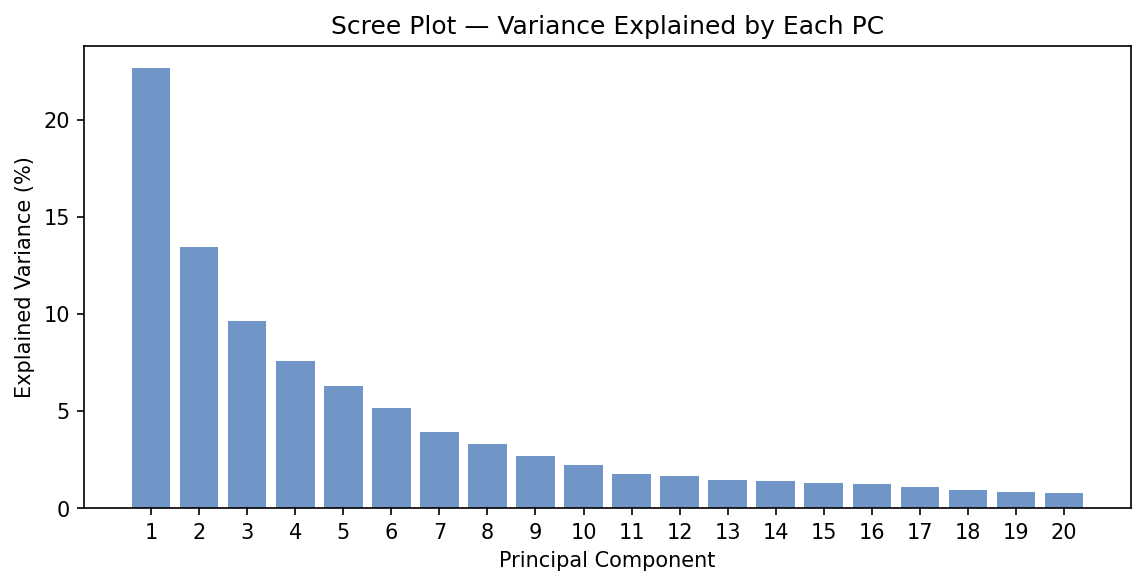
\includegraphics[width=0.82\textwidth]{pca_scree_plot.png}
    \caption{Scree plot: proportion of total variance explained by each
    principal component. The contribution decreases steeply after the
    first few components.}
    \label{fig:pca_scree}
\end{figure}

\begin{figure}[htbp]
    \centering
    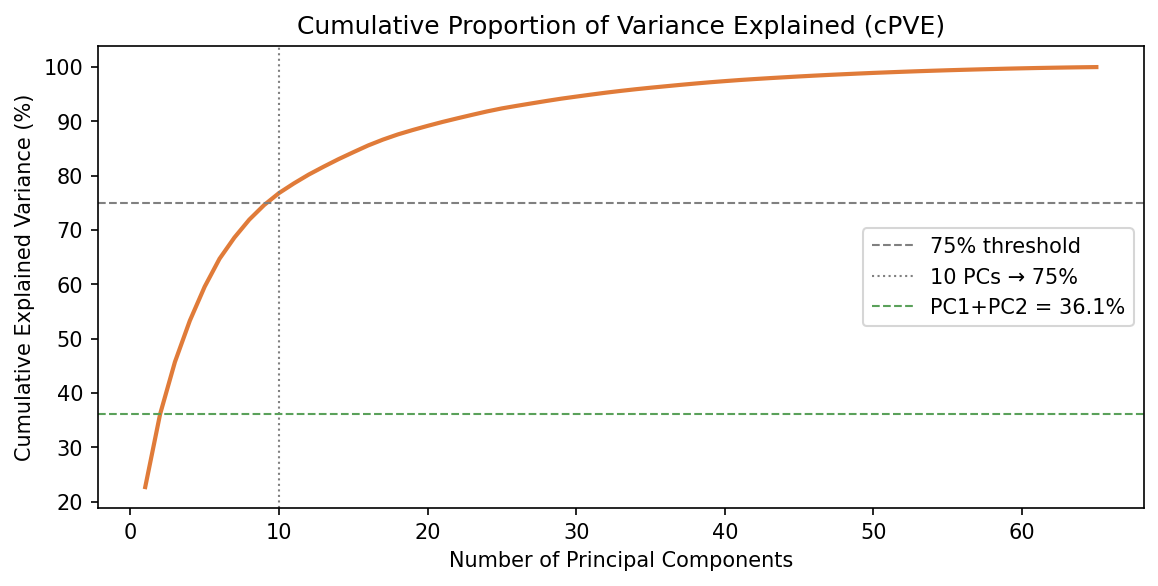
\includegraphics[width=0.82\textwidth]{pca_cumulative_variance.png}
    \caption{Cumulative proportion of variance explained (cPVE).
    The dashed horizontal line marks the 75\% threshold, reached at
    approximately 10 components.}
    \label{fig:pca_cumvar}
\end{figure}

\paragraph{Projection onto the first two components.}
Figure~\ref{fig:pca_biplot} shows the 428 training observations projected
onto the plane defined by PC1 and PC2, coloured by morphosyntactic class.
Following the biplot framework described in \cite{james2013isl},
the loading vectors reveal the semantic interpretation of each axis.
PC1 is dominated by sensorimotor features
(\textsc{Vision}, \textsc{Colour}, \textsc{Shape}, \textsc{Touch},
\textsc{Texture}), tracing a \emph{concreteness} gradient along which
nouns (\emph{Thing}) cluster toward the concrete pole.
PC2 captures auditory and affective features
(\textsc{Fast}, \textsc{Sound}, \textsc{Pain}, \textsc{Attention},
\textsc{Loud}), separating more dynamic or eventive concepts from
static ones.
A broad but imperfect separation between word classes is visible,
suggesting that the feature space encodes class-relevant variation,
though the boundaries are not sharp.

\begin{figure}[htbp]
    \centering
    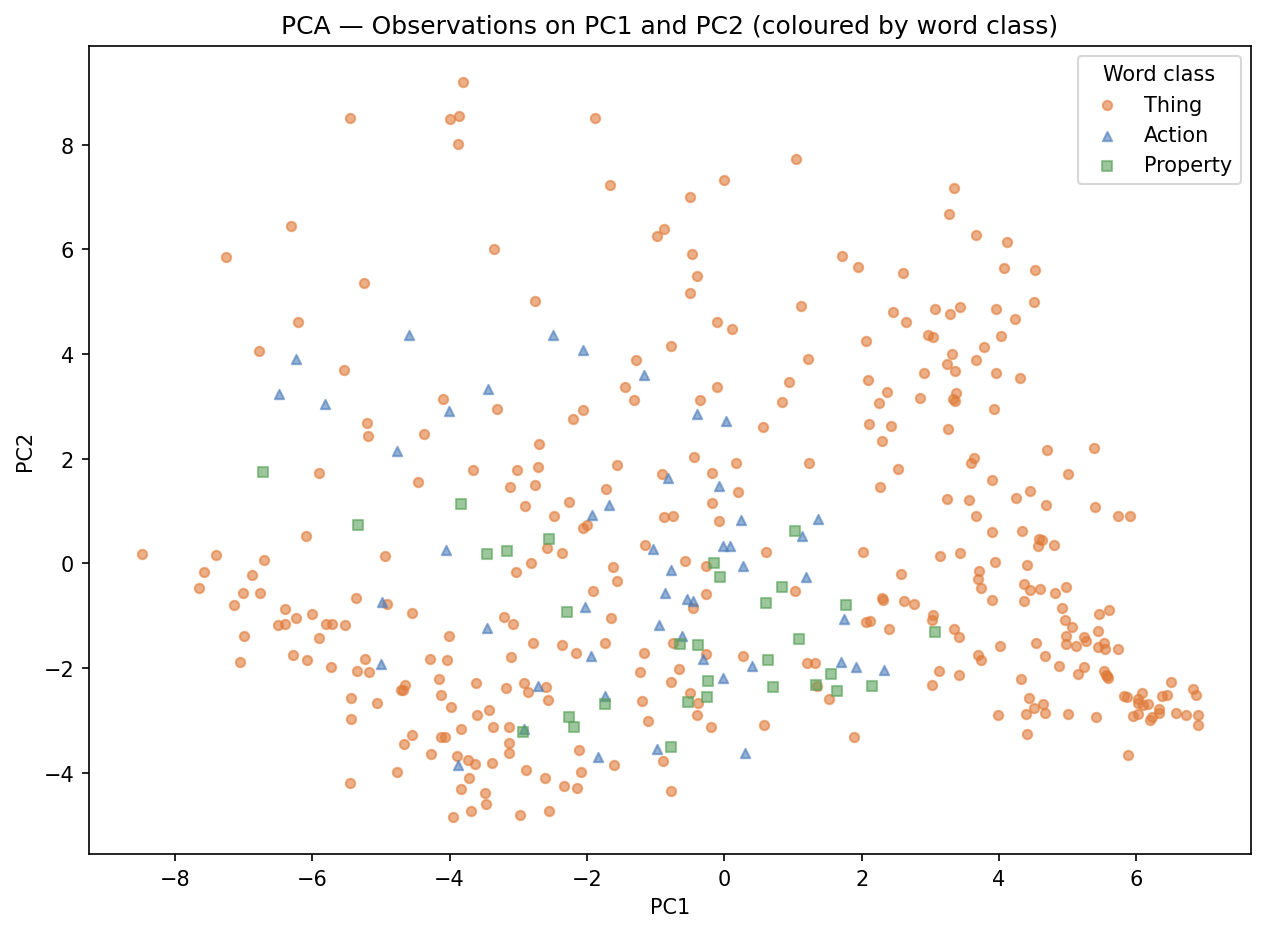
\includegraphics[width=0.85\textwidth]{pca_biplot_pc1_pc2.png}
    \caption{Training observations projected onto PC1 and PC2.
    Colours indicate morphosyntactic class:
    \emph{Thing} (nouns), \emph{Action} (verbs), \emph{Property} (adjectives).
    A concreteness gradient is visible along PC1.}
    \label{fig:pca_biplot}
\end{figure}

% ------------------------------------------------------------------
\subsubsection*{Clustering}

Clustering was performed on the PCA-reduced space retaining the first
10 principal components (those accounting for approximately 75\% of the
variance).
Operating in this reduced space attenuates the effect of noise and
high dimensionality on distance computations\cite{james2013isl},
which notes that many statistical techniques, including clustering,
can benefit from using the first few principal component score vectors
rather than the full feature matrix.

Two methods were applied: $K$-means clustering and Agglomerative
Hierarchical Clustering (AHC) with complete linkage and Euclidean distance,
both introduced in \cite{james2013isl}.

\paragraph{Selecting the number of clusters.}
The optimal $K$ was investigated using two criteria.

\begin{enumerate}
    \item \textbf{Elbow method} ($K$-means): the within-cluster inertia was
    plotted as a function of $K$ (Figure~\ref{fig:kmeans_elbow}).
    As noted in \cite{james2013isl}, minimising the
    within-cluster variation is the objective of $K$-means; the elbow
    in the inertia curve indicates where additional clusters yield
    diminishing returns.
    The Hartigan index, defined as
    $H(K) = \bigl(\mathrm{inertia}(K)/\mathrm{inertia}(K{+}1) - 1\bigr)(n - K - 1)$,
    formalises this criterion; both point to $K = 2$ as the most
    parsimonious solution.

    \item \textbf{Average silhouette score}: the mean silhouette coefficient
    was computed for $K \in \{2, \ldots, 15\}$ for both methods
    (Figures~\ref{fig:kmeans_sil} and~\ref{fig:ahc_sil}).
    The silhouette scores are modest throughout, reflecting the absence
    of strongly separated clusters in this data. The highest values
    are obtained at small $K$, with $K = 2$ yielding approximately
    $0.43$ for $K$-means and $0.16$ for AHC.
\end{enumerate}

\begin{figure}[htbp]
    \centering
    \begin{minipage}[t]{0.48\textwidth}
        \centering
        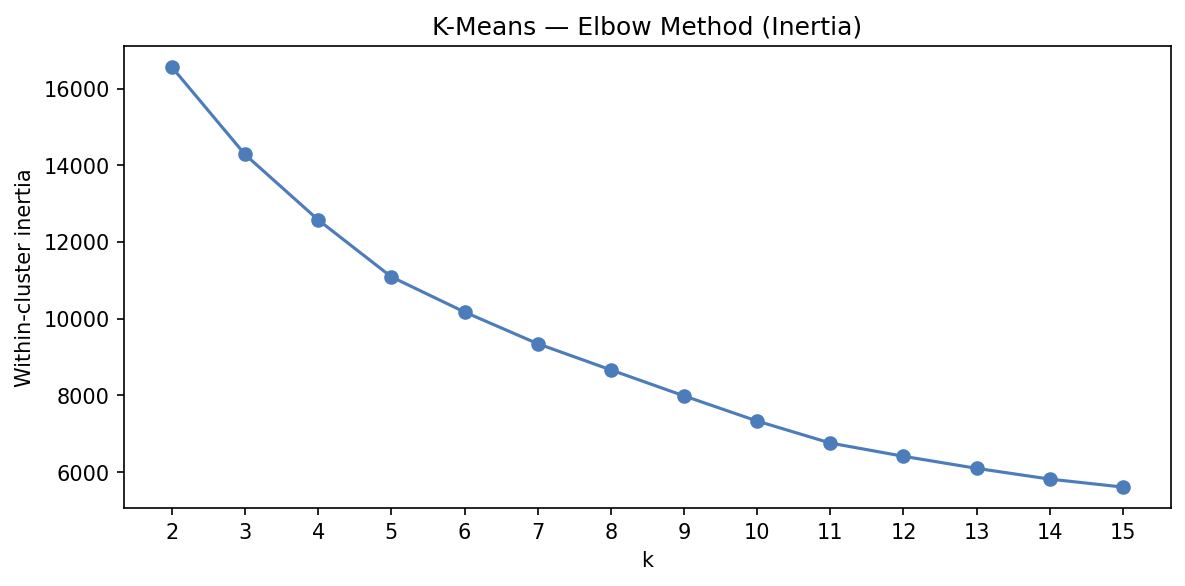
\includegraphics[width=\textwidth]{kmeans_elbow_inertia.png}
        \caption{$K$-means: within-cluster inertia (elbow method).}
        \label{fig:kmeans_elbow}
    \end{minipage}
    \hfill
    \begin{minipage}[t]{0.48\textwidth}
        \centering
        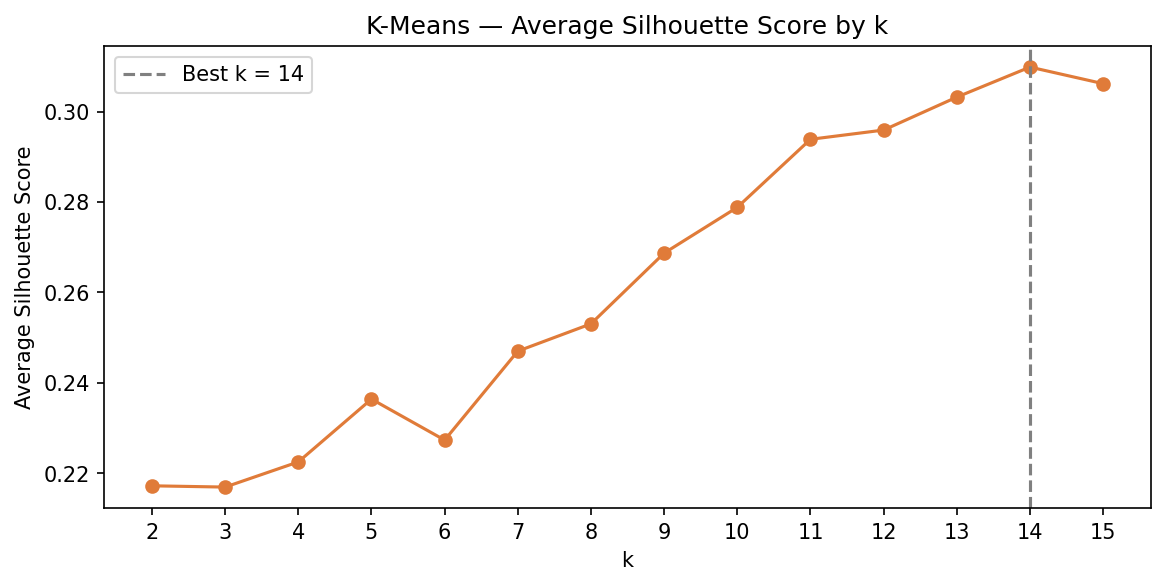
\includegraphics[width=\textwidth]{kmeans_silhouette_by_k.png}
        \caption{$K$-means: average silhouette score by $K$.}
        \label{fig:kmeans_sil}
    \end{minipage}
\end{figure}

\begin{figure}[htbp]
    \centering
    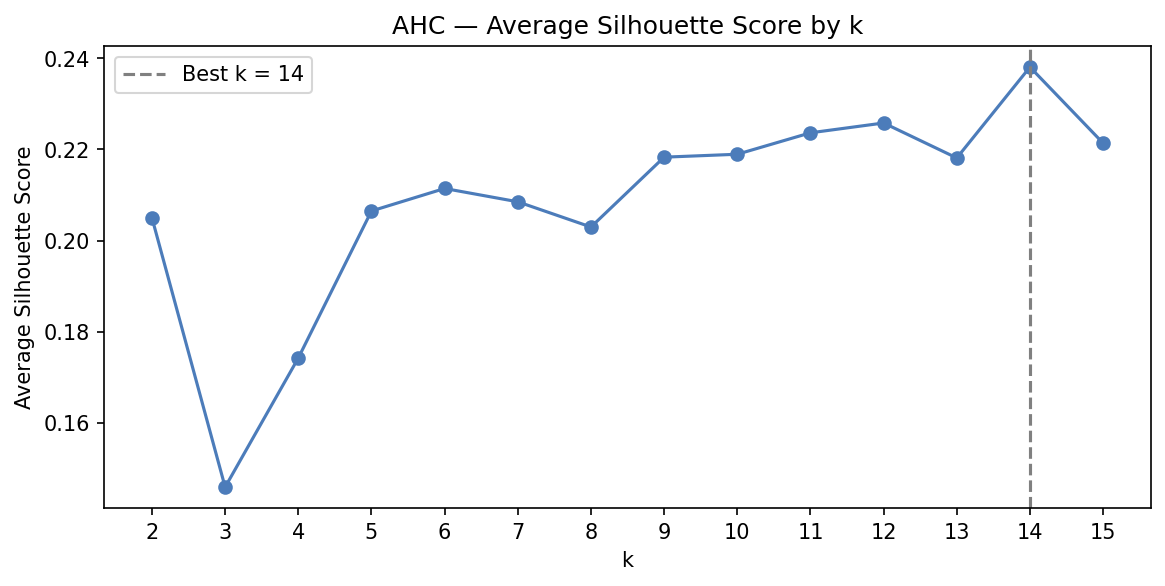
\includegraphics[width=0.65\textwidth]{ahc_silhouette_by_k.png}
    \caption{AHC (complete linkage, Euclidean distance): average
    silhouette score by $K$.}
    \label{fig:ahc_sil}
\end{figure}

Given the flat silhouette profile, two values of $K$ are considered
in the visualisations: $K = 2$ (indicated by both criteria) and
$K = 10$ (a semantically richer partition).
An important caveat noted in \cite{james2013isl} is that
$K$-means finds a \emph{local} rather than global optimum; for this
reason the algorithm was run with 20 random initialisations and the
solution minimising the objective was retained.

\begin{figure}[htbp]
    \centering
    \begin{minipage}[t]{0.48\textwidth}
        \centering
        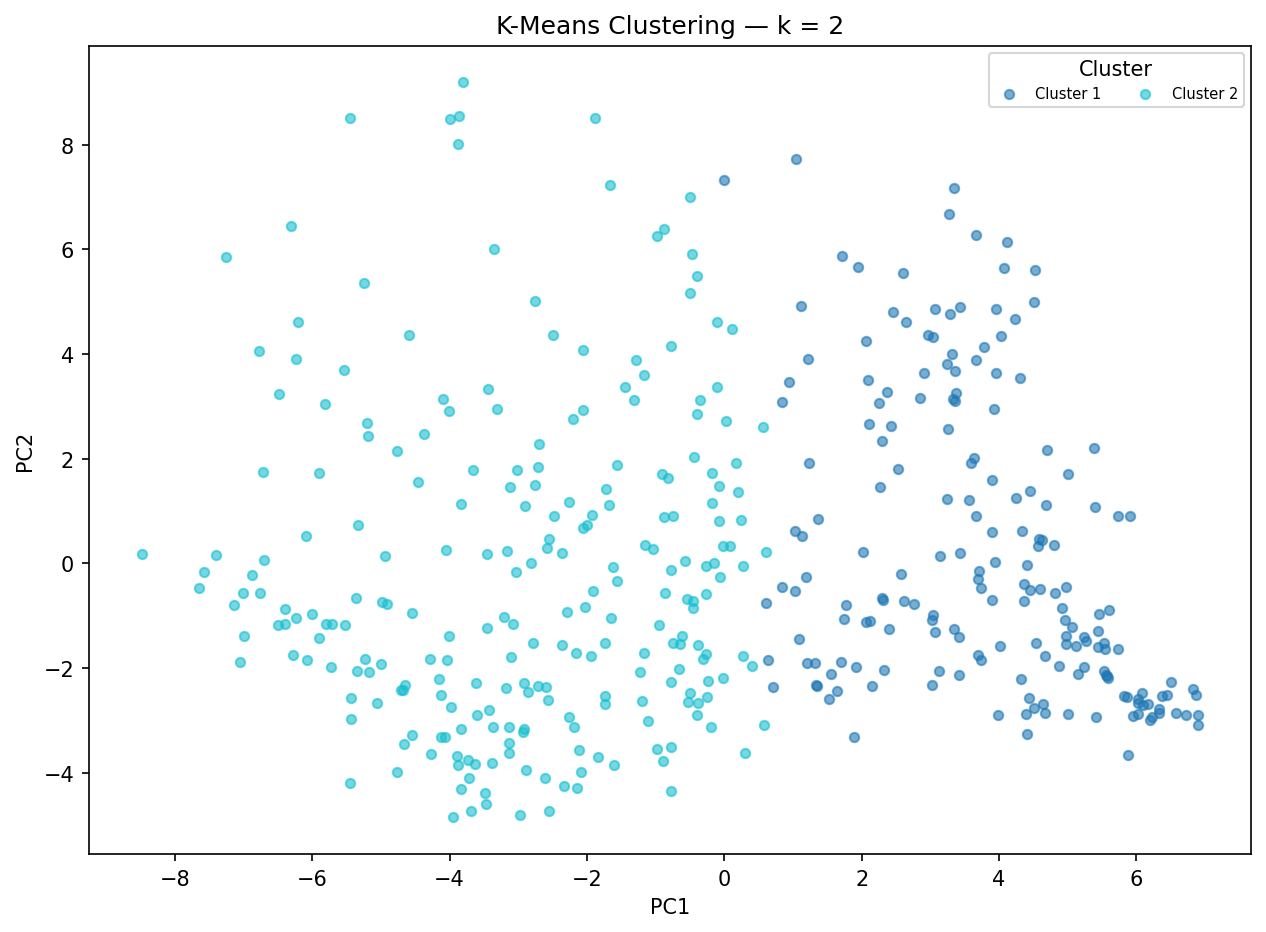
\includegraphics[width=\textwidth]{kmeans_clusters_pc12_k2.png}
        \caption{$K$-means, $K=2$: the partition roughly follows the
        concreteness gradient of PC1.}
        \label{fig:km_k2}
    \end{minipage}
    \hfill
    \begin{minipage}[t]{0.48\textwidth}
        \centering
        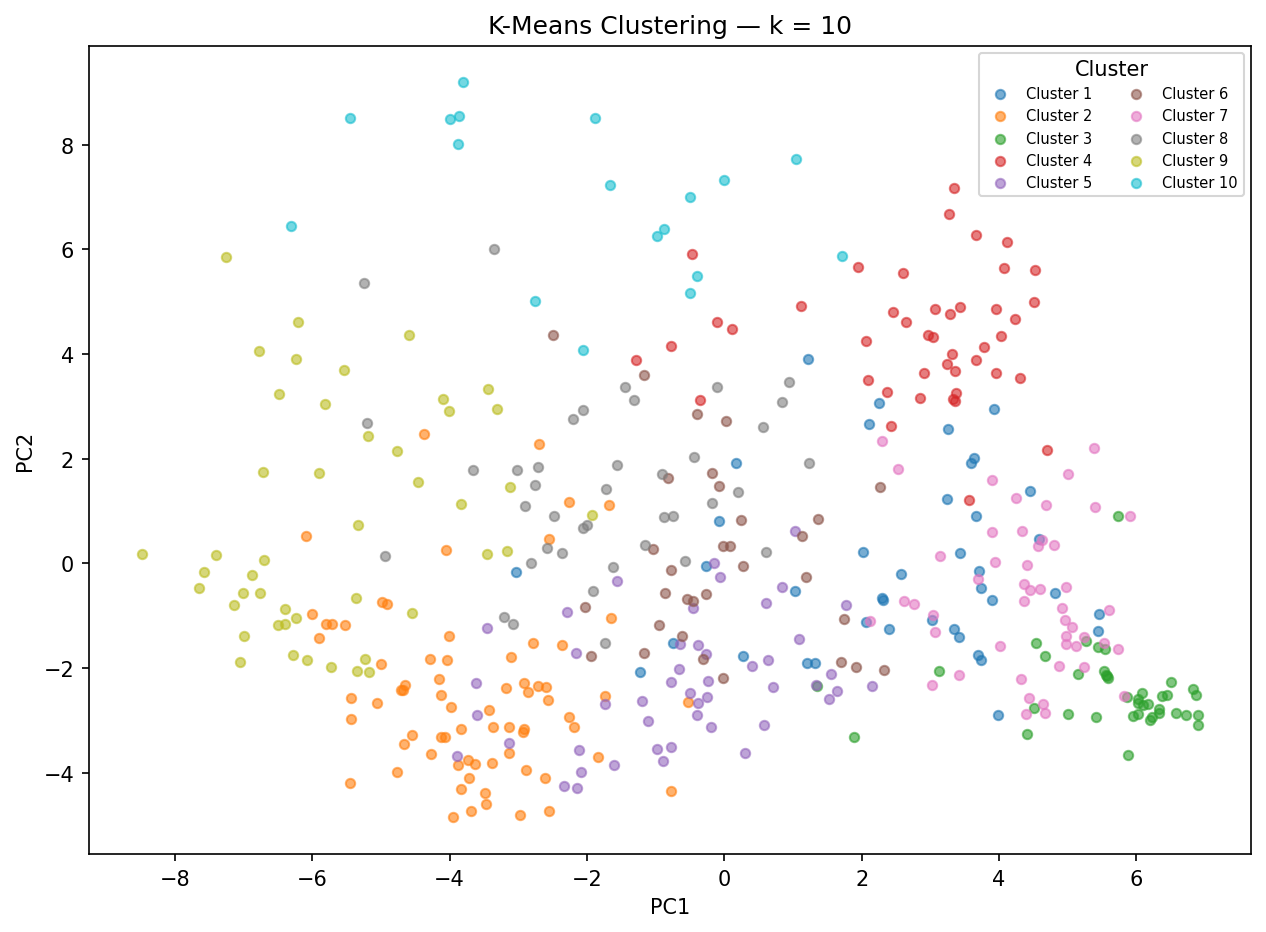
\includegraphics[width=\textwidth]{kmeans_clusters_pc12_k10.png}
        \caption{$K$-means, $K=10$: finer-grained semantic domains
        begin to emerge.}
        \label{fig:km_k10}
    \end{minipage}
\end{figure}

\begin{figure}[htbp]
    \centering
    \begin{minipage}[t]{0.48\textwidth}
        \centering
        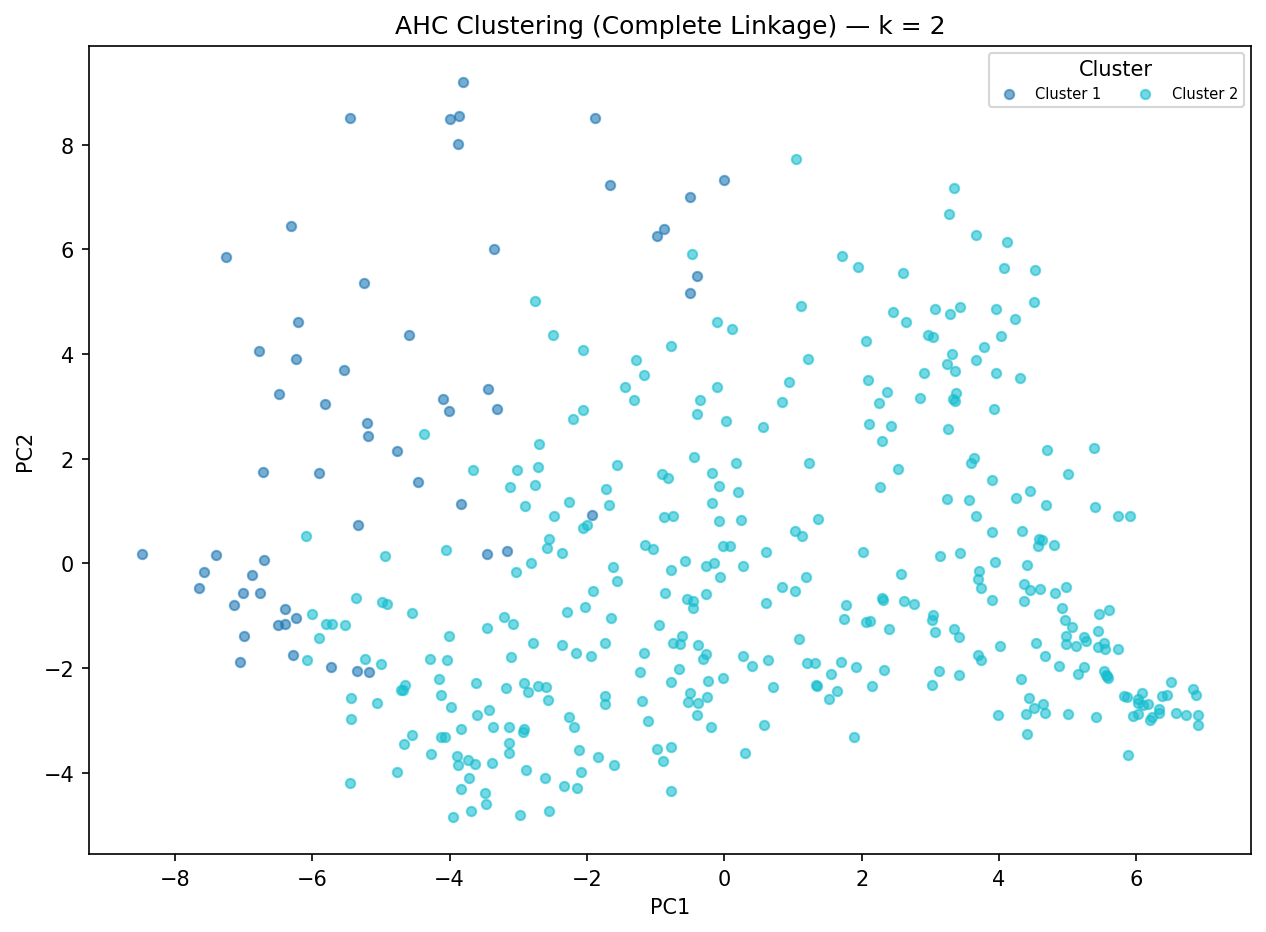
\includegraphics[width=\textwidth]{ahc_clusters_pc12_k2.png}
        \caption{AHC, $K=2$.}
        \label{fig:ahc_k2}
    \end{minipage}
    \hfill
    \begin{minipage}[t]{0.48\textwidth}
        \centering
        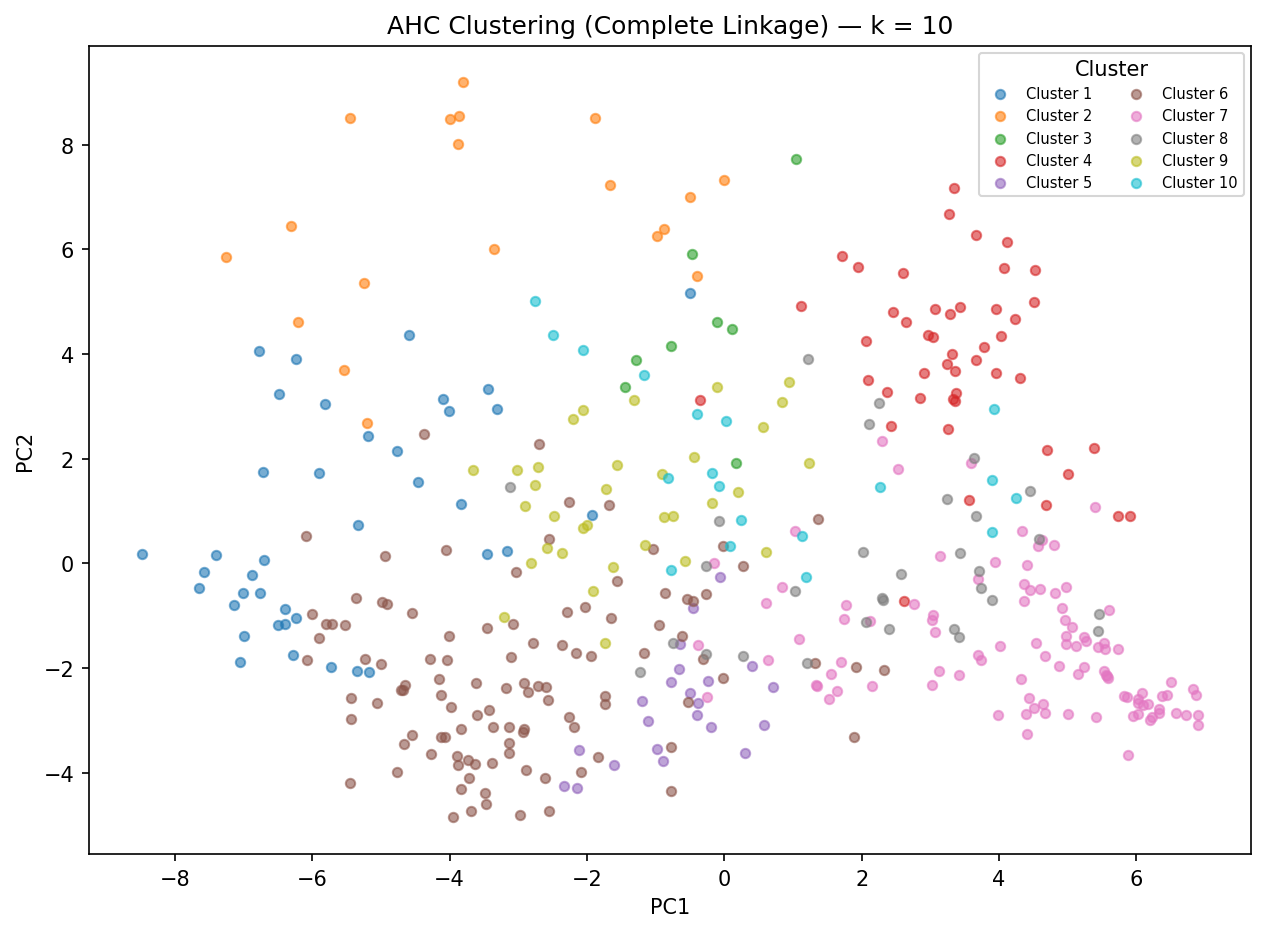
\includegraphics[width=\textwidth]{ahc_clusters_pc12_k10.png}
        \caption{AHC, $K=10$: qualitatively more coherent semantic
        groupings than $K$-means (e.g.\ animals, food, negative affect).}
        \label{fig:ahc_k10}
    \end{minipage}
\end{figure}

% ------------------------------------------------------------------
\subsubsection*{Comparison with known labels}

To assess the degree of correspondence between the data-driven cluster
structure and the three morphosyntactic classes
(\emph{Thing}, \emph{Action}, \emph{Property}), the cluster assignments
at $K = 3$ were compared with the ground-truth labels using two
external validity indices: the Adjusted Rand Index (ARI) and the
Normalised Mutual Information (NMI).
These metrics are not introduced in \cite{james2013isl} but are
standard in the clustering evaluation literature; ARI equals 1 for a
perfect match and is 0 in expectation for a random partition.

Table~\ref{tab:cluster_comparison} reports ARI and NMI for both methods
at $K = 3$.

\begin{table}[htbp]
    \centering
    \caption{External validity of cluster assignments at $K=3$ compared
    with the three morphosyntactic labels. Values to be filled after
    running \texttt{phase2\_unsupervised.py} and reading from
    \texttt{outputs/II/phase2\_unsupervised/phase2\_summary.json}.}
    \label{tab:cluster_comparison}
    \begin{tabular}{lcc}
        \toprule
        \textbf{Method} & \textbf{ARI} & \textbf{NMI} \\
        \midrule
        $K$-means ($K=3$) & \texttt{---} & \texttt{---} \\
        AHC ($K=3$)       & \texttt{---} & \texttt{---} \\
        \bottomrule
    \end{tabular}
\end{table}

\begin{figure}[htbp]
    \centering
    \begin{minipage}[t]{0.48\textwidth}
        \centering
        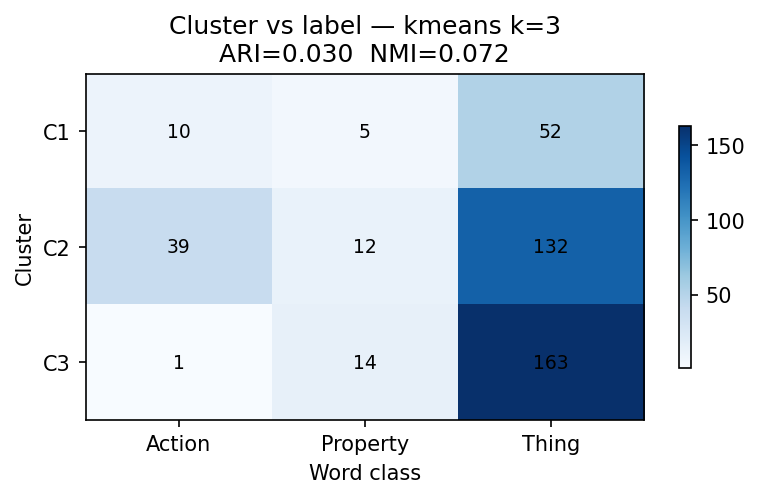
\includegraphics[width=\textwidth]{cluster_vs_label_kmeans_k3.png}
        \caption{Cluster--label correspondence heatmap, $K$-means $K=3$.}
    \end{minipage}
    \hfill
    \begin{minipage}[t]{0.48\textwidth}
        \centering
        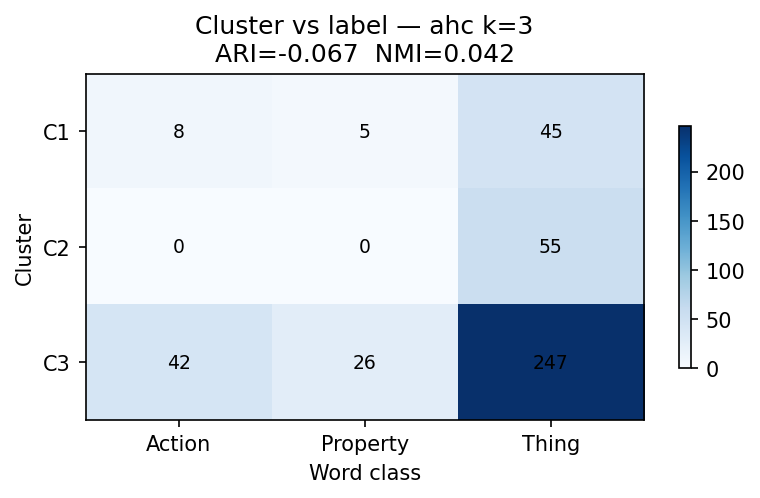
\includegraphics[width=\textwidth]{cluster_vs_label_ahc_k3.png}
        \caption{Cluster--label correspondence heatmap, AHC $K=3$.}
    \end{minipage}
\end{figure}

% ------------------------------------------------------------------
\subsubsection*{Interpretation}

The unsupervised analysis yields three main findings.

First, the data-driven cluster structure does \emph{not} align strongly
with the morphosyntactic partition. This is consistent with the intrinsic
difficulty of the task: the three word classes are not cleanly separable
in the semantic feature space, and the dataset is strongly imbalanced
(nouns account for approximately 81\% of the training set).

Second, at $K = 2$, both methods identify a broad
\textbf{concrete vs.\ abstract} dimension that cuts across
morphosyntactic boundaries. The concrete cluster is dominated by nouns
referring to physical entities (e.g.\ \emph{elephant}, \emph{bread}),
but also contains action verbs denoting physical events.
The abstract cluster groups most verbs and adjectives together with
nouns referring to mental or social concepts.
This concrete--abstract axis corresponds to the first principal component
and is the most prominent structure in the feature space.

Third, at $K = 10$, AHC with complete linkage recovers several
semantically coherent groups — including clusters of animal names,
food items, sounds, and negatively valenced concepts — that correspond
to fine-grained \emph{semantic categories} rather than to the
grammatical classes of interest.
This confirms that the 65-dimensional feature space encodes rich
semantic similarity information at a level of granularity finer than
the noun/verb/adjective distinction, and motivates the use of a
supervised approach for the classification task.

These results serve a diagnostic function in the overall pipeline:
they confirm the semantic informativeness of the feature space while
showing that the class labels are not trivially recoverable from
unsupervised exploration alone.


\subsection{III. Supervised classification on the original feature space}

In this phase, we formulate a multiclass supervised learning problem aimed at predicting the lexical-semantic labels (\emph{Thing}, \emph{Action}, \emph{Property}) from the original semantic feature space. The objective is to quantify how much of the categorical structure of lexical meaning is captured by the experiential attributes and to understand the role of redundancy, multicollinearity, and model complexity in this setting.

\paragraph{Baseline model}

We begin with a multinomial logistic regression model, which provides a natural baseline within the generalized linear model framework. This model assumes a linear relationship between the predictors and the log-odds of class membership and serves as a reference point for all subsequent analyses.

The baseline achieves strong performance, as reported in Table~\ref{tab:phase3_baseline}.

\begin{table}[H]
\centering
\begin{tabular}{lcc}
\hline
Model & Accuracy & Macro F1 \\
\hline
Multinomial Logistic baseline & 0.9533 & 0.8904 \\
\hline
\end{tabular}
\caption{Baseline multinomial logistic regression performance on the original labels.}
\label{tab:phase3_baseline}
\end{table}

The high accuracy indicates that the semantic feature space is highly informative. However, the lower macro F1 (0.8904) compared to accuracy suggests an imbalance in class-wise performance, meaning that some classes are easier to predict than others.

This behavior is confirmed by the confusion matrix in Figure~\ref{fig:phase3_baseline_cm}.

\begin{figure}[H]
\centering
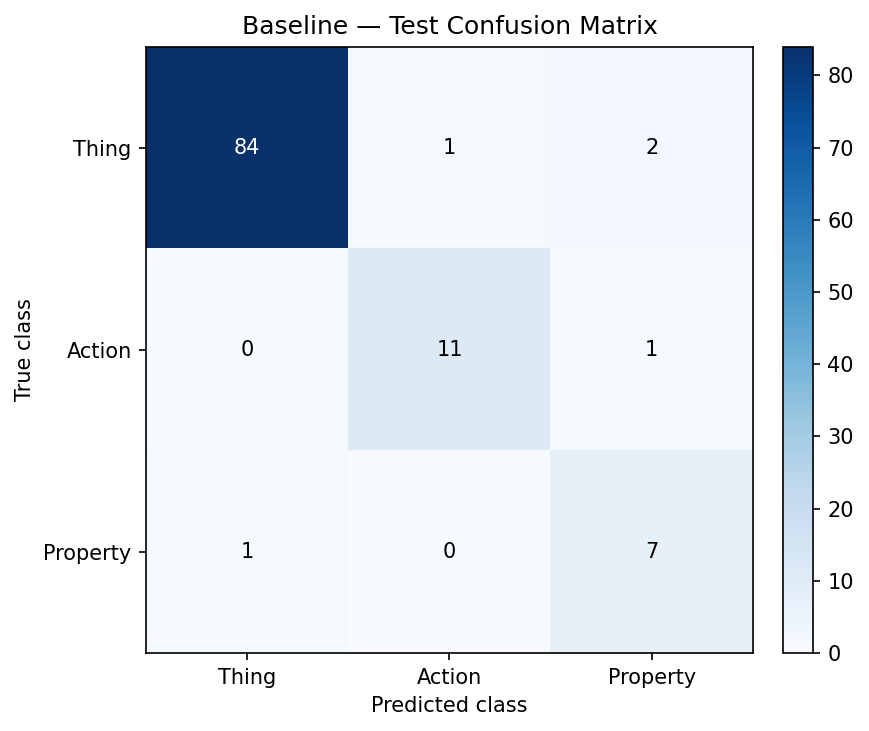
\includegraphics[width=0.6\textwidth]{baseline_confusion_matrix_test.png}
\caption{Confusion matrix of the baseline multinomial logistic regression.}
\label{fig:phase3_baseline_cm}
\end{figure}

From the confusion matrix, it is evident that misclassifications are not uniformly distributed across classes, indicating overlapping regions in the feature space.

\paragraph{Multicollinearity and feature structure}

Before applying more advanced models, we analyze the structure of the feature space. The correlation heatmap in Figure~\ref{fig:phase3_corr_heatmap} shows the presence of strongly correlated blocks of variables.

\begin{figure}[H]
\centering
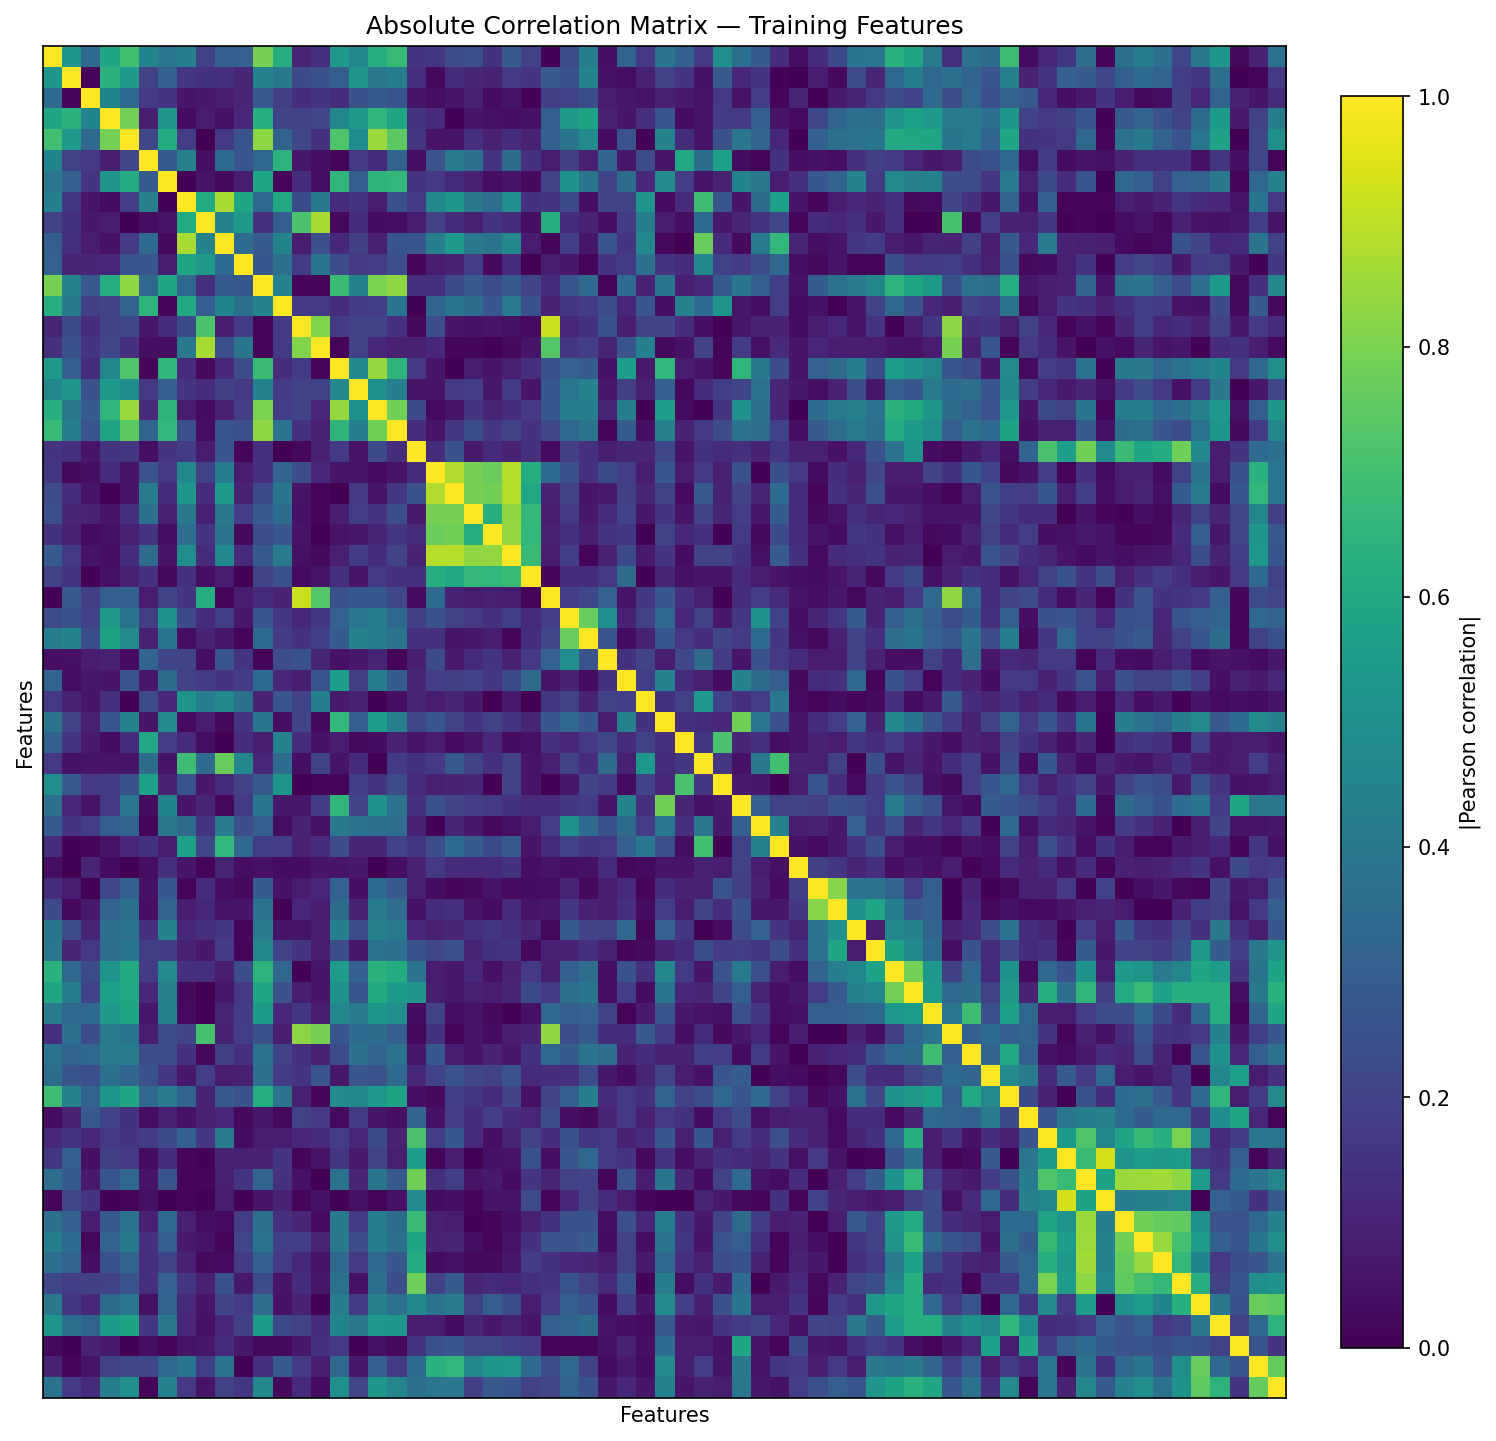
\includegraphics[width=0.8\textwidth]{correlation_heatmap_train.png}
\caption{Correlation heatmap of semantic features.}
\label{fig:phase3_corr_heatmap}
\end{figure}

This structure is further confirmed by the hierarchical clustering of features (Figure~\ref{fig:phase3_feature_dendrogram}), which groups variables into coherent clusters.

\begin{figure}[H]
\centering
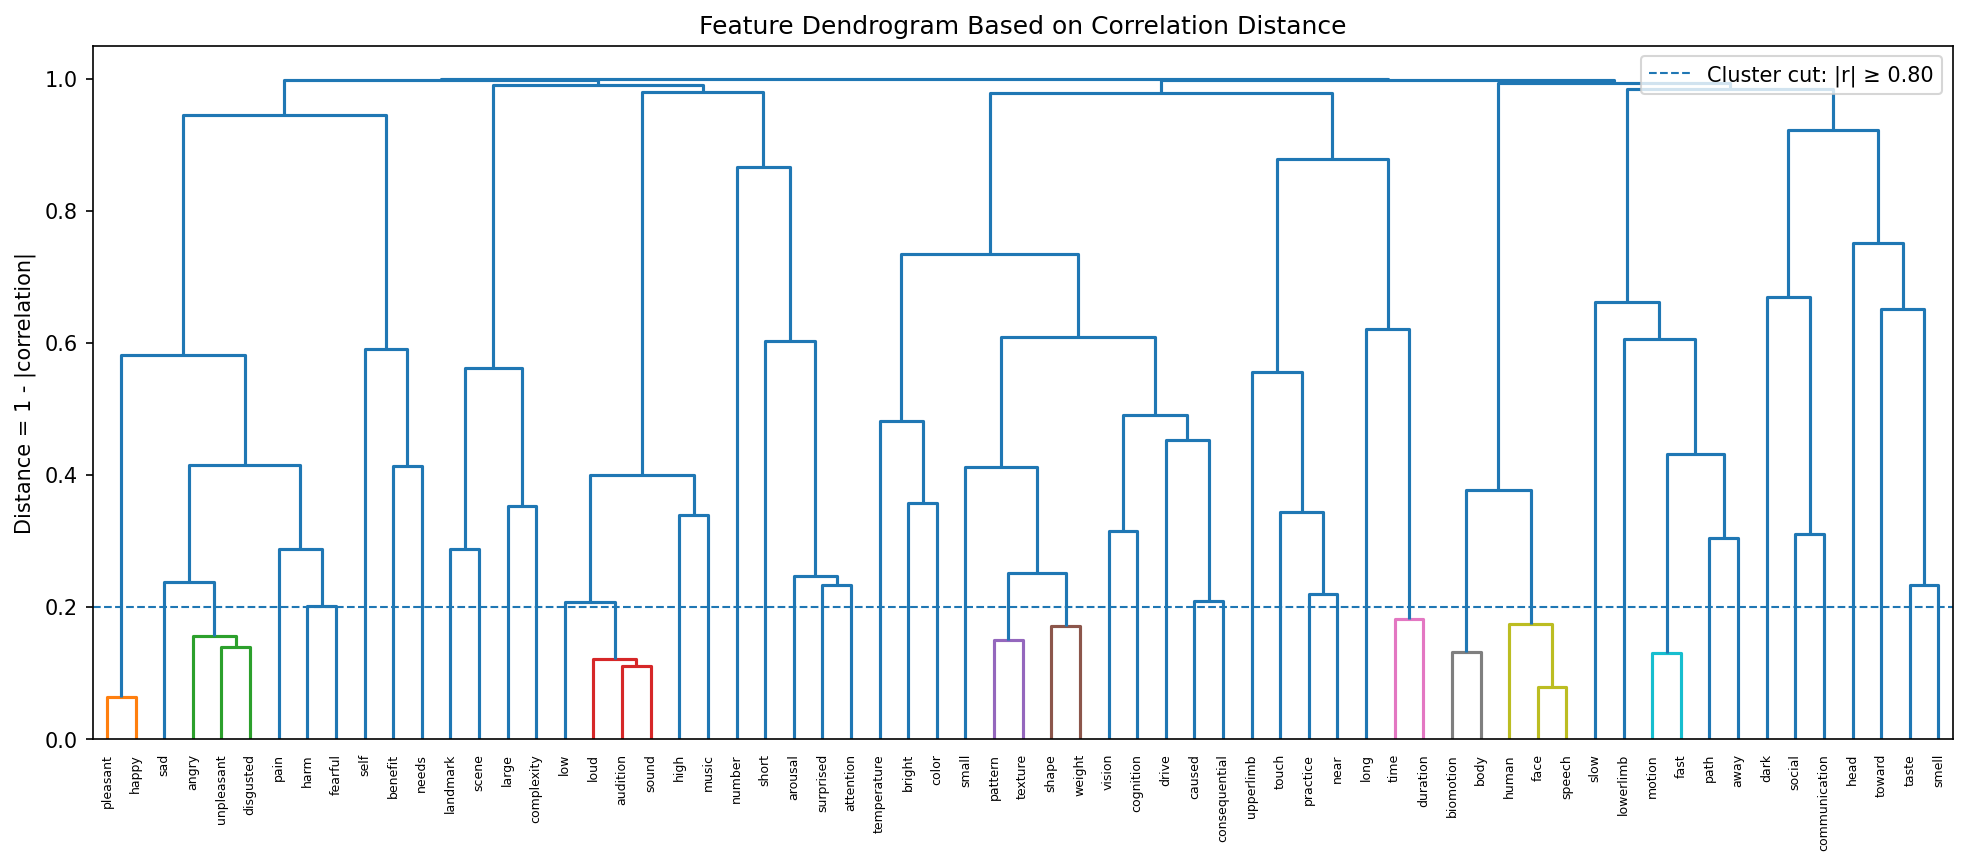
\includegraphics[width=0.8\textwidth]{feature_dendrogram.png}
\caption{Hierarchical clustering dendrogram of features.}
\label{fig:phase3_feature_dendrogram}
\end{figure}

Numerically, this is reflected in the high number of strongly correlated pairs (22 pairs with $|r|\geq 0.8$) and in the presence of many variables with high VIF values (51 features with VIF $\geq 5$). These values confirm that the feature space is highly redundant and that naive models may suffer from instability.

\paragraph{Regularized models}

To address multicollinearity and improve generalization, we apply LASSO and Elastic Net regularized multinomial logistic regression models.

\begin{table}[H]
\centering
\begin{tabular}{lcc}
\hline
Model & Accuracy & Macro F1 \\
\hline
LASSO Logistic & 0.9680 & 0.9150 \\
Elastic Net Logistic & 0.9705 & 0.9200 \\
\hline
\end{tabular}
\caption{Performance of regularized multinomial models.}
\label{tab:phase3_regularized}
\end{table}

Both models improve over the baseline, with Elastic Net achieving the best balance between accuracy and macro F1. The improvement in macro F1 (from 0.8904 to 0.9200) is particularly important, as it indicates a more balanced classification across all classes.

\paragraph{Sparsity and feature selection}

Regularization also induces sparsity, reducing the number of active predictors. The most relevant features selected by LASSO are shown in Figure~\ref{fig:phase3_lasso_coeff}.

\begin{figure}[H]
\centering
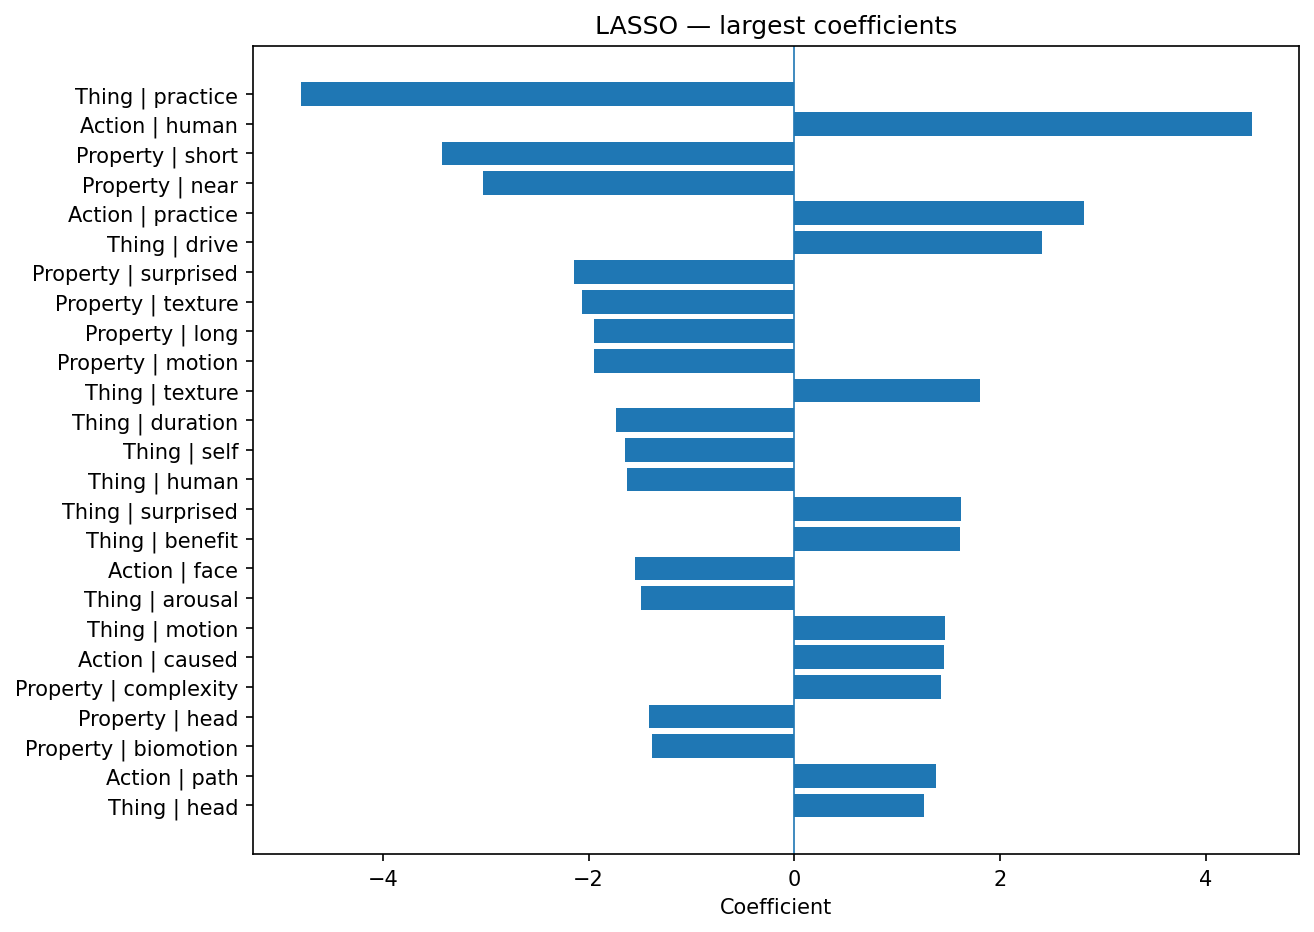
\includegraphics[width=0.75\textwidth]{lasso_top_coefficients.png}
\caption{Top LASSO coefficients.}
\label{fig:phase3_lasso_coeff}
\end{figure}

Elastic Net, shown in Figure~\ref{fig:phase3_enet_coeff}, distributes weights more smoothly across correlated variables.

\begin{figure}[H]
\centering
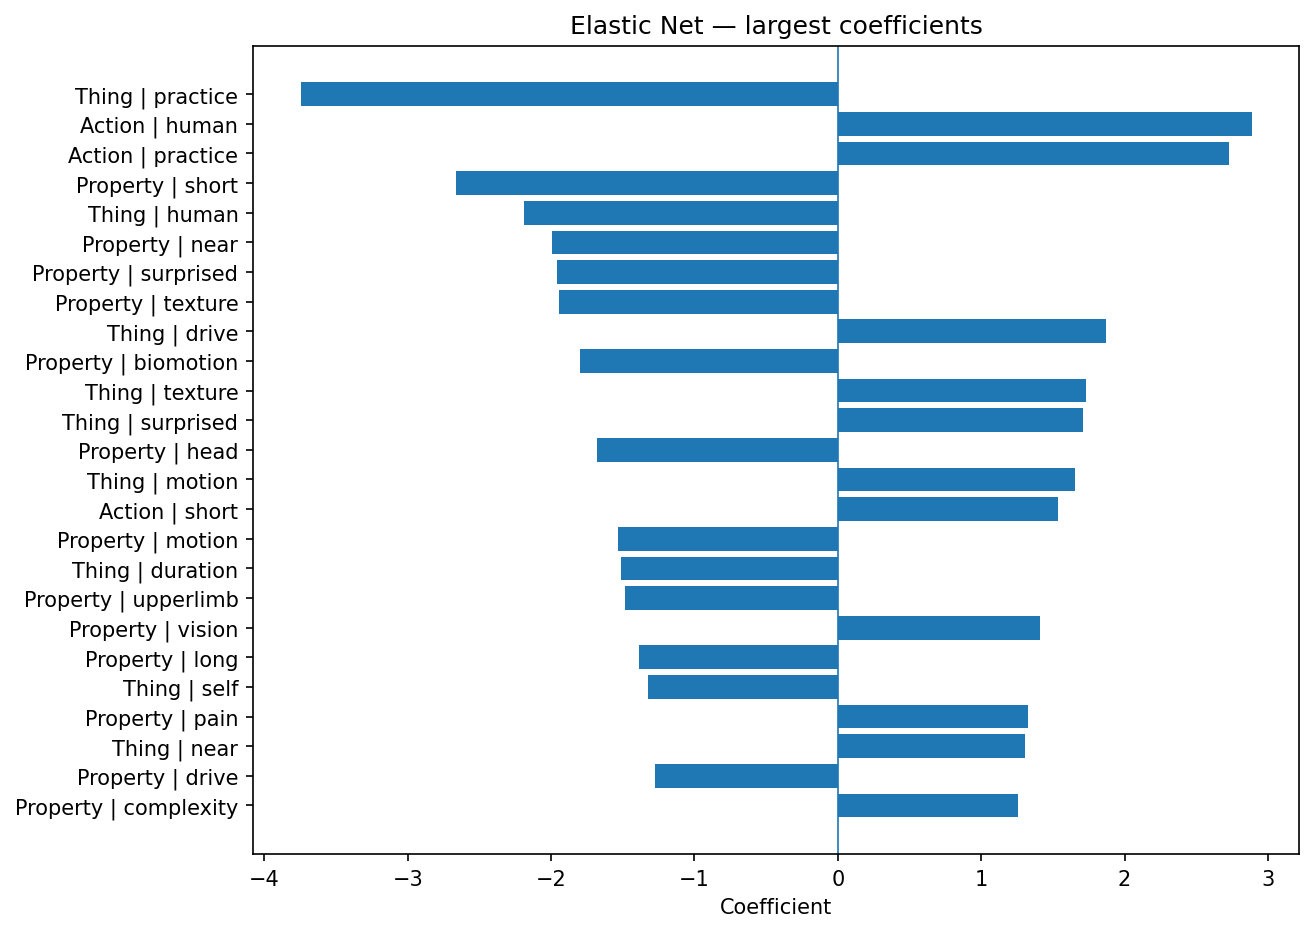
\includegraphics[width=0.75\textwidth]{elastic_net_top_coefficients.png}
\caption{Top Elastic Net coefficients.}
\label{fig:phase3_enet_coeff}
\end{figure}

The sparsity overview in Figure~\ref{fig:phase3_sparsity} shows how many coefficients are effectively used by the models.

\begin{figure}[H]
\centering
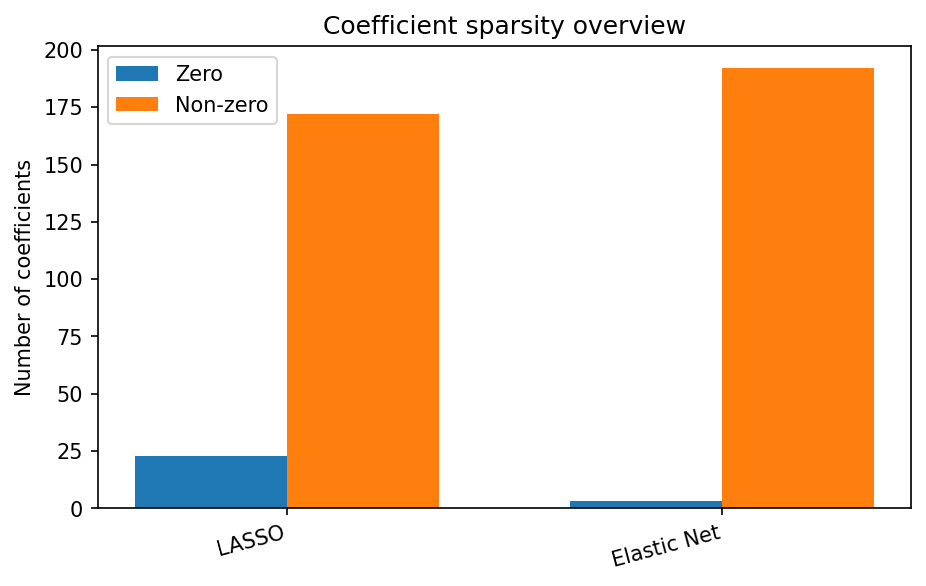
\includegraphics[width=0.7\textwidth]{sparsity_overview.png}
\caption{Sparsity patterns across models.}
\label{fig:phase3_sparsity}
\end{figure}

These results indicate that only a subset of the semantic features is necessary to achieve high predictive performance, confirming the presence of redundancy in the original representation.

\paragraph{Final post-selection model}

After feature selection, we train a final multinomial logistic model on the selected subset.

\begin{table}[H]
\centering
\begin{tabular}{lcc}
\hline
Model & Accuracy & Macro F1 \\
\hline
Post-selection Logistic & 0.9720 & 0.9229 \\
\hline
\end{tabular}
\caption{Final post-selection model.}
\label{tab:phase3_final}
\end{table}

The improvement from 0.9533 to 0.9720 in accuracy and from 0.8904 to 0.9229 in macro F1 demonstrates that removing redundant features improves generalization.

\begin{figure}[H]
\centering
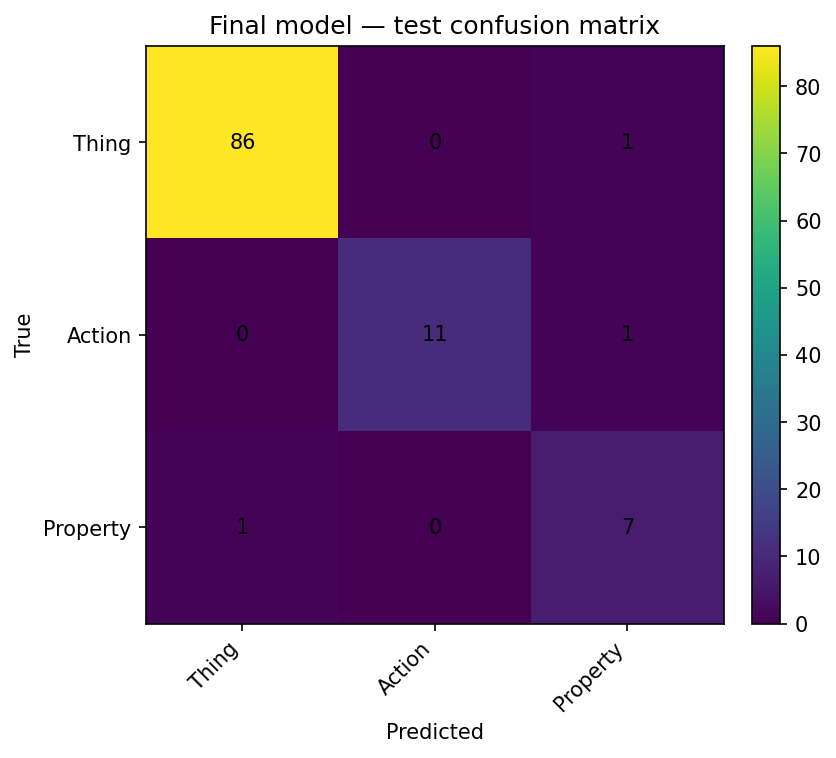
\includegraphics[width=0.6\textwidth]{final_model_confusion_matrix_test.png}
\caption{Confusion matrix of the final model.}
\label{fig:phase3_final_cm}
\end{figure}

\paragraph{Discussion}

Overall, the results show that:
\begin{itemize}
\item the semantic feature space is highly informative;
\item multicollinearity is substantial and must be controlled;
\item regularization improves both stability and performance;
\item a reduced subset of features is sufficient for accurate classification.
\end{itemize}

\vspace{0.5cm}

\subsection{IV. High-dimensional expansion and feature screening}

To further explore the structure of the data, we consider a high-dimensional extension of the feature space. The goal is to increase model expressiveness while controlling for noise and redundancy through feature screening.

\paragraph{Feature screening}

We rank features using ANOVA F-score and mutual information, selecting the most informative subset.

\begin{figure}[H]
\centering
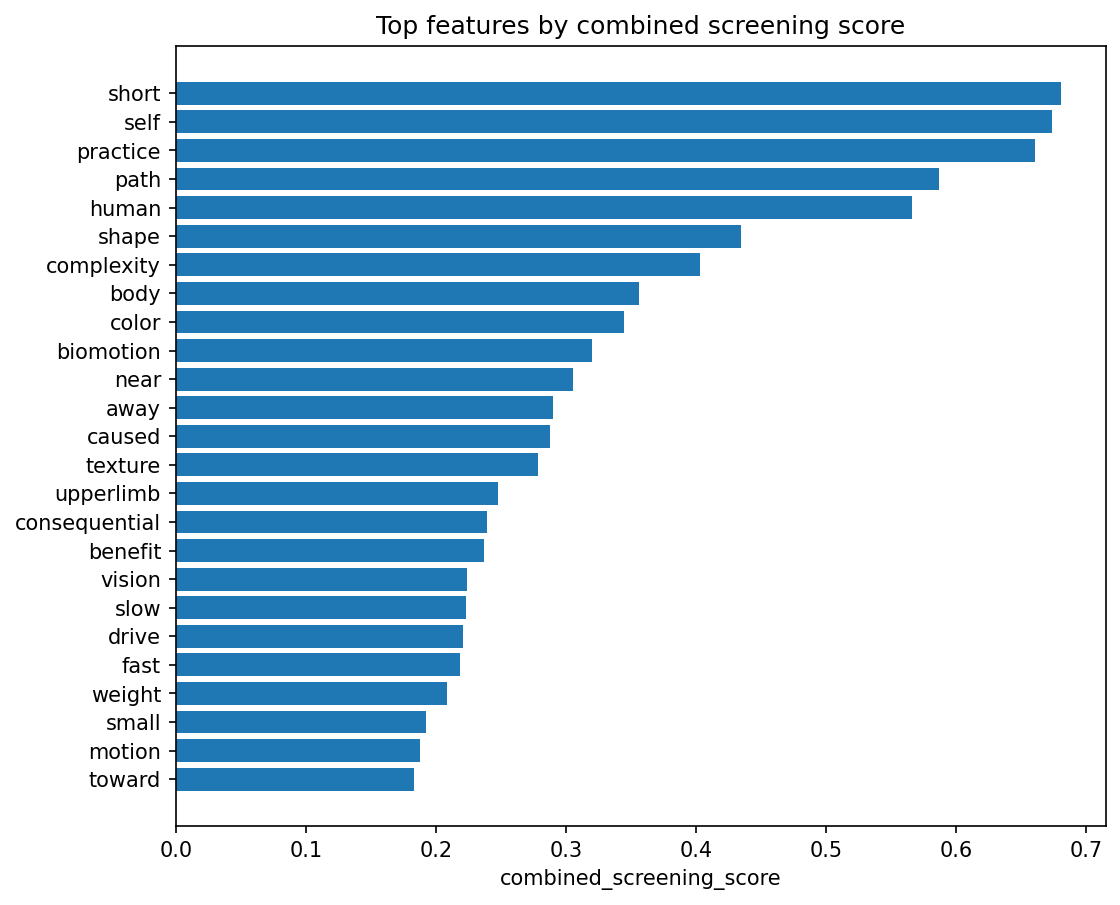
\includegraphics[width=0.7\textwidth]{combined_screening_top_features.png}
\caption{Top features ranked by the combined screening score.}
\label{fig:phase4_combined}
\end{figure}

The ranking shows a steep decay, indicating that a limited number of features carries most of the predictive signal.

\paragraph{Impact}

Screening reduces dimensionality and stabilizes subsequent models, acting as a bridge between raw feature expansion and regularized learning.

\vspace{0.5cm}

\subsection{V. Alternative classifiers}

Finally, we evaluate whether non-linear models can better capture the structure of the data.

\begin{table}[H]
\centering
\begin{tabular}{lcc}
\hline
Model & Accuracy & Macro F1 \\
\hline
Post-selection Logistic & 0.9720 & 0.9229 \\
Random Forest & 0.9813 & 0.9486 \\
\hline
\end{tabular}
\caption{Comparison between linear and non-linear models.}
\label{tab:phase5_models}
\end{table}

\begin{figure}[H]
\centering
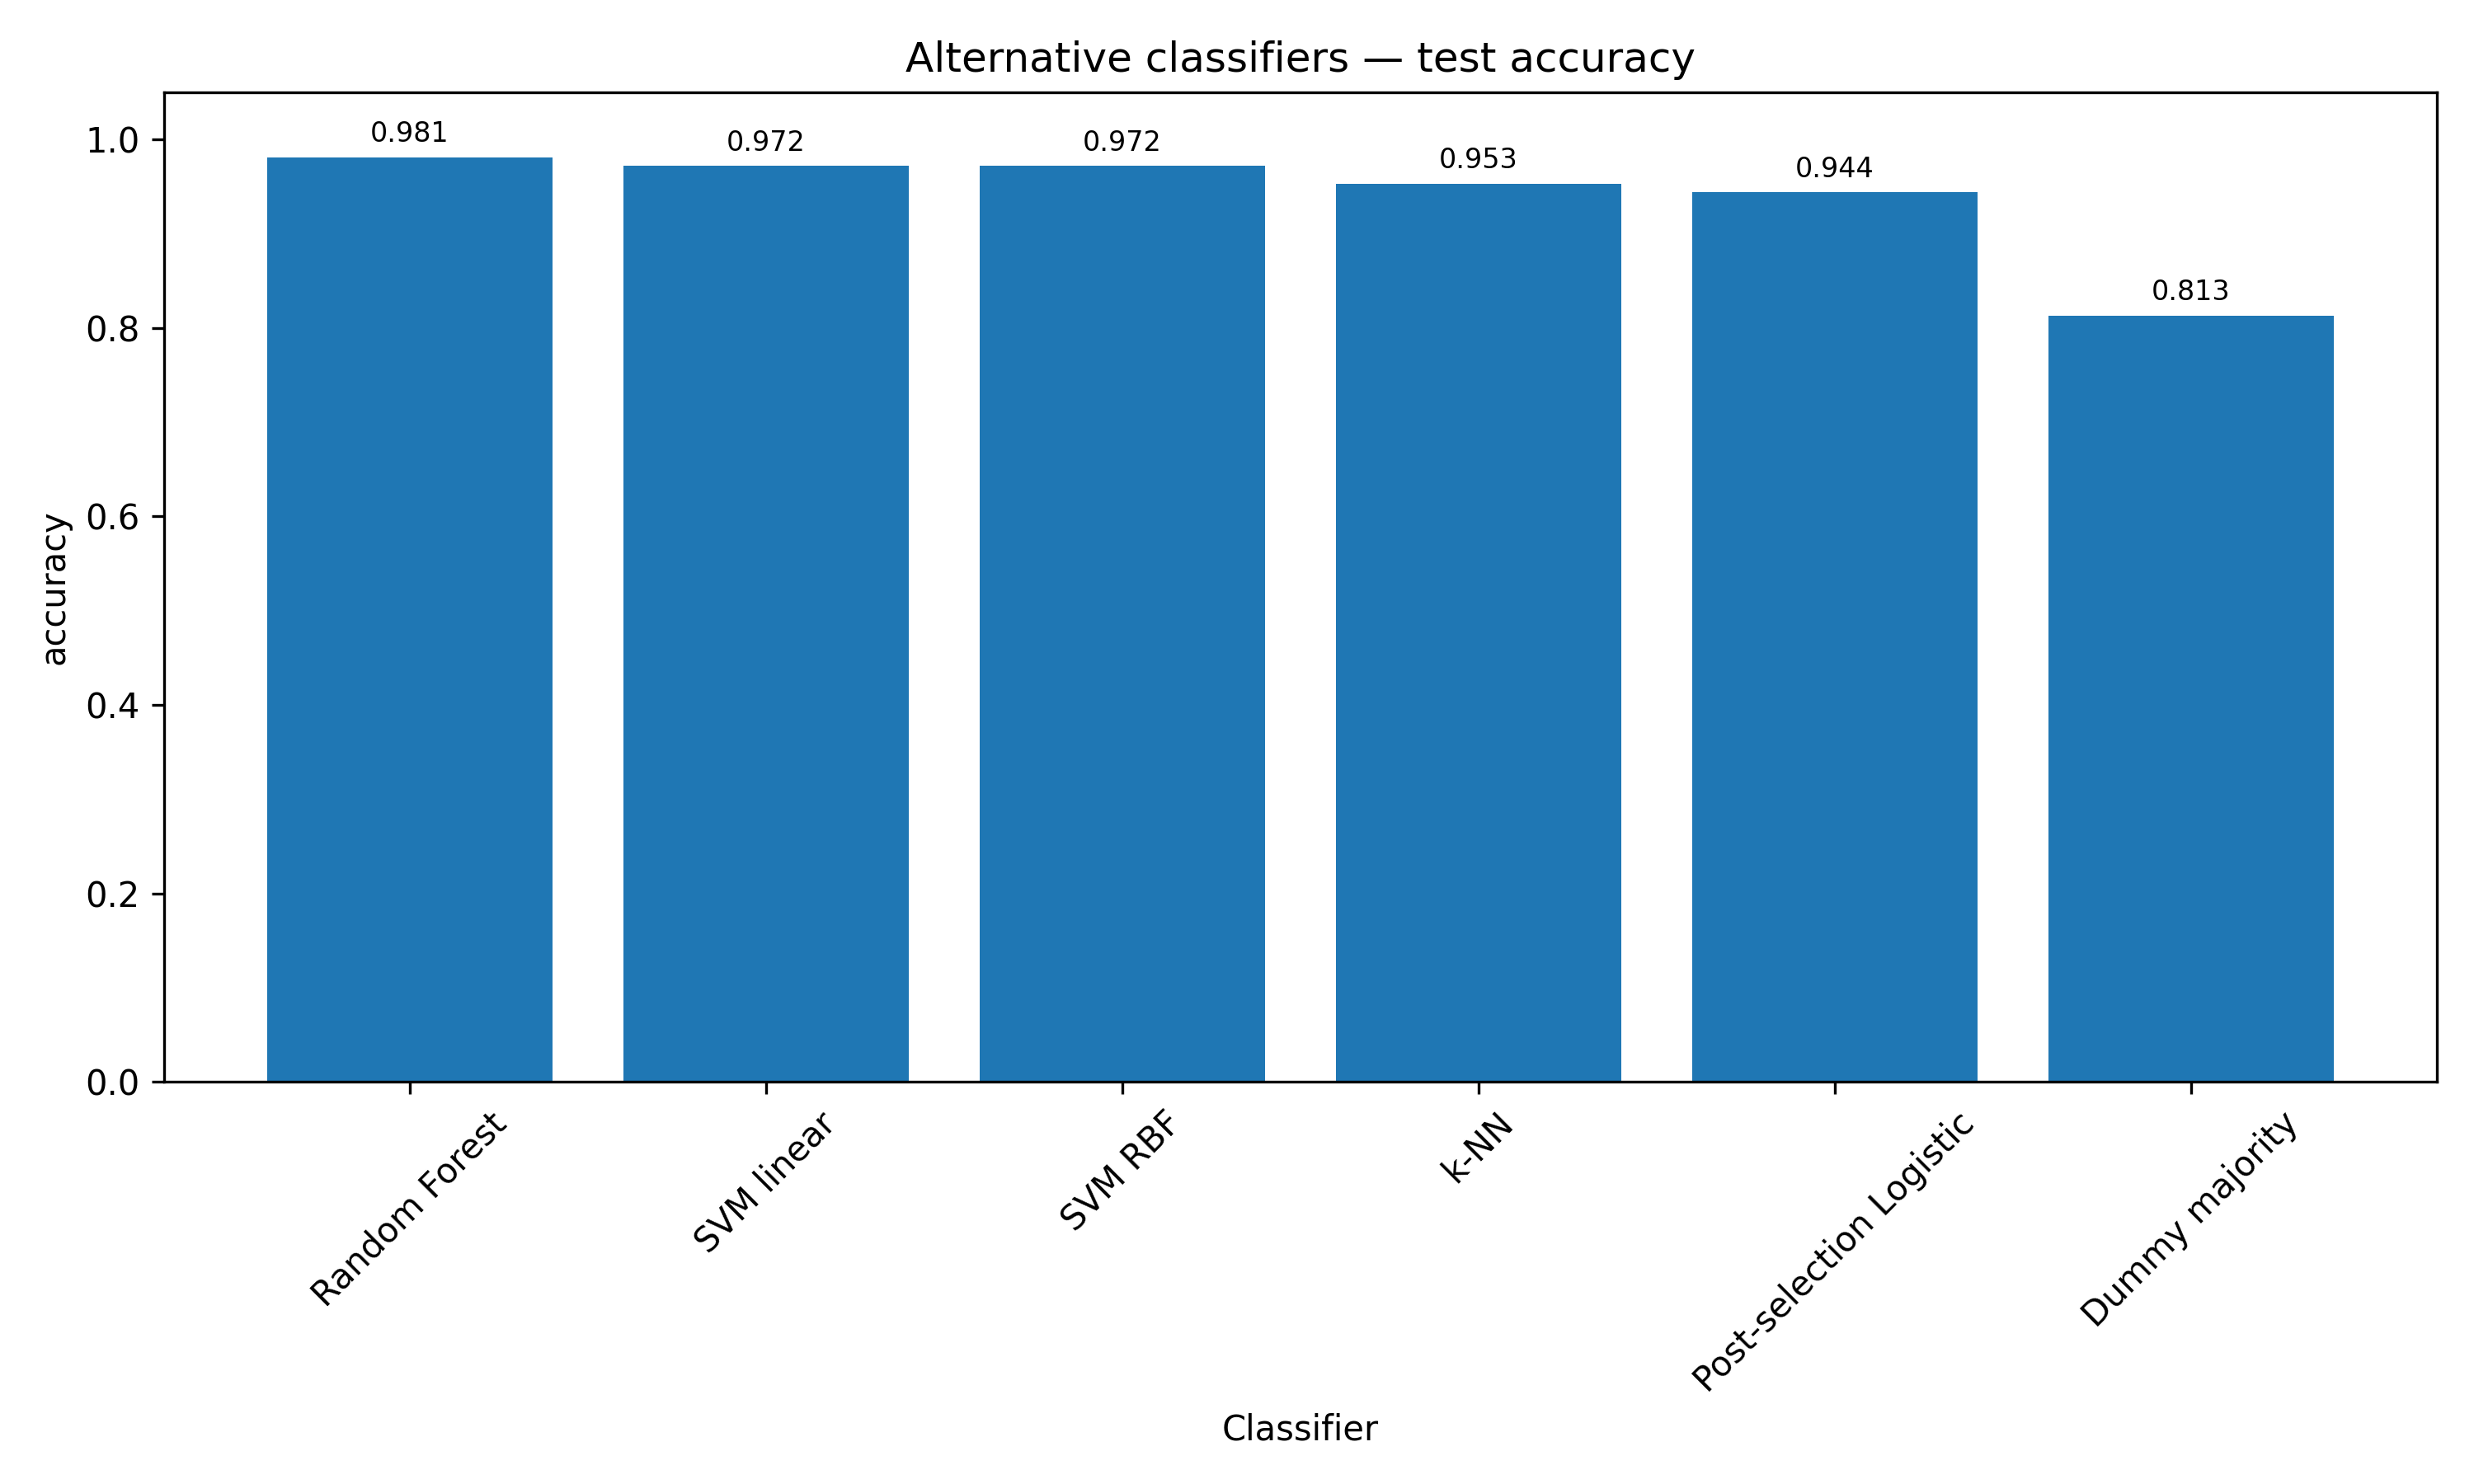
\includegraphics[width=0.7\textwidth]{alternative_classifiers_accuracy_comparison.png}
\caption{Accuracy comparison across models.}
\label{fig:phase5_acc}
\end{figure}

\begin{figure}[H]
\centering
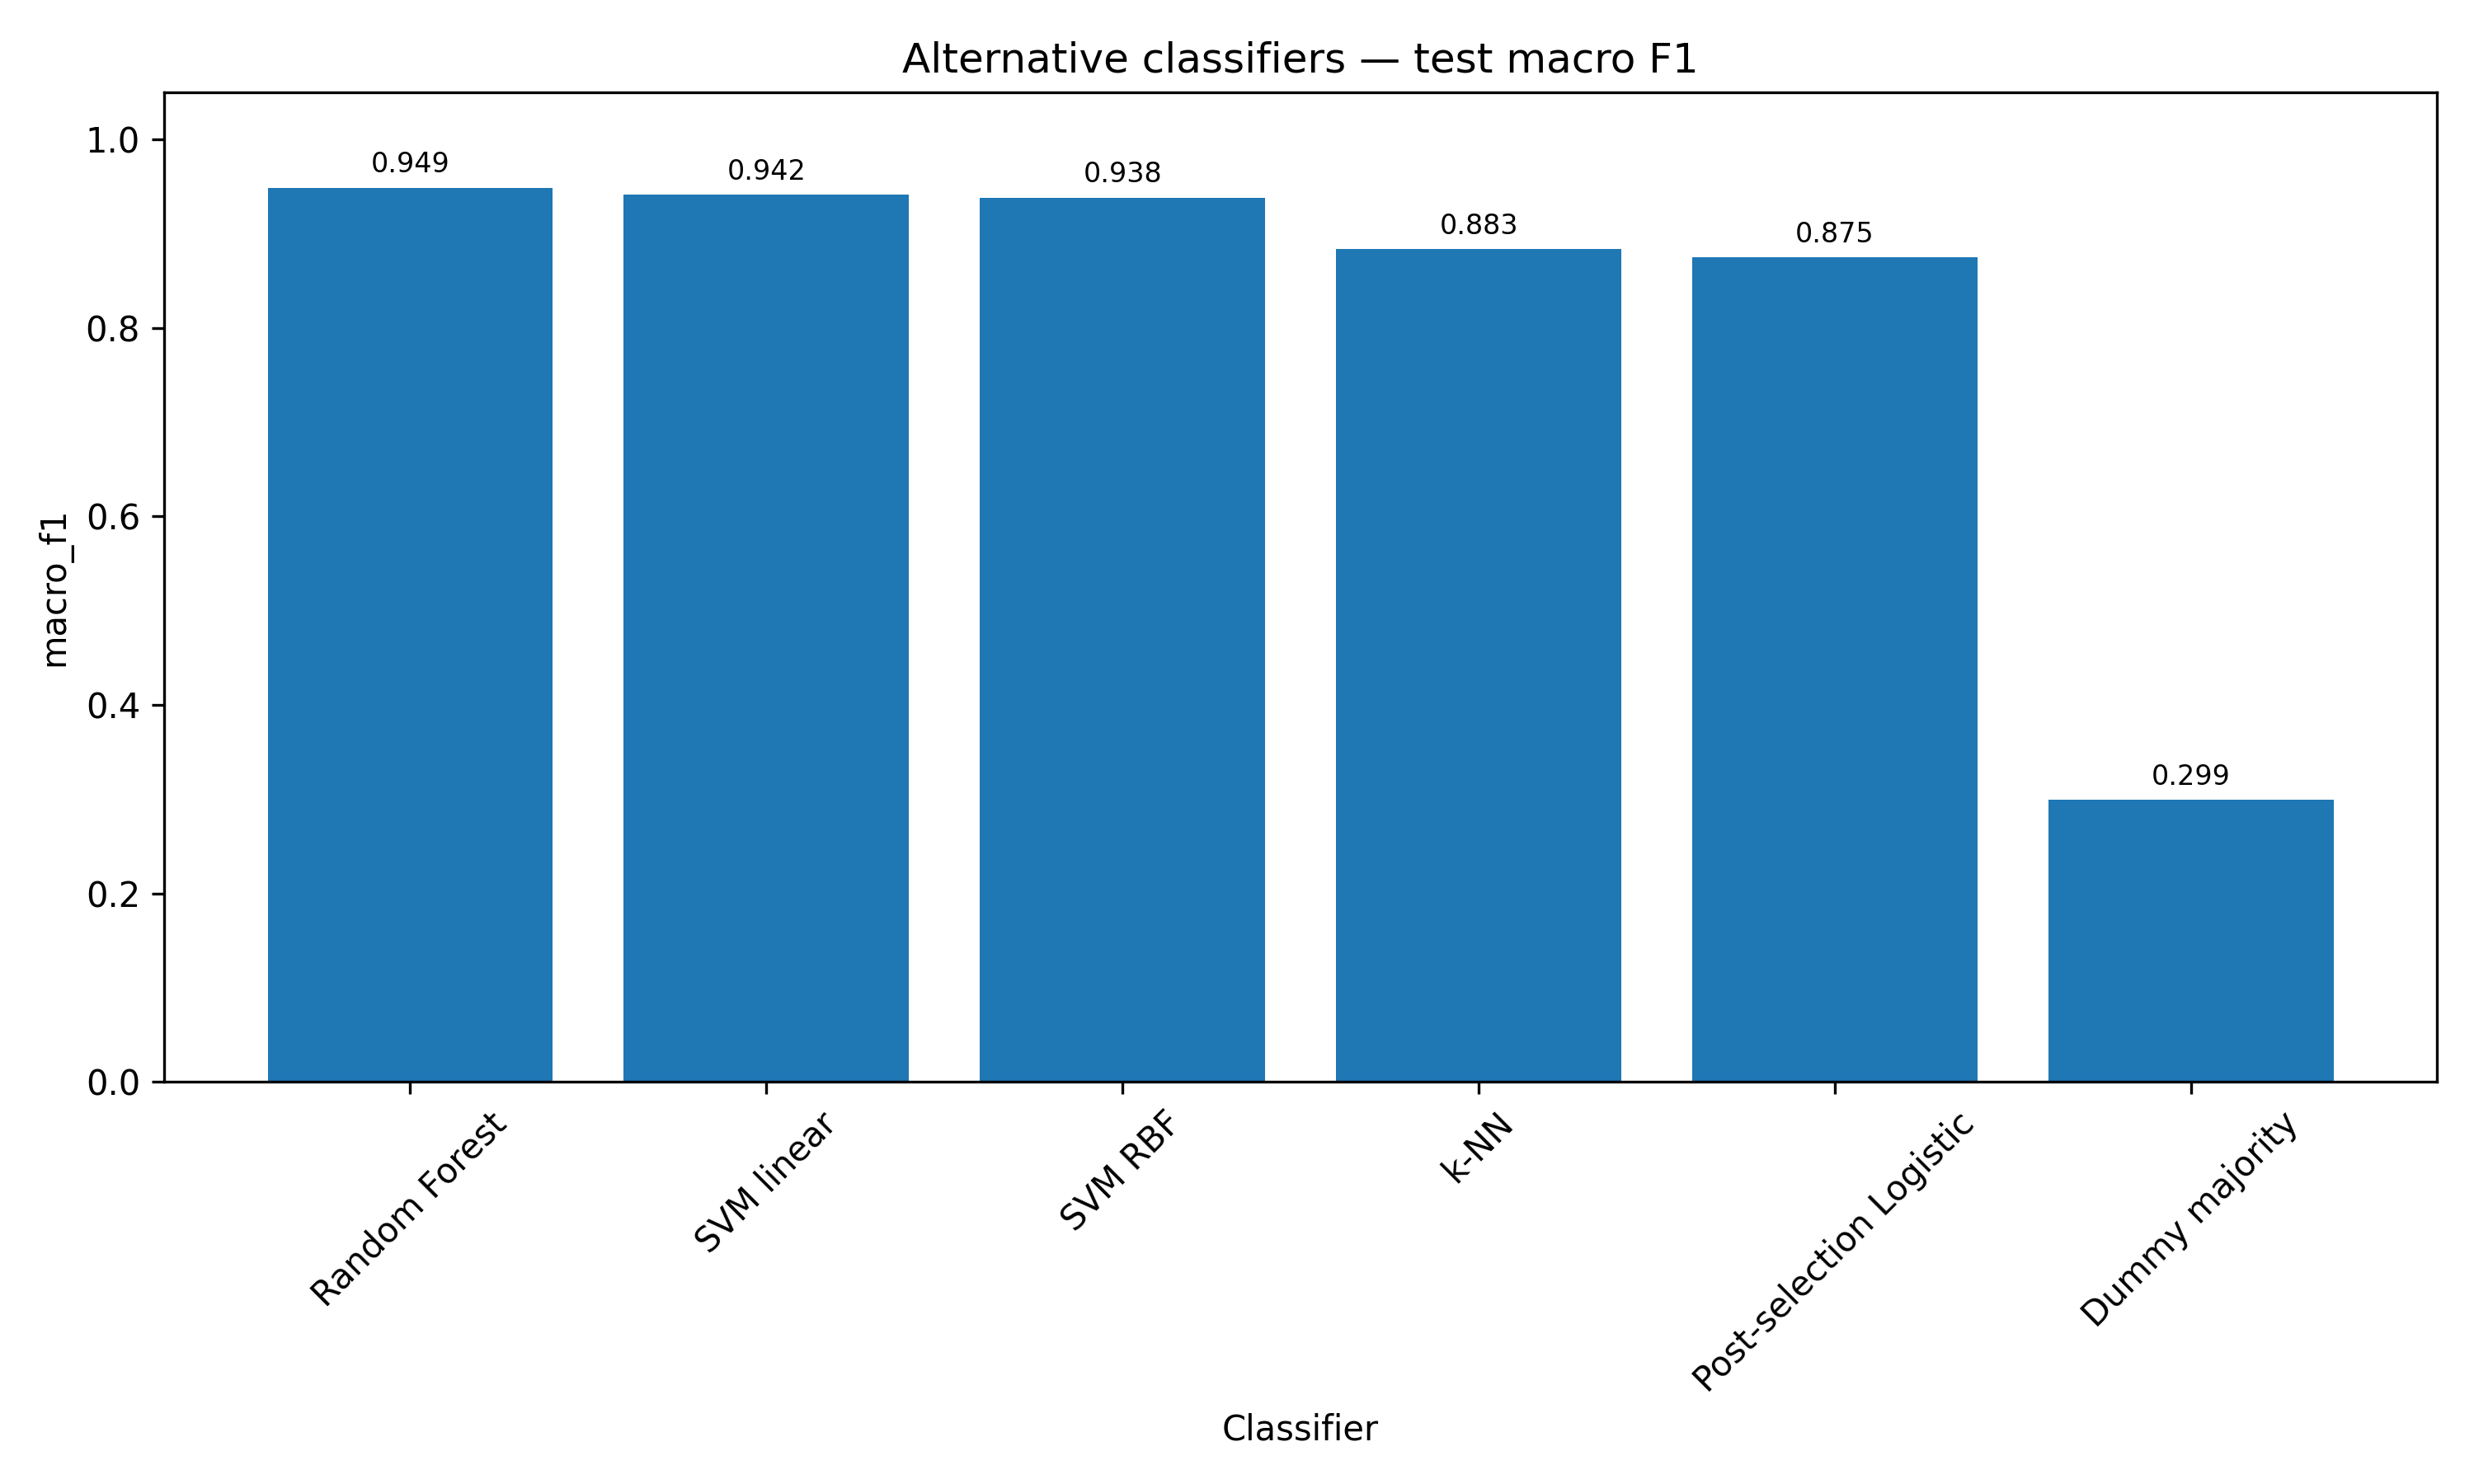
\includegraphics[width=0.7\textwidth]{alternative_classifiers_macro_f1_comparison.png}
\caption{Macro F1 comparison across models.}
\label{fig:phase5_f1}
\end{figure}

Random Forest achieves the best performance, improving macro F1 from 0.9229 to 0.9486. This indicates that non-linear interactions between features play a significant role.

\begin{figure}[H]
\centering
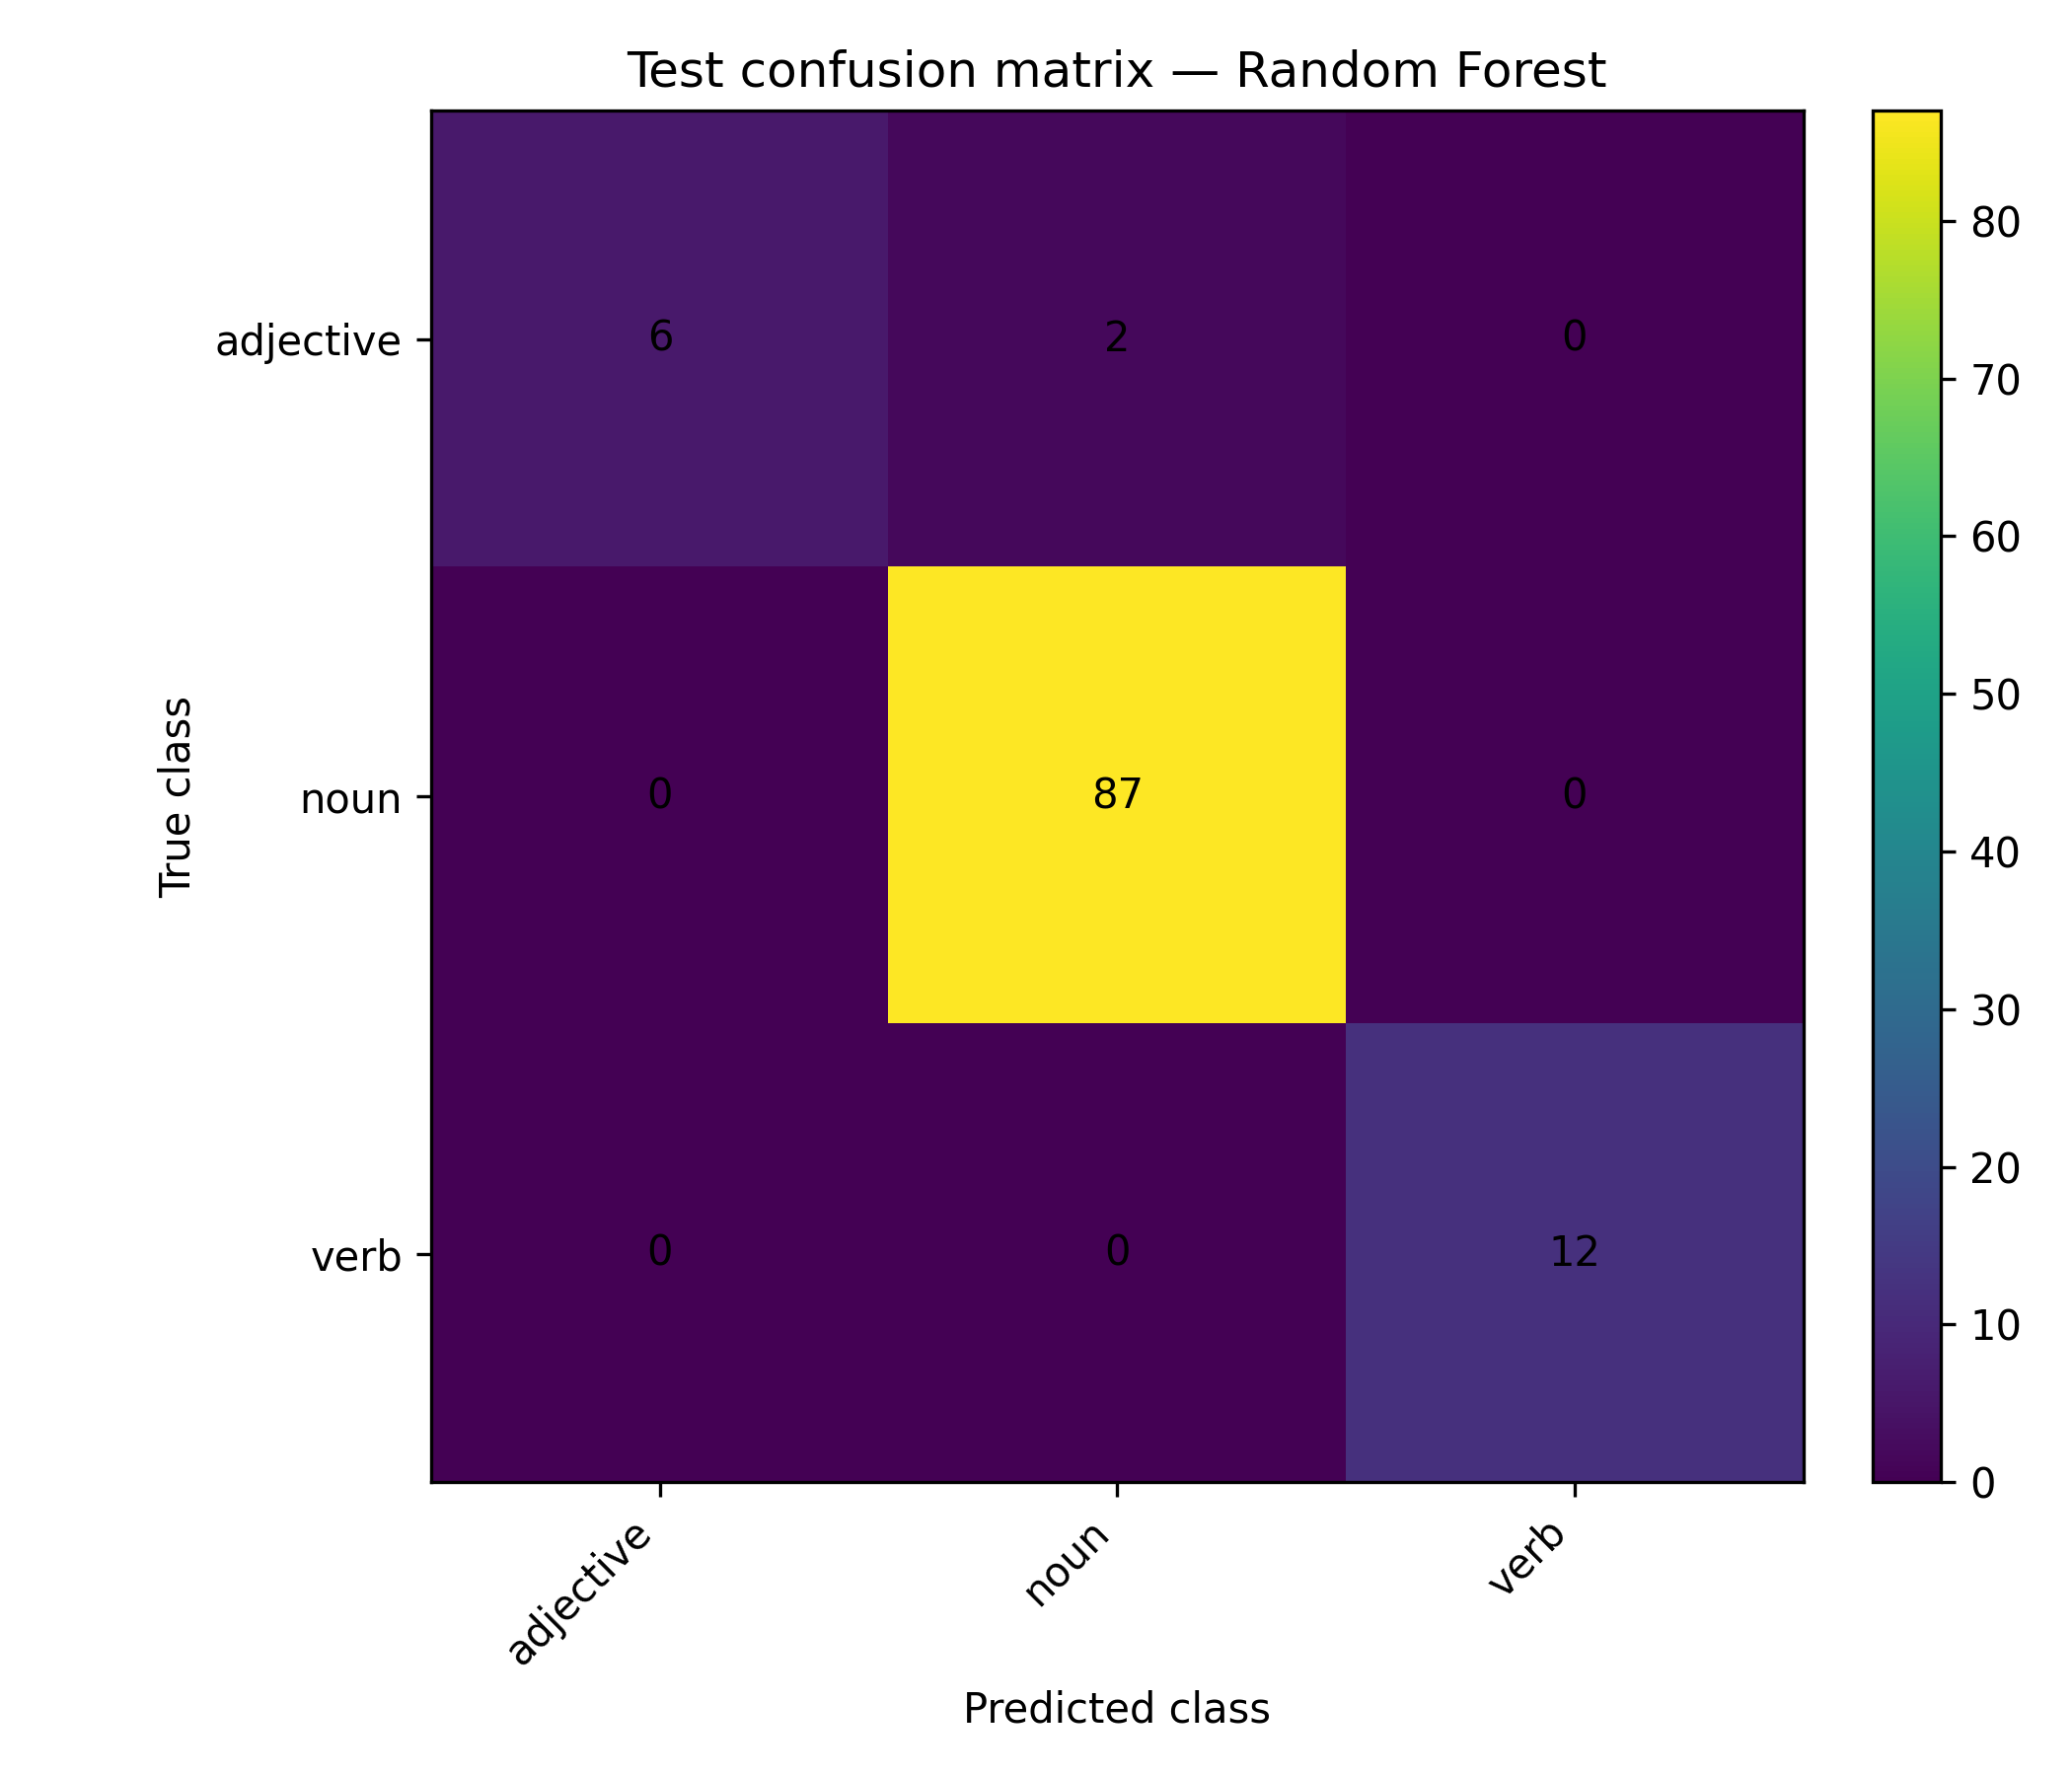
\includegraphics[width=0.6\textwidth]{random_forest_confusion_matrix_test.png}
\caption{Random Forest confusion matrix.}
\label{fig:phase5_rf}
\end{figure}

\paragraph{Conclusion}

The comparison highlights a key result: while linear models capture most of the signal, non-linear classifiers further improve performance by modeling interactions between features. This confirms that semantic representations are structured and that meaning emerges from combinations of attributes rather than isolated dimensions.
\subsection{VI. Final model comparison and interpretation}

This final phase integrates the results obtained across all previous analyses, with the objective of identifying the models that provide the best trade-off between predictive performance, statistical stability, and interpretability. The comparison includes the baseline multinomial logistic regression, the regularized models (LASSO and Elastic Net), the post-selection logistic model, and the alternative non-linear classifiers.
From a purely predictive perspective, the results clearly indicate that performance improves progressively along the pipeline. The baseline multinomial logistic model achieves an accuracy of 0.9533 and a macro F1-score of 0.8904. Regularization leads to consistent improvements, with Elastic Net reaching 0.9705 accuracy and 0.9200 macro F1. The post-selection model further refines these results, achieving 0.9720 accuracy and 0.9229 macro F1. Finally, the Random Forest classifier outperforms all linear approaches, reaching 0.9813 accuracy and 0.9486 macro F1.
These improvements are not marginal. The increase in macro F1 from 0.8904 to 0.9486 represents a substantial gain in balanced classification performance across all classes. This confirms that the successive methodological steps—regularization, feature selection, and non-linear modelling—are not only theoretically justified, but also empirically effective.
However, predictive performance alone is not sufficient to determine the best model. From the perspective of interpretability, multinomial logistic regression models remain superior. The LASSO and Elastic Net solutions provide sparse and stable representations of the semantic space, identifying a reduced subset of predictors that can be directly interpreted in terms of semantic dimensions. In contrast, Random Forest offers higher predictive accuracy but at the cost of reduced interpretability, since the decision process is distributed across many trees and interactions.
From a statistical learning perspective, the results also confirm the importance of controlling multicollinearity and dimensionality. The strong correlations observed among semantic features (22 pairs with $|r|\geq 0.8$ and 51 predictors with VIF $\geq 5$) make unregularized models unstable. Regularization and feature selection mitigate this issue by reducing variance and focusing the model on the most informative predictors.
Overall, the comparison suggests that no single model is universally optimal. Instead, the choice depends on the objective of the analysis. If the goal is interpretability and semantic insight, regularized multinomial models are preferable. If the goal is predictive accuracy, non-linear ensemble methods such as Random Forest provide the best results.

\vspace{0.5cm}

\section{Results}
\label{sec:results}

The empirical results of the project provide a coherent picture of the statistical properties of the Binder semantic feature space and its suitability for lexical-semantic classification.
First, the preprocessing phase confirms that the dataset is relatively clean but exhibits two important characteristics: moderate missingness and strong class imbalance. Missing values are concentrated in a small number of features and are successfully handled through median imputation, without loss of observations. The class distribution is highly skewed, with approximately 81\% of observations belonging to the class \emph{Thing}. This imbalance has direct consequences for model evaluation and motivates the use of metrics beyond simple accuracy.
Second, the unsupervised analysis reveals that the semantic feature space contains meaningful structure, but that this structure does not align directly with the target classes. PCA shows that the first two principal components explain approximately 36\% of the total variance, with a clear interpretation in terms of a concreteness–abstractness axis. Clustering methods identify coherent semantic groupings at a fine-grained level, but these clusters do not correspond strongly to the three lexical-semantic categories. This indicates that the semantic representation captures rich information, but not in a way that directly mirrors morphosyntactic classes.
Third, the supervised analysis demonstrates that the semantic features are highly informative for classification. Even the baseline multinomial logistic regression achieves high accuracy (0.9533), significantly above the trivial majority-class baseline (~0.811). However, the gap between accuracy and macro F1 reveals that performance is uneven across classes, with minority classes being harder to predict.
The introduction of regularization leads to consistent improvements. LASSO and Elastic Net increase both accuracy and macro F1, with Elastic Net providing the best balance. These results confirm that controlling multicollinearity improves generalization. Feature selection further enhances performance, showing that a reduced subset of predictors is sufficient to capture most of the relevant signal.
The high-dimensional expansion combined with feature screening demonstrates that increasing model complexity must be carefully controlled. While the expanded feature space allows the inclusion of non-linear effects and interactions, it also introduces noise and redundancy. Screening successfully reduces dimensionality, preserving the most informative predictors and stabilizing the subsequent models.
Finally, the comparison with alternative classifiers shows that non-linear models can further improve performance. Random Forest achieves the best results, with 0.9813 accuracy and 0.9486 macro F1, indicating that interactions between semantic features play a significant role in the classification task.
Overall, the results confirm that the Binder semantic representation is both informative and structured, but also redundant and partially non-linear. The combination of regularization, feature selection, and non-linear modelling provides the most effective strategy for exploiting this representation.

\vspace{0.5cm}

\section{Discussion}
\label{sec:discussion}

The findings of this project provide several insights into the nature of semantic representations and the challenges of statistical learning in this domain.
A first important observation is that semantic similarity and lexical classification are not equivalent problems. The unsupervised analysis shows that the feature space naturally organizes words into semantically coherent clusters, such as groups of animals, food items, or emotional concepts. However, these clusters do not align neatly with morphosyntactic categories. This suggests that lexical classes such as \emph{Thing}, \emph{Action}, and \emph{Property} are not simply reflections of the geometry of the semantic space, but rather more abstract linguistic constructs.
A second key result concerns the role of multicollinearity. The strong correlations observed among semantic features are not a technical artifact, but a fundamental property of the representation. Many experiential dimensions are conceptually related and tend to co-occur. From a statistical perspective, this creates instability in model estimation and makes feature selection more challenging. The effectiveness of Elastic Net compared to LASSO alone highlights the importance of accounting for correlated predictors rather than selecting them independently.
A third insight relates to the distributed nature of semantic information. The fact that good classification performance can be achieved using a reduced subset of features indicates that not all dimensions are equally informative. At the same time, the superiority of non-linear models suggests that the predictive signal is not concentrated in individual features, but rather in their interactions. This supports the view that word meaning emerges from combinations of semantic attributes rather than from isolated dimensions.
The comparison between linear and non-linear models also illustrates a fundamental trade-off in statistical learning. Linear models offer interpretability and theoretical clarity, making them suitable for understanding which features matter. Non-linear models, on the other hand, provide higher predictive accuracy but are more difficult to interpret. In this project, both perspectives are necessary: linear models for interpretation, and non-linear models for performance.
Finally, the high-dimensional extension of the feature space highlights the risks and opportunities of increasing model complexity. While adding interaction terms can potentially capture richer semantic patterns, it also increases noise and overfitting risk. The success of feature screening demonstrates that dimensionality reduction is essential in such settings, acting as a bridge between expressiveness and stability.

\vspace{0.5cm}

\section{Conclusion}
\label{sec:conclusion}

This project has reformulated the analysis of the Binder semantic dataset within the framework of high-dimensional statistical learning. Starting from a cognitively motivated representation of word meaning, we have developed a structured pipeline combining preprocessing, unsupervised exploration, supervised classification, multicollinearity diagnostics, feature screening, regularization, and model comparison.
The results show that the semantic feature space is highly informative for lexical classification, even when using simple linear models. However, the presence of strong correlations and redundancy requires the use of regularization techniques to obtain stable and interpretable models. Feature selection further improves performance by identifying a reduced subset of relevant predictors.
The extension to high-dimensional representations reveals that non-linear effects and interactions between semantic features play an important role. This is confirmed by the superior performance of Random Forest, which captures complex dependencies that linear models cannot fully represent.
From a broader perspective, the project highlights the importance of combining different methodological tools. Unsupervised learning provides insight into the structure of the semantic space, supervised learning quantifies predictive performance, and regularization and screening ensure stability in high-dimensional settings. Together, these approaches offer a comprehensive framework for analysing semantic data.
Future work could extend this analysis in several directions. Larger and more balanced datasets would allow more robust evaluation of minority classes. Alternative representations, such as distributional or contextual embeddings, could be compared with the Binder semantic features. Finally, more advanced models, including deep learning approaches, could be explored to further investigate the interaction between semantic structure and predictive performance.
In conclusion, the Binder semantic representation proves to be a rich and informative basis for statistical learning. When combined with appropriate modelling strategies, it allows both accurate prediction of lexical classes and meaningful interpretation of the underlying semantic dimensions.
\newpage

\addcontentsline{toc}{section}{References}
\printbibliography

\newpage

\appendix
\appendix
\section{Original clustering and biclustering analyses}
Testa's original project included an extensive exploratory unsupervised analysis of the Binder semantic feature space. The aim of this part of the work was not to predict lexical classes directly, but to investigate whether the 65 primitive semantic attributes were able to produce interpretable similarity structures among words. In other terms, Testa used unsupervised learning to address the question of whether lexical items that are semantically close in an intuitive sense also appear close when represented through Binder et al.'s componential semantic ratings.
The first method applied was k-means clustering. This algorithm partitions the observations into \(k\) groups by minimizing the within-cluster sum of squared distances, so that words assigned to the same cluster are expected to have similar semantic profiles. The method was used as an initial exploratory baseline because it is simple, widely used, and provides a direct way to test whether the semantic feature space naturally separates into distinct groups. Before fixing the number of clusters, Testa evaluated different criteria, including within-cluster dissimilarity, the Hartigan index, and the average silhouette score. These diagnostics initially suggested \(k = 2\) as a possible solution, but the corresponding partition was too coarse and did not lead to a clear semantic interpretation. A second configuration with \(k = 10\) was therefore examined. Although this larger number of clusters began to reveal some semantic organization, the resulting groups remained relatively noisy and difficult to interpret. This indicated that the original 65-dimensional space contained meaningful information, but that k-means was not sufficiently flexible to recover stable semantic categories from it.
The limitations of k-means motivated the use of agglomerative hierarchical clustering. Hierarchical clustering was chosen because, unlike k-means, it does not require a single fixed partition to be imposed from the beginning. Instead, it builds a dendrogram representing nested similarity relations among observations, which can then be cut at different levels of granularity. In Testa's original project, an agglomerative approach with complete linkage was used. Complete linkage defines the distance between two clusters according to the maximum distance between their members, and therefore tends to produce relatively compact clusters. As in the k-means analysis, the dendrogram was cut at \(k = 2\) and \(k = 10\). The two-cluster solution again proved too generic, whereas the ten-cluster solution produced more interpretable semantic groupings. In particular, some clusters could be associated with broad semantic areas such as food, animals, natural events, musical instruments, and sentiment-related words. This result suggested that the semantic ratings did encode meaningful similarity relations, but also that the structure of the original feature space was not sharply separated into clean clusters.
A further step was the application of biclustering. This method was introduced because standard clustering groups either observations or variables, whereas biclustering simultaneously clusters rows and columns of a data matrix. This is especially relevant for semantic feature data: two words may be similar only with respect to a specific subset of semantic dimensions, rather than across all 65 features. For example, a group of words may be close in auditory features but not in visual or social features. Biclustering is therefore better suited to identifying local semantic patterns, where subsets of lexical items are associated with subsets of experiential attributes. In Testa's original project, biclustering was performed using the \texttt{isa2} package in R, based on the Iterative Signature Algorithm. Among the biclustering approaches tested, this method produced the most coherent semantic output.
The biclustering analysis identified a large number of local structures. Testa reported 199 biclusters, many of which were semantically interpretable both in terms of the words grouped together and in terms of the features involved. The eight most relevant or coherent biclusters were manually interpreted as corresponding to semantic domains such as \emph{Time}, \emph{Food and Drinks}, \emph{Animals}, \emph{Sounds}, \emph{Locations}, \emph{Negative Events and Feelings}, \emph{Human Beings} and \emph{Practical Tools}. This result was important because it showed that the Binder feature matrix contains local semantic regularities: groups of words are not only similar globally, but can share specific subsets of experiential dimensions. At the same time, the analysis also revealed substantial overlap among biclusters, meaning that the same lexical item could belong to multiple semantic patterns. This overlap is not necessarily a weakness; rather, it reflects the fact that word meaning is multidimensional and that a single concept can participate in different semantic domains.
After these first clustering attempts, Testa introduced Principal Component Analysis as a denoising and dimensionality reduction step. The rationale was that the original semantic space is high enough in dimension to contain redundancy, correlated predictors, and noise. PCA transforms the original variables into orthogonal linear combinations, ordered by the amount of variance they explain. By projecting the data onto a smaller number of principal components, it becomes possible to retain the dominant structure of the dataset while reducing the influence of less informative variation. In Testa's analysis, the first ten principal components were reported to explain approximately 80\% of the total variance, with the first few components carrying the largest share of information.
The PCA loadings were then inspected to understand the semantic meaning of the main components. In particular, the first two principal components were visualized through a correlation circle and feature contribution plots. Testa interpreted these two components as reflecting two broad and opposite latent semantic dimensions. One component was mainly associated with temporal, causal, social, emotional and attentional features, and was interpreted as closer to an abstract semantic dimension. The other component was more strongly associated with sensory-motor and spatial features, and was interpreted as closer to a concrete semantic dimension. This observation led to one of the main qualitative conclusions of the original project: the opposition between \emph{Concreteness} and \emph{Abstractness} may represent an important latent structure in the semantic organization of the dataset.
PCA was also used as a preprocessing step before repeating the clustering analysis. The reason for doing this was that clustering in the original feature space may be affected by redundancy and multicollinearity, while clustering in a lower-dimensional PCA space may reveal cleaner groupings. Testa therefore applied k-means and hierarchical clustering to the PCA-reduced representation. Hierarchical clustering again produced the most meaningful results. With \(k = 2\), the clusters approximately separated abstract from concrete lexical items. With larger values of \(k\), especially between \(k = 10\) and \(k = 28\), the clusters became more semantically specific and closer to the semantic macro-categories identified in Binder et al.'s dataset. However, this increase in semantic detail came with a reduction in the average silhouette score. Testa therefore interpreted the range between 10 and 28 clusters as a trade-off between quantitative cluster compactness and qualitative semantic interpretability.
Overall, the unsupervised analyses in Testa's original project had three main purposes. First, they served as a validation of the Binder semantic feature representation, showing that the 65 experiential attributes were not arbitrary but contained recoverable similarity structures. Second, they provided exploratory evidence that some semantic domains could be identified from the data without using lexical-class labels. Third, they motivated the later supervised analysis by showing that the semantic feature space already contained structure relevant to lexical organization. Among the methods tested, simple k-means was the least successful, hierarchical clustering was more interpretable, PCA improved the clarity of the cluster structure, and biclustering provided the richest local semantic patterns.
In the present work, these analyses are reported only as background and exploratory evidence. They are not part of the main methodological contribution, because the focus is shifted from unsupervised semantic grouping to supervised high-dimensional statistical learning. Nevertheless, they remain relevant because they justify the use of the Binder feature space as a meaningful input representation. Testa's original project showed that the semantic ratings contain interpretable structure; the present project starts from that result and asks a different question, namely how regularization, feature screening, rebalancing and stability analysis behave when this semantic representation is expanded into a large-feature-space classification problem.

\section{Detailed explanation of the Python preprocessing pipeline}

This appendix describes in detail the three Python scripts used to implement the preprocessing phase of the project. The scripts correspond to the first three operational steps of the analysis pipeline and are stored as separate modules in order to keep the workflow transparent, reproducible, and easy to inspect. The three scripts are:

\begin{itemize}
    \item \texttt{dataset\_initial\_cleaning.py}, corresponding to Phase 1.1;
    \item \texttt{dataset\_train\_test\_split.py}, corresponding to Phase 1.2;
    \item \texttt{dataset\_imputation\_scaling.py}, corresponding to Phase 1.3.
\end{itemize}

The overall objective of these scripts is not to fit predictive models, but to construct a reliable analytical dataset. For this reason, the preprocessing pipeline is deliberately separated from the modelling pipeline. In particular, the scripts avoid performing operations that could introduce data leakage, such as imputing missing values or estimating scaling parameters before the train--test split. Each phase saves its own outputs inside the \texttt{outputs/I/} directory, so that the intermediate results can be examined and reused by later phases of the project.

\subsection{Phase 1.1: Initial dataset cleaning}

The first script, \texttt{dataset\_initial\_cleaning.py}, performs the initial structural inspection and cleaning of the 65-feature semantic dataset. The input file is:

\begin{center}
\texttt{dataset/slld\_binder\_Xy\_65\_features.csv}
\end{center}

The script saves its outputs in:

\begin{center}
\texttt{outputs/I/phase1\_1\_initial\_cleaning/}
\end{center}

This phase is intentionally conservative. Its purpose is not to transform the data statistically, but to verify that the dataset has the expected structure and to produce a clean raw version of the data that can be safely used in later phases.

\subsubsection{Path definition and output organization}

At the beginning of the script, the input and output paths are defined using the \texttt{Path} class from Python's \texttt{pathlib} module. This makes the code more readable and more robust than relying on raw string paths.

The script defines the main dataset directory:

\begin{center}
\texttt{DATASET\_DIR = Path("./dataset")}
\end{center}

and the output directory:

\begin{center}
\texttt{OUTPUT\_DIR = Path("./outputs/I//phase1\_1\_initial\_cleaning")}
\end{center}

The double slash in \texttt{I//phase1\_1\_initial\_cleaning} does not change the semantic meaning of the path: operating systems normalize it automatically. The important point is that all outputs from Phase 1.1 are stored inside the folder \texttt{outputs/I/}, which identifies the first main block of the project pipeline.

The script produces five files:

\begin{itemize}
    \item \texttt{slld\_phase1\_1\_clean\_raw.csv}, the structurally cleaned raw dataset;
    \item \texttt{missing\_values\_report.csv}, a report on missing values by feature;
    \item \texttt{duplicated\_word\_forms.csv}, a report on repeated word forms;
    \item \texttt{target\_class\_distribution.csv}, a report on class frequencies;
    \item \texttt{phase1\_1\_summary.json}, a machine-readable summary of the phase.
\end{itemize}

The presence of both CSV reports and a JSON summary is useful because the CSV files are easy to inspect manually, while the JSON file can be automatically read by later scripts or used for reproducibility checks.

\subsubsection{Expected columns and target validation}

The script expects three non-feature columns:

\begin{center}
\texttt{entry\_id}, \texttt{word}, \texttt{target\_word\_class}
\end{center}

These columns are stored in the list:

\begin{center}
\texttt{ID\_COLS = ["entry\_id", "word", "target\_word\_class"]}
\end{center}

All remaining columns are treated as semantic feature columns. Since the dataset is expected to contain 65 semantic predictors, the script checks whether exactly 65 feature columns are detected. If the number is different from 65, the script does not immediately stop, but prints a warning. This is a sensible choice because a mismatch in the number of predictors may indicate that the wrong input file has been loaded, but it does not necessarily mean that the file is unreadable.

The script also defines the valid target classes as:

\begin{center}
\texttt{\{"noun", "verb", "adjective"\}}
\end{center}

This check is essential because the whole supervised part of the project assumes a three-class classification task. Rows whose target label is not included in this set are treated as structurally invalid. If such rows are found, the script prints them and removes them. In the prepared dataset, this step is expected to remove no observations.

\subsubsection{Loading the dataset and checking file existence}

Before loading the dataset, the script checks whether the input file exists. If the file is missing, it raises a \texttt{FileNotFoundError}. This is preferable to letting \texttt{pandas} fail later with a less informative error message.

The dataset is then loaded using:

\begin{center}
\texttt{pd.read\_csv(INPUT\_FILE)}
\end{center}

After loading, the script prints the number of rows and columns. This immediate diagnostic is useful because it allows us to verify that the expected dataset has been loaded before any cleaning operation is applied.

\subsubsection{Textual cleaning of word and target columns}

The script performs a minimal cleaning of the textual columns \texttt{word} and \texttt{target\_word\_class}. Specifically, it converts the values to strings and removes accidental leading or trailing whitespace:

\begin{center}
\texttt{astype(str).str.strip()}
\end{center}

This operation is deliberately limited. The script does not lowercase the words, does not lemmatize them, and does not modify their lexical content. This is important because the lexical item is part of the dataset identity. The preprocessing phase should not alter linguistic information unless there is a clear methodological justification.

\subsubsection{Exact duplicate rows}

The script then checks for exact duplicate rows using:

\begin{center}
\texttt{df.duplicated().sum()}
\end{center}

Exact duplicates are rows that are identical across all columns. If such rows are present, they are removed with:

\begin{center}
\texttt{df.drop\_duplicates()}
\end{center}

This choice is methodologically safe because exact duplicates do not introduce new information. Keeping them would artificially increase the weight of repeated observations in later analyses.

It is important to distinguish exact duplicate rows from duplicated word forms. Exact duplicate rows are redundant observations; duplicated word forms may instead correspond to legitimate lexical entries.

\subsubsection{Duplicated word forms}

After removing exact duplicates, the script searches for duplicated values in the \texttt{word} column:

\begin{center}
\texttt{df\_clean.duplicated("word", keep=False)}
\end{center}

The result is sorted by word and target class and saved to:

\begin{center}
\texttt{duplicated\_word\_forms.csv}
\end{center}

Duplicated word forms are reported but not removed. This is a crucial methodological decision. The statistical unit of this project is not simply the written word form, but the lexical entry. Therefore, the same orthographic word can be validly represented more than once if it corresponds to different lexical-semantic roles. For instance, a word may occur once as a verb and once as an adjective. Removing one of these entries would incorrectly collapse distinct lexical uses.

\subsubsection{Missing-value analysis}

The script computes missing values only on the feature columns, not on the identifier columns. For each semantic feature, it calculates:

\begin{itemize}
    \item the number of missing values;
    \item the percentage of missing values.
\end{itemize}

The missing-value report is sorted in descending order, so that the most problematic features appear first. The report is saved as:

\begin{center}
\texttt{missing\_values\_report.csv}
\end{center}

The script also computes:

\begin{itemize}
    \item the number of rows with at least one missing value;
    \item the number of complete rows.
\end{itemize}

This information is important because it quantifies the cost of complete-case analysis. If rows with missing values were removed immediately, the sample size would decrease. Since the dataset is small and class-imbalanced, aggressive deletion would be statistically undesirable.

For this reason, Phase 1.1 does not impute missing values and does not remove incomplete rows. Missing values are only described and preserved for later treatment.

\subsubsection{Class distribution}

The script computes the distribution of \texttt{target\_word\_class} using:

\begin{center}
\texttt{value\_counts()}
\end{center}

It then converts the counts into percentages and saves the output to:

\begin{center}
\texttt{target\_class\_distribution.csv}
\end{center}

This step is essential because the target distribution determines how model performance must be interpreted. If one class is much more frequent than the others, raw accuracy can be misleading. A classifier can obtain high accuracy simply by predicting the majority class. Therefore, the class distribution report produced in Phase 1.1 motivates the use of balanced accuracy, macro-F1, class-wise recall, and confusion matrices in later phases.

\subsubsection{Saving the clean raw dataset}

At the end of the script, the cleaned dataset is saved as:

\begin{center}
\texttt{slld\_phase1\_1\_clean\_raw.csv}
\end{center}

This file is called \emph{clean raw} because it is structurally cleaned but not statistically transformed. In particular, the script explicitly avoids:

\begin{itemize}
    \item removing rows with missing values;
    \item removing columns with missing values;
    \item imputing missing values;
    \item standardizing features;
    \item performing a train--test split.
\end{itemize}

This design is methodologically correct because imputation and scaling must be performed after the train--test split, and they must be fitted only on the training set.

\subsubsection{Summary JSON}

Finally, the script saves a JSON file containing the main numerical information and methodological decisions of Phase 1.1. The JSON summary includes:

\begin{itemize}
    \item input and output file paths;
    \item initial and cleaned dataset dimensions;
    \item number of identifier columns and feature columns;
    \item valid target classes;
    \item number of exact duplicates removed;
    \item number of duplicated word-form rows;
    \item number of rows with missing values;
    \item list of columns with missing values;
    \item explicit methodological decisions.
\end{itemize}

This JSON file makes the preprocessing phase auditable. Instead of relying only on the printed console output, the project stores a structured summary that can be inspected later.

\subsubsection{Pseudocode for Phase 1.1}

\begin{algorithm}[H]
\caption{Phase 1.1: Initial dataset cleaning}
\begin{algorithmic}[1]
\State Define input and output paths
\State Create output directory if it does not exist
\State Load the 65-feature dataset
\State Check that required columns are present
\State Identify feature columns as all non-identifier columns
\If{number of feature columns is not 65}
    \State Print warning
\EndIf
\State Strip accidental whitespace from \texttt{word} and \texttt{target\_word\_class}
\State Check that all target labels are valid
\If{invalid target labels are found}
    \State Remove invalid rows
\EndIf
\State Count exact duplicate rows
\State Remove exact duplicate rows
\State Identify duplicated word forms
\State Save duplicated word-form report
\State Compute missing-value counts and percentages by feature
\State Save missing-value report
\State Compute target class distribution
\State Save target class distribution report
\State Save structurally cleaned raw dataset
\State Save JSON summary of the phase
\end{algorithmic}
\end{algorithm}

\subsection{Phase 1.2: Stratified train--test split}

The second script, \texttt{dataset\_train\_test\_split.py}, loads the structurally cleaned raw dataset produced in Phase 1.1 and creates a reproducible train--test split. Its input file is:

\begin{center}
\texttt{outputs/I/phase1\_1\_initial\_cleaning/slld\_phase1\_1\_clean\_raw.csv}
\end{center}

The outputs are saved in:

\begin{center}
\texttt{outputs/I/phase1\_2\_train\_test\_split/}
\end{center}

This phase is crucial because all later preprocessing operations must be fitted only on the training set. Therefore, the split is performed before imputation and before standardization.

\subsubsection{Purpose of the split}

The script separates the data into:

\begin{itemize}
    \item a training set, used to estimate preprocessing parameters and fit models;
    \item a test set, used only for external evaluation.
\end{itemize}

The split is stratified by the target variable \texttt{target\_word\_class}. Stratification is necessary because the dataset is strongly class-imbalanced. Without stratification, the random split could allocate too few verbs or adjectives to the test set, making evaluation unstable and potentially misleading.

\subsubsection{Configuration}

The script defines the following main configuration parameters:

\begin{itemize}
    \item \texttt{TEST\_SIZE = 0.20}, meaning that 20\% of the observations are assigned to the test set;
    \item \texttt{RANDOM\_STATE = 42}, ensuring reproducibility;
    \item \texttt{TARGET\_COL = "target\_word\_class"}, defining the stratification variable.
\end{itemize}

The use of a fixed random state is important because it guarantees that the same train--test split can be reproduced in future runs. Reproducibility is particularly important in a small and imbalanced dataset, where different splits could lead to noticeably different model performance.

\subsubsection{Helper function for class distribution}

The function:

\begin{center}
\texttt{compute\_class\_distribution(df, split\_name)}
\end{center}

computes, for a given dataset split:

\begin{itemize}
    \item the count of each class;
    \item the percentage of each class;
    \item the name of the split to which the report refers.
\end{itemize}

The function returns a \texttt{pandas} DataFrame. This design avoids repeated code and ensures that the class distributions for the full dataset, training set, and test set are computed in the same way.

\subsubsection{Helper function for missing values by split}

The function:

\begin{center}
\texttt{compute\_missing\_summary(df, feature\_cols, split\_name)}
\end{center}

computes missing-value counts and percentages for each feature within a given split. This is important because missingness may not be distributed identically between the training and test sets. By saving missing-value reports after the split, the project can verify how many missing values will have to be handled in each subset.

\subsubsection{Structural checks}

After loading the cleaned raw dataset, the script repeats some structural checks:

\begin{itemize}
    \item it verifies that the identifier columns are present;
    \item it checks that all target labels are valid;
    \item it identifies the feature columns;
    \item it checks whether 65 feature columns are detected.
\end{itemize}

Repeating these checks is not redundant. Since Phase 1.2 depends on the output of Phase 1.1, these checks ensure that the correct file has been loaded and that the file has not been modified accidentally.

\subsubsection{Minimum class-count check}

Before performing the stratified split, the script calculates the minimum class count:

\begin{center}
\texttt{df[TARGET\_COL].value\_counts().min()}
\end{center}

If any class has fewer than two observations, a stratified train--test split would not be feasible. The script therefore raises an error in this case. This is a defensive programming choice: it prevents the procedure from silently producing an invalid split.

\subsubsection{Stratified train--test split}

The split is performed using \texttt{train\_test\_split} from \texttt{sklearn.model\_selection}. The key argument is:

\begin{center}
\texttt{stratify=df[TARGET\_COL]}
\end{center}

This ensures that the relative class frequencies in the training and test sets remain close to those in the full dataset.

The script uses:

\begin{center}
\texttt{shuffle=True}
\end{center}

so that observations are randomly assigned to train and test while preserving class proportions.

After splitting, both datasets are sorted by \texttt{entry\_id}. This sorting does not affect the statistical content of the split, but improves readability and makes saved files easier to inspect.

\subsubsection{Saving raw train and test datasets}

The script saves:

\begin{itemize}
    \item \texttt{slld\_phase1\_2\_train\_raw.csv};
    \item \texttt{slld\_phase1\_2\_test\_raw.csv}.
\end{itemize}

These files are still raw with respect to missing values and scaling. They are separated into train and test, but no imputation and no standardization have been performed. This is the correct order of operations because the imputer and scaler will later be fitted only on the training set.

\subsubsection{Class distribution after splitting}

The script computes class distributions for:

\begin{itemize}
    \item the full dataset;
    \item the training set;
    \item the test set.
\end{itemize}

These reports are concatenated and saved in:

\begin{center}
\texttt{split\_class\_distribution.csv}
\end{center}

This file allows us to verify empirically that stratification worked as intended. The expected outcome is that the percentage of nouns, verbs, and adjectives remains approximately the same across the three splits.

\subsubsection{Majority-class baseline}

The script also computes the majority-class baseline. It identifies the most frequent class in the full dataset and calculates the accuracy that would be obtained by always predicting that class.

This value is saved in the summary JSON under:

\begin{center}
\texttt{majority\_class\_baseline}
\end{center}

The majority baseline is important because it gives a minimal benchmark for later models. In an imbalanced classification task, a model must not be considered successful simply because it achieves high accuracy. It must improve over the majority baseline and, more importantly, it must perform adequately on minority classes.

\subsubsection{Missing values by split}

The script computes missing-value summaries for the full dataset, training set, and test set. These summaries are concatenated and saved as:

\begin{center}
\texttt{missing\_values\_by\_split.csv}
\end{center}

This step prepares Phase 1.3. By knowing which features contain missing values in the training and test sets, we can later verify whether imputation has removed all missing entries.

\subsubsection{Summary JSON}

The Phase 1.2 JSON summary records:

\begin{itemize}
    \item input and output paths;
    \item number of rows in the full dataset, training set, and test set;
    \item number of columns and feature columns;
    \item test size and random state;
    \item stratification column;
    \item majority-class baseline;
    \item class distributions;
    \item missing-value counts by split;
    \item methodological decisions.
\end{itemize}

The most important methodological decision recorded in this phase is that imputation, standardization, and feature selection are not performed during splitting. They are explicitly postponed to later phases.

\subsubsection{Pseudocode for Phase 1.2}

\begin{algorithm}[H]
\caption{Phase 1.2: Stratified train--test split}
\begin{algorithmic}[1]
\State Define input and output paths
\State Create output directory if it does not exist
\State Load the cleaned raw dataset from Phase 1.1
\State Check required columns and valid target classes
\State Identify feature columns
\State Compute class distribution of full dataset
\State Check that each class has enough observations for stratification
\State Split data into train and test using stratification by target class
\State Sort train and test sets by \texttt{entry\_id}
\State Save raw training dataset
\State Save raw test dataset
\State Compute class distributions for full, train, and test sets
\State Save class-distribution report
\State Compute majority-class baseline accuracy
\State Compute missing-value summaries by split
\State Save missing-value report by split
\State Save JSON summary of the phase
\end{algorithmic}
\end{algorithm}

\subsection{Phase 1.3: Imputation and standardization}

The third script, \texttt{dataset\_imputation\_scaling.py}, performs missing-value imputation and feature standardization. It uses as input the raw training and test files produced by Phase 1.2:

\begin{center}
\texttt{slld\_phase1\_2\_train\_raw.csv}
\end{center}

and

\begin{center}
\texttt{slld\_phase1\_2\_test\_raw.csv}
\end{center}

The outputs are saved in:

\begin{center}
\texttt{outputs/I/phase1\_3\_imputation\_scaling/}
\end{center}

This script is the first phase in which statistical transformations are fitted. For this reason, it is the most important preprocessing phase from the point of view of leakage control.

\subsubsection{Input validation}

The script first checks that both train and test input files exist. If either file is missing, it raises a \texttt{FileNotFoundError} and instructs the user to run Phase 1.2 first.

After loading the datasets, the script verifies that the required identifier columns are present in both train and test. It then identifies feature columns separately in the two datasets and checks that they match exactly. This is important because train and test must have the same predictors in the same order before imputation and scaling are applied.

\subsubsection{Feature-column conversion to numeric}

Before imputation, all feature columns are converted to numeric values using:

\begin{center}
\texttt{pd.to\_numeric(..., errors="coerce")}
\end{center}

This operation ensures that the semantic predictors are treated as numerical variables. If a non-numeric value is accidentally present in a feature column, it is converted to \texttt{NaN}. This is useful because the imputation step can then handle it consistently as a missing value.

The choice \texttt{errors="coerce"} is defensive: it prevents the script from failing on isolated malformed numerical entries and instead includes them in the missing-value treatment.

\subsubsection{Missing values before imputation}

The script defines a helper function:

\begin{center}
\texttt{compute\_missing\_report(df, feature\_cols, split\_name, stage)}
\end{center}

This function computes the missing-value count and percentage for each feature. It also records both the split name and the stage of processing, for example:

\begin{itemize}
    \item \texttt{train}, \texttt{before\_imputation};
    \item \texttt{test}, \texttt{before\_imputation};
    \item \texttt{train}, \texttt{after\_imputation};
    \item \texttt{test}, \texttt{after\_imputation}.
\end{itemize}

This design makes it possible to combine all missing-value diagnostics in a single file and directly compare the situation before and after imputation.

The script also computes the number of rows with at least one missing value in both train and test. This provides a row-level measure of missingness, complementing the feature-level report.

\subsubsection{Median imputation fitted on training data}

The script uses:

\begin{center}
\texttt{SimpleImputer(strategy="median")}
\end{center}

from \texttt{sklearn.impute}. Median imputation is chosen because it is simple, robust, and appropriate for numerical semantic ratings. Compared with mean imputation, it is less sensitive to skewed distributions or outlying values.

The most important methodological point is that the imputer is fitted only on the training feature matrix:

\begin{center}
\texttt{imputer.fit\_transform(train\_df[feature\_cols])}
\end{center}

The test set is then transformed using the already fitted imputer:

\begin{center}
\texttt{imputer.transform(test\_df[feature\_cols])}
\end{center}

This distinction between \texttt{fit\_transform} on train and \texttt{transform} on test is essential. The median values used for imputation must be estimated without looking at the test set. If test-set values were used to compute imputation medians, information from the evaluation data would enter the preprocessing pipeline, creating data leakage.

\subsubsection{Reconstructing imputed datasets}

The imputer returns NumPy arrays. The script converts these arrays back into \texttt{pandas} DataFrames using the original feature names and row indices. It then concatenates the identifier columns with the imputed features.

This produces two complete datasets:

\begin{itemize}
    \item \texttt{train\_imputed\_df};
    \item \texttt{test\_imputed\_df}.
\end{itemize}

Both retain the original columns \texttt{entry\_id}, \texttt{word}, and \texttt{target\_word\_class}, followed by the 65 imputed semantic features.

\subsubsection{Saving imputation values}

The script saves the imputation statistics in:

\begin{center}
\texttt{imputation\_values.csv}
\end{center}

For each feature, this file reports:

\begin{itemize}
    \item the feature name;
    \item the imputation strategy;
    \item the median value fitted on the training set;
    \item the number of missing values in the training set before imputation;
    \item the number of missing values in the test set before imputation.
\end{itemize}

This file is important for reproducibility and interpretability. It allows us to know exactly which value was used to replace missing entries in each feature.

\subsubsection{Missing values after imputation}

After imputation, the script recomputes missing-value reports for train and test. It concatenates the before-imputation and after-imputation reports and saves them as:

\begin{center}
\texttt{missing\_values\_before\_after.csv}
\end{center}

The expected result is that both train and test contain zero missing values after imputation. This is verified both feature by feature and at the row level.

\subsubsection{Saving imputed but unscaled datasets}

The script saves the imputed datasets before scaling:

\begin{itemize}
    \item \texttt{slld\_phase1\_3\_train\_imputed.csv};
    \item \texttt{slld\_phase1\_3\_test\_imputed.csv}.
\end{itemize}

These files are useful because not all later methods require standardized predictors. For instance, tree-based models such as Random Forests do not require feature scaling. Keeping the imputed but unscaled version of the data avoids forcing all later analyses to use standardized variables.

\subsubsection{Standardization fitted on training data}

The second transformation performed by the script is standardization. The script uses:

\begin{center}
\texttt{StandardScaler()}
\end{center}

from \texttt{sklearn.preprocessing}. Standardization transforms each feature according to:

\[
z_{ij} = \frac{x_{ij} - \hat{\mu}_{j,\text{train}}}{\hat{\sigma}_{j,\text{train}}},
\]

where \(\hat{\mu}_{j,\text{train}}\) and \(\hat{\sigma}_{j,\text{train}}\) are the mean and standard deviation of feature \(j\) computed on the training set only.

As with imputation, the scaler is fitted only on the training set:

\begin{center}
\texttt{scaler.fit\_transform(train\_imputed\_df[feature\_cols])}
\end{center}

The test set is transformed using the training-set scaling parameters:

\begin{center}
\texttt{scaler.transform(test\_imputed\_df[feature\_cols])}
\end{center}

This is necessary to preserve the test set as external data. The test set must not be centered and scaled using its own mean and standard deviation, because doing so would allow information from the test distribution to influence the preprocessing.

\subsubsection{Why standardization is necessary}

Standardization is required because many later statistical learning procedures are scale-sensitive. In particular:

\begin{itemize}
    \item PCA depends on variances and covariances;
    \item clustering depends on distances between observations;
    \item k-nearest neighbors depends directly on the metric structure of the feature space;
    \item Ridge, LASSO, and Elastic Net penalize coefficients, and the penalty is not comparable across variables measured on different scales.
\end{itemize}

Without standardization, features with larger numerical dispersion could dominate the analysis, not because they are more semantically important, but because they are measured on a larger scale.

\subsubsection{Saving scaling parameters}

The script saves the mean and standard deviation used for each feature in:

\begin{center}
\texttt{scaling\_parameters.csv}
\end{center}

For each feature, the file reports:

\begin{itemize}
    \item the feature name;
    \item the training-set mean used for scaling;
    \item the training-set standard deviation used for scaling.
\end{itemize}

This makes the standardization fully reproducible.

\subsubsection{Saving standardized datasets}

The standardized datasets are saved as:

\begin{itemize}
    \item \texttt{slld\_phase1\_3\_train\_scaled.csv};
    \item \texttt{slld\_phase1\_3\_test\_scaled.csv}.
\end{itemize}

These are the main inputs for PCA, clustering, distance-based models, and regularized regression/classification models.

\subsubsection{Diagnostics on standardized training data}

After scaling, the script computes diagnostic quantities on the standardized training matrix:

\begin{itemize}
    \item the maximum absolute feature mean;
    \item the minimum feature standard deviation;
    \item the maximum feature standard deviation.
\end{itemize}

Since the scaler is fitted on the training set, the training features should have means close to zero and standard deviations close to one. Small deviations from exact zero or one are expected only because of floating-point numerical precision.

These diagnostics are saved in the summary JSON and printed to the console.

\subsubsection{Summary JSON}

The Phase 1.3 JSON summary records:

\begin{itemize}
    \item input and output paths;
    \item train and test dimensions;
    \item number of feature columns;
    \item imputation strategy;
    \item confirmation that imputation is fitted only on the training set;
    \item standardization method;
    \item confirmation that standardization is fitted only on the training set;
    \item missing-value counts before and after imputation;
    \item standardization diagnostics;
    \item methodological decisions.
\end{itemize}

The summary explicitly states that PCA, clustering, feature selection, and model training are not performed in this phase. This reinforces the modular structure of the pipeline: Phase 1.3 prepares the data, while later phases analyze and model them.

\subsubsection{Pseudocode for Phase 1.3}

\begin{algorithm}[H]
\caption{Phase 1.3: Imputation and standardization}
\begin{algorithmic}[1]
\State Define input and output paths
\State Create output directory if it does not exist
\State Load raw training and test datasets from Phase 1.2
\State Check required columns in train and test sets
\State Identify feature columns in train and test
\If{train and test feature columns do not match}
    \State Stop with an error
\EndIf
\State Convert all feature columns to numeric values
\State Compute missing-value reports before imputation
\State Count rows with at least one missing value in train and test
\State Initialize median imputer
\State Fit imputer on training features only
\State Transform training features
\State Transform test features using training-fitted imputer
\State Reconstruct imputed train and test datasets
\State Save imputation values
\State Compute missing-value reports after imputation
\State Save before/after missing-value report
\State Save imputed but unscaled train and test datasets
\State Initialize standard scaler
\State Fit scaler on imputed training features only
\State Transform imputed training features
\State Transform imputed test features using training-fitted scaler
\State Reconstruct standardized train and test datasets
\State Save scaling parameters
\State Save standardized train and test datasets
\State Compute standardization diagnostics on training set
\State Save JSON summary of the phase
\end{algorithmic}
\end{algorithm}

\subsection{Overall logic of the preprocessing pipeline}

The three scripts implement a strict separation between structural cleaning, data splitting, and statistical transformation. This order is essential for a valid supervised learning analysis.

In Phase 1.1, we only inspect and clean the dataset structurally. We remove exact duplicates, report duplicated word forms, inspect missingness, and save the class distribution. No train--test split, imputation, or scaling is performed.

In Phase 1.2, we split the structurally cleaned data into training and test sets. The split is stratified because the target classes are imbalanced. Still, no imputation or scaling is performed.

In Phase 1.3, we finally fit the imputer and scaler. Both are fitted exclusively on the training set and then applied to the test set. This guarantees that the test set does not influence preprocessing parameters.

The complete preprocessing pipeline can be summarized as follows:

\begin{algorithm}[H]
\caption{Complete preprocessing workflow}
\begin{algorithmic}[1]
\State Load original 65-feature semantic dataset
\State Perform structural cleaning
\State Save clean raw dataset
\State Create stratified train--test split
\State Save raw train and test datasets
\State Fit imputer on train only
\State Apply imputer to train and test
\State Save imputed train and test datasets
\State Fit scaler on imputed train only
\State Apply scaler to train and test
\State Save standardized train and test datasets
\State Use standardized data for PCA, clustering, regularized models, and distance-based classifiers
\State Use imputed unscaled data when scaling is not required
\end{algorithmic}
\end{algorithm}

This structure ensures that the preprocessing stage is reproducible, transparent, and statistically valid. It also creates multiple versions of the dataset, each suited to different later methods: raw split data for diagnostics, imputed data for models that do not require scaling, and standardized data for PCA, clustering, distance-based learning, and regularized classification.
% ============================================================
% CONTINUATION OF THE APPENDIX
% ============================================================

\section{Detailed explanation of the Python analysis pipeline}

This section continues the documentation of the Python workflow after the preprocessing pipeline. Once the clean, imputed, and standardized datasets have been produced, the project proceeds through unsupervised exploration, supervised classification, multicollinearity diagnostics, feature screening, regularized modelling, sparsity analysis, final model evaluation, alternative classifiers, and supervised classification based on clustering-derived labels.

The scripts documented in this section are:

\begin{itemize}
    \item \texttt{phase2\_unsupervised.py}, corresponding to Phase 2;
    \item \texttt{phase3\_1\_supervised\_data\_loading\_checks.py}, corresponding to Phase 3.1;
    \item \texttt{phase3\_2\_train\_test\_baseline.py}, corresponding to Phase 3.2;
    \item \texttt{phase3\_3\_multicollinearity\_analysis.py}, corresponding to Phase 3.3;
    \item \texttt{phase3\_4\_feature\_screening.py}, corresponding to Phase 3.4;
    \item \texttt{phase3\_5\_regularized\_models.py}, corresponding to Phase 3.5;
    \item \texttt{phase3\_6\_sparsity\_analysis.py}, corresponding to Phase 3.6;
    \item \texttt{phase3\_7\_final\_model\_evaluation.py}, corresponding to Phase 3.7;
    \item \texttt{phase3\_extra\_classifiers\_comparison.py}, corresponding to the extra classifier comparison;
    \item \texttt{phase4\_cluster\_label\_supervised\_analysis.py}, corresponding to Phase 4.
\end{itemize}

The guiding principle remains the same as in preprocessing: each script reads explicitly defined inputs, creates a dedicated output directory, saves tabular reports and figures, and writes a JSON summary. This makes the pipeline auditable and reproducible.

% ============================================================
\subsection{Phase 2: Unsupervised exploration of the semantic space}

\subsubsection{File: \texttt{phase2\_unsupervised.py}}

The script \texttt{phase2\_unsupervised.py} performs the unsupervised exploration of the semantic space. Its input is the standardized training dataset produced by Phase 1.3:

\begin{center}
\texttt{outputs/I/phase1\_3\_imputation\_scaling/slld\_phase1\_3\_train\_scaled.csv}
\end{center}

The outputs are saved in:

\begin{center}
\texttt{outputs/II/phase2\_unsupervised/}
\end{center}

The goal of this phase is exploratory. The script does not fit a supervised classifier and does not use the target labels for model training. Instead, it investigates whether the standardized semantic feature space contains interpretable structure. In particular, it applies Principal Component Analysis, K-Means clustering, and Agglomerative Hierarchical Clustering. The known word-class labels are used only after clustering, to evaluate how much the unsupervised structure agrees with the original lexical-semantic classes.

\subsubsection{Path definition and configuration}

The script defines the input directory:

\begin{center}
\texttt{PHASE1\_3\_DIR = Path("./outputs/I/phase1\_3\_imputation\_scaling")}
\end{center}

and the output directory:

\begin{center}
\texttt{OUTPUT\_DIR = Path("./outputs/II/phase2\_unsupervised")}
\end{center}

The main configuration parameters are:

\begin{itemize}
    \item \texttt{ID\_COLS}, containing \texttt{entry\_id}, \texttt{word}, and \texttt{target\_word\_class};
    \item \texttt{TARGET\_COL = "target\_word\_class"};
    \item \texttt{N\_COMPONENTS\_FULL = 65}, meaning that full PCA is initially computed using all original semantic dimensions;
    \item \texttt{VAR\_THRESHOLD = 0.75}, used to determine how many principal components are needed to retain approximately 75\% of the variance;
    \item \texttt{K\_RANGE = range(2, 16)}, defining the range of cluster numbers tested;
    \item \texttt{K\_SEMANTIC = 3}, used to compare clustering results with the three known target classes.
\end{itemize}

\subsubsection{Loading the standardized data}

The function \texttt{load\_data()} loads the standardized training set. It separates the identifier and target columns from the semantic predictors. The output is composed of:

\begin{itemize}
    \item the full DataFrame;
    \item the feature matrix \(X\);
    \item the target vector \(y\), used only for post-hoc comparison.
\end{itemize}

\subsubsection{PCA routine}

The function \texttt{run\_pca()} fits PCA on the full standardized matrix. It computes:

\begin{itemize}
    \item the explained variance ratio of each component;
    \item the cumulative explained variance;
    \item the number of components needed to reach 75\% cumulative explained variance;
    \item the cumulative variance explained by the first two components;
    \item the full PCA scores;
    \item the two-dimensional PCA representation.
\end{itemize}

The routine also saves the scree plot and the cumulative variance plot. These figures are used to understand whether the semantic space has a low-dimensional structure or whether variance is distributed across many directions.

\subsubsection{PCA visualisation}

The function \texttt{plot\_pca\_biplot()} projects lexical items onto PC1 and PC2 and colours the points according to their known lexical-semantic class. This does not make PCA supervised: the labels are used only for visualization.

The function \texttt{plot\_pca\_loadings()} identifies the features that contribute most strongly to PC1 and PC2. This allows the first principal components to be interpreted semantically.

\subsubsection{K-Means clustering}

The function \texttt{search\_k\_kmeans()} runs K-Means over a range of possible cluster numbers. For each \(k\), it computes:

\begin{itemize}
    \item within-cluster inertia;
    \item silhouette score;
    \item cluster assignments.
\end{itemize}

It also computes the Hartigan index, which evaluates the decrease in inertia when moving from \(k\) to \(k+1\). The script saves the elbow plot, silhouette plot, and Hartigan plot.

\subsubsection{Agglomerative Hierarchical Clustering}

The function \texttt{run\_ahc()} performs hierarchical clustering using complete linkage and Euclidean distance. It saves a dendrogram and computes silhouette scores for several values of \(k\). The clustering solutions are then plotted on the PC1--PC2 plane.

\subsubsection{Comparison with known labels}

The function \texttt{compare\_with\_labels()} compares the cluster assignments with the known lexical-semantic labels using:

\begin{itemize}
    \item Adjusted Rand Index;
    \item Normalized Mutual Information;
    \item contingency tables;
    \item heatmaps of cluster-label correspondence.
\end{itemize}

This comparison is essential because it shows whether the unsupervised geometry of the data naturally reproduces the \emph{Thing}, \emph{Action}, and \emph{Property} distinction.

\subsubsection{Pseudocode for Phase 2}

\begin{algorithm}[H]
\caption{Phase 2: Unsupervised exploration}
\begin{algorithmic}[1]
\State Load standardized training data from Phase 1.3
\State Separate identifier columns from the semantic feature matrix
\State Fit full PCA on the 65 standardized semantic features
\State Compute explained variance and cumulative explained variance
\State Identify the number of components needed to reach 75\% variance
\State Save scree plot and cumulative variance plot
\State Project observations onto PC1 and PC2
\State Save PCA biplot and loading plots
\State Use the retained principal components as reduced clustering space
\For{each \(k\) in the selected range}
    \State Fit K-Means
    \State Compute inertia and silhouette score
\EndFor
\State Save K-Means elbow and silhouette plots
\State Perform hierarchical clustering with complete linkage
\For{each \(k\) in the selected range}
    \State Cut dendrogram into \(k\) clusters
    \State Compute silhouette score
\EndFor
\State Save AHC dendrogram and cluster plots
\State Compare \(k=3\) cluster labels with known labels
\State Compute ARI and NMI
\State Save contingency tables and heatmaps
\State Save JSON summary
\end{algorithmic}
\end{algorithm}

% ============================================================
\subsection{Phase 3.1: Supervised data loading and preliminary checks}

\subsubsection{File: \texttt{phase3\_1\_supervised\_data\_loading\_checks.py}}

This script starts the supervised part of the pipeline. Its purpose is to load the standardized train and test datasets produced by Phase 1.3, separate predictors from the target variable, and create the supervised modelling objects used by the later phases.

The script expects as input:

\begin{center}
\texttt{slld\_phase1\_3\_train\_scaled.csv}
\end{center}

and

\begin{center}
\texttt{slld\_phase1\_3\_test\_scaled.csv}
\end{center}

The outputs are saved in:

\begin{center}
\texttt{outputs/III/phase3\_1\_supervised\_data\_loading\_checks/}
\end{center}

\subsubsection{Purpose of the script}

The script produces the core supervised objects:

\begin{itemize}
    \item \(X_{\text{train}}\), the training feature matrix;
    \item \(X_{\text{test}}\), the test feature matrix;
    \item \(y_{\text{train}}\), the training target vector;
    \item \(y_{\text{test}}\), the test target vector;
    \item the list of feature names;
    \item the list of class names.
\end{itemize}

It also produces quality-control reports on dimensions, missing values, duplicates, duplicated word forms, class distribution, and non-numeric features.

\subsubsection{Path resolution}

The function \texttt{resolve\_phase1\_3\_dir()} searches multiple candidate directories for the Phase 1.3 train and test files. This makes the script robust to small differences in folder structure. If the required files are not found, the function raises a \texttt{FileNotFoundError}.

\subsubsection{Loading data}

The function \texttt{load\_data()} loads the train and test CSV files. These files already contain identifier columns, target labels, and standardized numerical semantic features.

\subsubsection{Structural validation}

The function \texttt{validate\_required\_columns()} checks whether the required columns \texttt{entry\_id}, \texttt{word}, and \texttt{target\_word\_class} exist in both train and test data.

The function \texttt{extract\_xy()} defines the predictor columns as all columns except the identifier and target columns. It then checks that all predictors are numeric. If any non-numeric predictor is found, the script saves a report and stops, because the subsequent supervised models require numerical matrices.

The function \texttt{check\_feature\_alignment()} verifies that train and test contain the same feature columns in the same order. This is essential because the model fitted on train data must receive the same feature structure at test time.

\subsubsection{Diagnostic reports}

The function \texttt{build\_shape\_summary()} creates a summary table with the number of observations, total columns, feature columns, missing cells, exact duplicates, duplicated entry IDs, and duplicated word forms.

The function \texttt{build\_class\_distribution()} computes the target distribution separately for train, test, and total data.

The function \texttt{build\_missing\_values\_report()} reports any remaining missing values. Ideally, after Phase 1.3, no missing values should remain.

The function \texttt{build\_duplicate\_reports()} distinguishes exact duplicate rows from duplicated word forms. Exact duplicates are potential data-quality problems, while duplicated word forms may correspond to distinct lexical entries.

\subsubsection{Plots}

The script creates:

\begin{itemize}
    \item a class-distribution bar plot;
    \item a missing-values plot by split;
    \item a top-missingness plot;
    \item a duplicate-diagnostics plot.
\end{itemize}

\subsubsection{Pseudocode for Phase 3.1}

\begin{algorithm}[H]
\caption{Phase 3.1: Supervised data loading and checks}
\begin{algorithmic}[1]
\State Locate Phase 1.3 train and test files
\State Load scaled training and test datasets
\State Check that identifier and target columns are present
\State Define predictors as all non-identifier columns
\State Extract \(X_{\text{train}}, y_{\text{train}}, X_{\text{test}}, y_{\text{test}}\)
\State Check that all predictors are numeric
\State Check that train and test feature columns match
\State Compute dataset shape summary
\State Compute class distributions
\State Compute missing-value report
\State Detect exact duplicate rows
\State Detect duplicated word forms
\State Save \(X\), \(y\), feature names, and class names
\State Save diagnostic reports and plots
\State Save JSON summary
\end{algorithmic}
\end{algorithm}

% ============================================================
\subsection{Phase 3.2: Multinomial logistic baseline}

\subsubsection{File: \texttt{phase3\_2\_train\_test\_baseline.py}}

This script fits the first supervised classifier on the original semantic feature space. The model is a multinomial logistic regression, used as a baseline for all later models.

The input files are the \(X\), \(y\), feature-name, and class-name outputs generated by Phase 3.1. The outputs are saved in:

\begin{center}
\texttt{outputs/III/phase3\_2\_train\_test\_baseline/}
\end{center}

\subsubsection{Why a multinomial logistic baseline is used}

The response variable has three mutually exclusive classes. Therefore, multinomial logistic regression is the natural extension of binary logistic regression to this setting. It provides a transparent statistical baseline and allows the later regularized models to be compared against an interpretable GLM reference.

\subsubsection{Data loading and checks}

The function \texttt{load\_phase3\_1\_outputs()} loads the train/test matrices and target vectors from Phase 3.1.

The function \texttt{check\_feature\_alignment()} verifies that the column order matches the saved feature-name metadata.

The function \texttt{check\_shapes\_and\_classes()} verifies that:

\begin{itemize}
    \item \(X\) and \(y\) have the same number of rows;
    \item train and test contain all expected classes;
    \item the split is valid for supervised multiclass learning.
\end{itemize}

The function \texttt{check\_feature\_standardization()} verifies that the feature matrices are standardized as expected.

\subsubsection{Baseline model fitting}

The function \texttt{fit\_baseline\_model()} fits a multinomial logistic regression model. It first attempts an unpenalized model, which is the closest to a pure GLM baseline. If the installed version of \texttt{scikit-learn} does not support the syntax, the script tries compatibility alternatives, including a weakly penalized L2 fallback.

\subsubsection{Prediction and evaluation}

The function \texttt{predict\_with\_probabilities()} produces:

\begin{itemize}
    \item predicted labels;
    \item predicted class probabilities;
    \item correctness indicators;
    \item maximum predicted probability.
\end{itemize}

The function \texttt{compute\_split\_metrics()} computes:

\begin{itemize}
    \item accuracy;
    \item balanced accuracy;
    \item macro precision;
    \item macro recall;
    \item macro F1;
    \item weighted precision;
    \item weighted recall;
    \item weighted F1.
\end{itemize}

The script also saves classification reports and confusion matrices.

\subsubsection{Cross-validation}

The function \texttt{run\_cross\_validation()} performs stratified cross-validation on the training set. This is not used to replace the held-out test evaluation. Instead, it provides a stability diagnostic for the baseline model.

\subsubsection{Coefficient extraction}

The function \texttt{save\_coefficients()} saves the multinomial coefficient matrix and identifies the strongest positive and negative coefficients for each class. This provides an initial interpretation of which semantic features push predictions toward each class.

\subsubsection{Pseudocode for Phase 3.2}

\begin{algorithm}[H]
\caption{Phase 3.2: Baseline multinomial logistic regression}
\begin{algorithmic}[1]
\State Load \(X_{\text{train}}, y_{\text{train}}, X_{\text{test}}, y_{\text{test}}\)
\State Validate feature alignment
\State Validate class availability
\State Check feature standardization
\State Fit multinomial logistic regression on training data
\State Predict labels and probabilities on train and test data
\State Compute global metrics for train and test
\State Compute class-wise metrics
\State Compute confusion matrices
\State Run stratified cross-validation on training data
\State Save model coefficients
\State Save predictions, metrics, plots, model object, and JSON summary
\end{algorithmic}
\end{algorithm}

% ============================================================
\subsection{Phase 3.3: Multicollinearity diagnostics}

\subsubsection{File: \texttt{phase3\_3\_multicollinearity\_analysis.py}}

This script investigates redundancy and linear dependence among semantic predictors. It is performed before feature screening and regularized modelling, because multicollinearity affects coefficient stability and feature selection.

The outputs are stored in:

\begin{center}
\texttt{outputs/III/phase3\_3\_multicollinearity\_analysis/}
\end{center}

\subsubsection{Correlation diagnostics}

The function \texttt{compute\_correlation\_diagnostics()} computes:

\begin{itemize}
    \item the Pearson correlation matrix;
    \item the absolute correlation matrix;
    \item all ranked feature pairs by absolute correlation;
    \item highly correlated pairs;
    \item counts of feature pairs above selected thresholds.
\end{itemize}

The script uses several thresholds, including \(0.50\), \(0.70\), \(0.80\), \(0.90\), and \(0.95\). A high absolute correlation indicates that two features contain overlapping information.

\subsubsection{VIF and partial \(R^2\)}

The function \texttt{compute\_vif\_table()} computes the Variance Inflation Factor for each feature. For each feature \(X_j\), the script fits an auxiliary regression:

\[
X_j \sim X_{-j},
\]

where \(X_{-j}\) denotes all other predictors. It then computes:

\[
VIF_j = \frac{1}{1 - R_j^2}.
\]

A high VIF indicates that a feature can be well explained by the other features, and is therefore involved in multicollinearity.

The script also computes the associated partial \(R^2\), defined as:

\[
R^2_{\text{partial},j} = 1 - \frac{1}{VIF_j}.
\]

\subsubsection{Feature clustering}

The function \texttt{compute\_feature\_clusters()} clusters the variables using correlation distance:

\[
d(X_j, X_k) = 1 - |\mathrm{cor}(X_j, X_k)|.
\]

This means that strongly positively or negatively correlated variables are considered close. Complete linkage is used to identify groups of mutually correlated features.

\subsubsection{Redundant-feature candidates}

The function \texttt{compute\_redundant\_feature\_candidates()} creates a conservative diagnostic list of features that show signs of redundancy. A feature is considered potentially redundant if it belongs to a non-singleton correlation cluster, has high pairwise correlations, or has elevated VIF.

This list is not used to automatically remove variables. It is only a diagnostic input for later interpretation.

\subsubsection{Pseudocode for Phase 3.3}

\begin{algorithm}[H]
\caption{Phase 3.3: Multicollinearity diagnostics}
\begin{algorithmic}[1]
\State Load supervised feature matrices from Phase 3.1
\State Compute Pearson correlation matrix on \(X_{\text{train}}\)
\State Compute absolute correlation matrix
\State Extract all upper-triangular feature pairs
\State Rank pairs by absolute correlation
\State Count feature pairs above correlation thresholds
\For{each feature \(X_j\)}
    \State Regress \(X_j\) on all other features
    \State Compute \(R_j^2\)
    \State Compute \(VIF_j = 1/(1-R_j^2)\)
    \State Compute partial \(R^2\)
\EndFor
\State Define feature distance as \(1 - |\mathrm{correlation}|\)
\State Run hierarchical clustering of features
\State Cut dendrogram at selected correlation threshold
\State Identify redundant-feature candidates
\State Save tables, figures, dendrogram, and JSON summary
\end{algorithmic}
\end{algorithm}

% ============================================================
\subsection{Phase 3.4: Feature screening}

\subsubsection{File: \texttt{phase3\_4\_feature\_screening.py}}

This script ranks predictors according to marginal supervised relevance. Since the current original feature space contains only 65 predictors, the screening step mainly provides ranking and diagnostics. However, the code is designed to remain valid if the feature space is later expanded to hundreds or thousands of predictors.

\subsubsection{ANOVA F-score}

The function \texttt{compute\_anova\_scores()} computes the ANOVA F-score for each feature. This measures how strongly the feature values differ across the target classes.

\subsubsection{Mutual information}

The function \texttt{compute\_mutual\_information\_scores()} computes mutual information between each feature and the target. Mutual information is less restricted than ANOVA because it can capture more general dependencies.

\subsubsection{Univariate logistic score}

The function \texttt{compute\_univariate\_logistic\_scores()} fits one logistic regression model per feature. Each model uses only a single predictor. The feature is then scored according to its univariate predictive performance.

\subsubsection{Combined ranking}

The function \texttt{combine\_rankings()} normalizes the different score types and combines them into one global screening score:

\[
0.40 \times \text{ANOVA}
+
0.40 \times \text{Mutual Information}
+
0.20 \times \text{Univariate Logistic Score}.
\]

This combined score is used to rank features. If the number of features is greater than 500, only the top 500 are retained. If the number of features is 65, all features are retained but ordered by importance.

\subsubsection{Pseudocode for Phase 3.4}

\begin{algorithm}[H]
\caption{Phase 3.4: Feature screening}
\begin{algorithmic}[1]
\State Load supervised train and test matrices
\For{each feature}
    \State Compute ANOVA F-score
    \State Compute mutual information with target
    \State Fit univariate logistic model
    \State Compute univariate logistic score
\EndFor
\State Normalize all score types
\State Combine scores into one screening score
\State Rank features by combined score
\If{number of features is greater than 500}
    \State Keep top 500 features
\Else
    \State Keep all features in ranked order
\EndIf
\State Compute overlap among rankings
\State Save rankings, selected feature names, diagnostic plots, and JSON summary
\end{algorithmic}
\end{algorithm}

% ============================================================
\subsection{Phase 3.5: Regularized multinomial models}

\subsubsection{File: \texttt{phase3\_5\_regularized\_models.py}}

This script fits the main regularized supervised models: LASSO and Elastic Net multinomial logistic regression. The models are fitted on the screened feature set from Phase 3.4.

\subsubsection{LASSO model}

The function \texttt{fit\_lasso()} uses \texttt{LogisticRegressionCV} with an L1 penalty. The regularization parameter is selected by stratified cross-validation using macro F1 as the scoring criterion.

LASSO is important because it can set coefficients exactly to zero, thereby selecting features automatically.

\subsubsection{Elastic Net model}

The function \texttt{fit\_elastic\_net()} uses a mixed L1/L2 penalty. The L1 component induces sparsity, while the L2 component stabilizes the model when features are correlated.

This is particularly important in this dataset because Phase 3.3 showed substantial multicollinearity among semantic features.

\subsubsection{Model evaluation}

The function \texttt{evaluate\_model()} computes train and test metrics. The script saves predictions, classification reports, confusion matrices, coefficient tables, selected features, CV scores, fitted model objects, and plots.

\subsubsection{Pseudocode for Phase 3.5}

\begin{algorithm}[H]
\caption{Phase 3.5: LASSO and Elastic Net}
\begin{algorithmic}[1]
\State Load \(X_{\text{train}}, y_{\text{train}}, X_{\text{test}}, y_{\text{test}}\)
\State Load screened feature list from Phase 3.4
\State Subset train and test matrices to screened features
\State Define grid of inverse regularization strengths \(C\)
\State Fit LASSO multinomial logistic regression with cross-validation
\State Fit Elastic Net multinomial logistic regression with cross-validation
\For{each fitted model}
    \State Predict train and test labels
    \State Compute evaluation metrics
    \State Save test predictions
    \State Save classification report
    \State Save confusion matrix
    \State Save coefficient table
    \State Identify selected features
    \State Save selected feature names
    \State Save CV scores and CV plots
\EndFor
\State Save fitted models and JSON summary
\end{algorithmic}
\end{algorithm}

% ============================================================
\subsection{Phase 3.6: Sparsity analysis}

\subsubsection{File: \texttt{phase3\_6\_sparsity\_analysis.py}}

This script does not fit new models. Instead, it analyses the coefficient tables produced by Phase 3.5 to quantify sparsity.

\subsubsection{Sparsity summaries}

The function \texttt{summarize\_sparsity()} counts:

\begin{itemize}
    \item total coefficients;
    \item zero coefficients;
    \item non-zero coefficients;
    \item zero share;
    \item active features;
    \item inactive features.
\end{itemize}

A coefficient is considered non-zero if its absolute value is greater than a small tolerance.

\subsubsection{Class-level sparsity}

The function \texttt{summarize\_by\_class()} computes the number of non-zero coefficients separately for each class. This helps identify whether the model uses different semantic dimensions to predict different lexical classes.

\subsubsection{Shared and model-specific selected features}

The function \texttt{shared\_specific()} compares features selected by LASSO and Elastic Net. Features can be:

\begin{itemize}
    \item selected by both models;
    \item selected only by LASSO;
    \item selected only by Elastic Net;
    \item inactive in both.
\end{itemize}

\subsubsection{Pseudocode for Phase 3.6}

\begin{algorithm}[H]
\caption{Phase 3.6: Sparsity analysis}
\begin{algorithmic}[1]
\State Load LASSO coefficient table
\State Load Elastic Net coefficient table
\For{each coefficient}
    \State Mark as active if absolute value is above tolerance
\EndFor
\For{each model}
    \State Count zero and non-zero coefficients
    \State Count active and inactive features
    \State Compute sparsity proportions
\EndFor
\For{each class}
    \State Count non-zero coefficients
    \State Compute class-specific sparsity
\EndFor
\State Compare LASSO and Elastic Net selected features
\State Identify shared and model-specific features
\State Build coefficient matrices
\State Save tables, heatmaps, sparsity plots, and JSON summary
\end{algorithmic}
\end{algorithm}

% ============================================================
\subsection{Phase 3.7: Final model evaluation}

\subsubsection{File: \texttt{phase3\_7\_final\_model\_evaluation.py}}

This script integrates the previous supervised results and constructs the final post-selection classifier.

\subsubsection{Post-selection logic}

The script loads the selected features from LASSO and Elastic Net and takes their union. A new multinomial logistic regression model is then fitted on this reduced feature set.

This step separates feature selection from final coefficient estimation. The regularized models identify the relevant variables, while the post-selection model refits the classifier using only those selected variables.

\subsubsection{Model comparison}

The script compares:

\begin{itemize}
    \item baseline multinomial logistic regression;
    \item LASSO;
    \item Elastic Net;
    \item post-selection logistic regression.
\end{itemize}

The function \texttt{choose\_final\_model()} selects the best model according to:

\begin{enumerate}
    \item test macro F1;
    \item test balanced accuracy;
    \item test accuracy;
    \item smaller number of features.
\end{enumerate}

\subsubsection{Pseudocode for Phase 3.7}

\begin{algorithm}[H]
\caption{Phase 3.7: Final model evaluation}
\begin{algorithmic}[1]
\State Load supervised train and test matrices
\State Load fitted LASSO and Elastic Net models
\State Load selected feature lists from both regularized models
\State Define final selected feature set as their union
\State Fit post-selection multinomial logistic regression
\State Evaluate LASSO, Elastic Net, and post-selection model
\State Add baseline metrics from Phase 3.2 if available
\State Compare models on test macro F1, balanced accuracy, accuracy, and feature count
\State Select final model
\State Save final predictions, confusion matrices, coefficients, selected features, plots, model object, and JSON summary
\end{algorithmic}
\end{algorithm}

% ============================================================
\subsection{Phase 3-extra: Alternative classifiers}

\subsubsection{File: \texttt{phase3\_extra\_classifiers\_comparison.py}}

This script tests whether non-linear or non-parametric classifiers improve over the final linear classifier. It uses the same selected feature space as Phase 3.7, so that the comparison focuses on the classifier rather than on preprocessing or feature selection.

\subsubsection{Classifiers tested}

The script evaluates:

\begin{itemize}
    \item Dummy majority classifier;
    \item post-selection logistic regression;
    \item linear SVM;
    \item RBF-kernel SVM;
    \item Random Forest;
    \item k-nearest neighbors.
\end{itemize}

\subsubsection{Model grid}

The function \texttt{build\_model\_grid()} defines each classifier and its hyperparameter grid. The grids are intentionally compact because the dataset is small and the goal is controlled comparison rather than exhaustive tuning.

\subsubsection{Evaluation}

For each model, the script performs cross-validated hyperparameter tuning when a parameter grid is defined. It then evaluates the best estimator on train and test data.

\subsubsection{Pseudocode for Phase 3-extra}

\begin{algorithm}[H]
\caption{Phase 3-extra: Alternative classifiers}
\begin{algorithmic}[1]
\State Load scaled train and test datasets
\State Load selected feature list from Phase 3.7
\If{selected feature file is unavailable}
    \State Use all numeric semantic features
\EndIf
\State Extract \(X_{\text{train}}, X_{\text{test}}, y_{\text{train}}, y_{\text{test}}\)
\State Define classifiers and hyperparameter grids
\For{each classifier}
    \If{hyperparameter grid is not empty}
        \State Run GridSearchCV using macro F1
        \State Select best estimator
    \Else
        \State Fit classifier directly
    \EndIf
    \State Predict train and test labels
    \State Compute accuracy, balanced accuracy, macro F1, and weighted F1
    \State Save classification report
    \State Save confusion matrix
    \State Save predictions and fitted model
\EndFor
\State Save model comparison tables and plots
\State Select best model by test macro F1
\State Save JSON summary
\end{algorithmic}
\end{algorithm}

% ============================================================
\subsection{Phase 4: Supervised classification using clustering labels}

\subsubsection{File: \texttt{phase4\_cluster\_label\_supervised\_analysis.py}}

This script repeats the supervised analysis using clustering-derived labels instead of the original lexical-semantic labels. The goal is to test whether data-driven clusters are easier to predict than the externally defined classes.

\subsubsection{Cluster-target construction}

The script reconstructs the clustering target using the same logic as Phase 2: PCA is applied to the standardized semantic feature space, and K-Means is fitted on the PCA-reduced training data. The fitted K-Means model is then used to assign labels to both train and test observations.

For the main comparison, the script uses \(k=3\), so that the cluster-based target has the same number of classes as the original \emph{Thing}, \emph{Action}, \emph{Property} target.

\subsubsection{Repeated supervised pipeline}

For each cluster target, the script performs:

\begin{itemize}
    \item target distribution analysis;
    \item comparison between cluster labels and original labels;
    \item feature screening;
    \item baseline logistic regression;
    \item LASSO;
    \item Elastic Net;
    \item post-selection logistic regression;
    \item final comparison.
\end{itemize}

\subsubsection{Pseudocode for Phase 4}

\begin{algorithm}[H]
\caption{Phase 4: Supervised classification with clustering labels}
\begin{algorithmic}[1]
\State Load Phase 3 supervised matrices and original labels
\State Load Phase 2 PCA and clustering decisions when available
\State Fit PCA on training features
\State Transform training and test features
\State Fit K-Means on training PCA scores
\State Assign cluster labels to train and test observations
\State Save cluster assignments and target distributions
\State Compare cluster labels with original labels
\For{each cluster target}
    \State Run feature screening
    \State Fit baseline logistic classifier
    \State Fit LASSO model
    \State Fit Elastic Net model
    \State Fit post-selection logistic model
    \State Evaluate all models
    \State Save metrics, coefficients, selected features, confusion matrices, and plots
\EndFor
\State Compare cluster-label performance with original-label performance
\State Save JSON summary
\end{algorithmic}
\end{algorithm}

\subsection{Overall logic of the post-preprocessing pipeline}

The complete pipeline after preprocessing follows a progressive statistical logic.

First, Phase 2 explores the geometry of the feature space without using the target labels for model fitting. This reveals whether the semantic feature space contains natural clusters or low-dimensional latent structure.

Second, Phase 3.1 and Phase 3.2 establish a supervised baseline. The baseline is necessary because all later models must be judged relative to a simple, interpretable classifier.

Third, Phase 3.3 diagnoses multicollinearity. This justifies the later use of LASSO and Elastic Net, because correlated semantic features can destabilize ordinary coefficient estimates.

Fourth, Phase 3.4 ranks features by marginal supervised relevance. This prepares the feature space for regularized modelling and becomes especially important when the predictor space is expanded.

Fifth, Phase 3.5 and Phase 3.6 fit and interpret sparse regularized models. These phases connect prediction with interpretability by identifying which semantic dimensions are actually used by the classifier.

Sixth, Phase 3.7 selects the final linear model using a transparent rule based primarily on macro F1 and balanced accuracy.

Seventh, Phase 3-extra tests whether more flexible classifiers improve performance, thereby evaluating whether the relationship between semantic features and lexical labels is purely linear or involves non-linear interactions.

Finally, Phase 4 repeats the supervised analysis using clustering-derived labels. This provides a direct comparison between externally defined lexical-semantic categories and data-driven semantic groupings.

\begin{algorithm}[H]
\caption{Complete analysis workflow after preprocessing}
\begin{algorithmic}[1]
\State Load standardized train and test datasets
\State Explore semantic structure with PCA and clustering
\State Compare unsupervised clusters with original labels
\State Prepare supervised matrices \(X\) and target vectors \(y\)
\State Fit multinomial logistic baseline
\State Diagnose multicollinearity using correlations, VIF, and dendrograms
\State Rank predictors with supervised screening
\State Fit LASSO and Elastic Net multinomial models
\State Analyse sparsity and selected features
\State Fit final post-selection logistic model
\State Compare all linear supervised models
\State Fit alternative classifiers on selected features
\State Compare linear and non-linear predictive performance
\State Rebuild cluster-based targets
\State Repeat supervised classification with clustering labels
\State Compare original-label and cluster-label predictability
\end{algorithmic}
\end{algorithm}
\subsection{Additional tables and figures}


\cleardoublepage

\end{document}